\documentclass[coguia]{tesis-usach}
% Opciones: coguia, propuesta

\begin{document}
\baselineskip 23pt
\frontmatter								% Utiliza numeración romana

% ### Cubierta de la tesis ###
\thispagestyle{empty}
\facultad{Ingeniería}
\departamento{Informática}
\grado{Magíster en informática}

\titulo{Estudio y desarrollo de calibración utilizando \textit{bispectrum} en radio-interferometría}

\autor{Vicente Ignacio Vega Toro}
\email{vicente.vega@usach.cl}
\run{19.501.147-8}		% S\'olo necesario en propuesta
\telefono{+56979730325}		% S\'olo necesario en propuesta
\annoingreso{2016}

\fecha{Lunes}{14}{Agosto}{2023}

\profesorguia{Pablo Román Asenjo}
\profesorcoguia{Miguel Cárcamo Vásquez}

\ciudad{Santiago}
\pais{Chile}

\makecubierta


% ### Páginas preliminares de la tesis ###
\pagestyle{fancy}
\renewcommand{\headrulewidth}{0pt}		% Hace que no aparezca la línea horizontal superior al principio de estas páginas
\fancyhead[L]{}
\fancyhead[C]{}
\fancyhead[R]{}

{\setstretch{1.0}						% Interlineado en las páginas preliminares						% Si es propuesta no se mostrará

% ### Resumen de la tesis
\setcounter{page}{0} 
\resumenCastellano{


La síntesis de imágenes en radio-interferometría crea mapas de ondas de radio del cielo mediante un conjunto de antenas. Sin embargo, estos datos son corrompidos por distintos factores como las distorsiones atmosféricas. Este ruido se presenta como un factor complejo y constante que multiplica la señal recibida de cada antena. La auto-calibración reduce este factor multiplicativo mediante iteraciones que generan imágenes, encuentran ganancias asociadas y ajustan los datos. Aunque en el primer paso de \textit{self-calibration} se considere la síntesis de imágenes, este en si es un problema indeterminado o mal puesto debido a que la transformación que va desde el plano de la imagen hasta los datos es altamente no invertible, por lo que una infinidad de imágenes cumple con los datos recibidos. Sin embargo, existen métodos que permiten la generación del mapa como CLEAN o MEM pero son altamente sensibles al factor multiplicativo.  Aunque una técnica reciente denominada \textit{bispectrum} permite generar mapas de los datos sin verse afectado por el factor multiplicativo, siendo una posible alternativa para efectuar el proceso de calibración. En este trabajo se propone efectuar una calibración mediante \textit{self-calibration} y síntesis de imágenes utilizando \textit{bispectrum} además de otras regularizaciones. De esta manera se crea un método de \textit{self-calibration} que logra afectar a las visibilidades y mejorar la imagen final. Se implementa el método \textit{Bispectrum}, como así también el método de $\chi^2$ capaz de obtener el valor de la función y su gradiente dando factibilidad para una implementación de optimizador. Con esto se experimenta con diferentes configuraciones para \textit{self-calibration} para comparar mejoras en la imagen final.

\vspace*{0.5cm}
\KeywordsES{astroinformática; calibración; síntesis de imágenes; interferometría; optimización; problema mal puesto.}
}

\newpage

\resumenIngles{

Image synthesis in radio interferometry generates radio wave maps of the sky using an array of antennas. However, these data are corrupted by various factors like atmospheric distortions. This noise presents itself as a complex and constant factor that multiplies the signal received by each antenna. Self-calibration reduces this multiplicative factor through iterations that generate images, identify associated gains, and adjust the data. Although the initial step of self-calibration involves image synthesis, it inherently poses an ill-posed problem due to the highly non-invertible transformation from the image plane to the data, resulting in countless images that match the received data. However, methods like CLEAN or MEM enable map generation but are highly sensitive to the multiplicative factor. A recent technique called the "bispectrum" allows map generation from data without being affected by the multiplicative factor, serving as a potential alternative for the calibration process. In this work, we propose performing calibration using self-calibration and image synthesis employing the "bispectrum", along with other regularizations. This creates a self-calibration method that impacts the visibilities and improves the final image. The "Bispectrum" method, as well as the $\chi^2$ method capable of obtaining the function's value and gradient, are implemented, providing feasibility for an optimizer implementation. We then experiment with different self-calibration configurations to compare enhancements in the final image.

\vspace*{0.5cm}
\KeywordsEN{Astroinformatics; calibration; image synthesis; interferometry; optimization; ill-posed problem}
}


% ### Dedicatoria y agredecimientos de la tesis ###
\dedicatoria{
Dedicado a mi madre, mi hermana y mi pareja
}
		% En caso de no querer agregarlos, comente esta línea
\begin{agradecimiento}
Agradezco a mi familia por el constante apoyo durante mi estadía en la carrera, especialmente a mi madre y hermana, quienes a través de sus consejos y apoyo me ayudaron convertirme en lo que soy actualmente. A mi pareja, Elizabeth, que sin su apoyo, paciencia y comprensión no hubiera logrado a llegar hasta este punto. A mis amigos que con su sentido del humor y amistad lograron hacer todo el proceso universitario mucho más agradable. 

También quisiera agradecer a mi profesor guía  Dr. Pablo Román y a mi profesor co-guía Dr. Miguel Cárcamo, quienes siempre tuvieron la paciencia para responder mis dudas, me dieron su apoyo y confiaron en mi para la realización de esta Tesis. A Ing. Valeria Guidotti quien siempre tuvo la disposición para responder mis dudas y ayudarme en el desarrollo de esta Tesis. También agradezco a las personas que de manera directa o no, aportaron su grano de arena para el desarrollo de este trabajo.

Agradezco además a la Universidad de Santiago de Chile y especialmente al Departamento de Ingeniería en Informática por la formación recibida, así como también la oportunidad de vivir diversas experiencias que quedaran en mi memoria. Además, agradezco la oportunidad dad de cursar el postgrado de Magíster. 
\end{agradecimiento}

% ### Índices ###
\tableofcontents							%% Tabla de contenido

\listoftables							%% Indice de tablas
\listoffigures							%% Indice de figuras
\listofalgorithms						%% Indice de algoritmos (Optativo: En caso de poseer algoritmos)
\AtBeginEnvironment{algorithmic}{\setstretch{1.5}} % Interlineado de los algoritmos
} % end \setstretch{1.0}

% ### Cuerpo de la tesis ###
\mainmatter								% Reinicia el contador de páginas para partir de 1 y usando números arábicos.

% ### Capítulos de la tesis ###
\chapter{Introducci\'on}
\label{cap:introduccion}

\section{Antecedentes y motivaci\'on}
\label{intro:motivacion}

Los fenómenos que ocurren en el Universo emiten radiación electromagnética, desde las ondas de radio hasta los rayos gamma. Estas pueden ser capturadas por diversos instrumentos. Uno de estos son los interferómetros que son un conjunto de antenas que simulan ser una antena gigante \citep{AlmaInt} (Figura \Ref{fig:alma}). Un ejemplo de esto es el \textit{Atacama Large Milimeter/Submilimiter Array} (ALMA) que corresponde a un instrumento astronómico compuesto de 66 antenas de radiofrecuencia, con separaciones entre ellas que llegan hasta los 16 kilómetros \citep{AlmaWork}. 

\begin{figure}[!ht]
	\centering
	\captionsetup{justification=centering}
	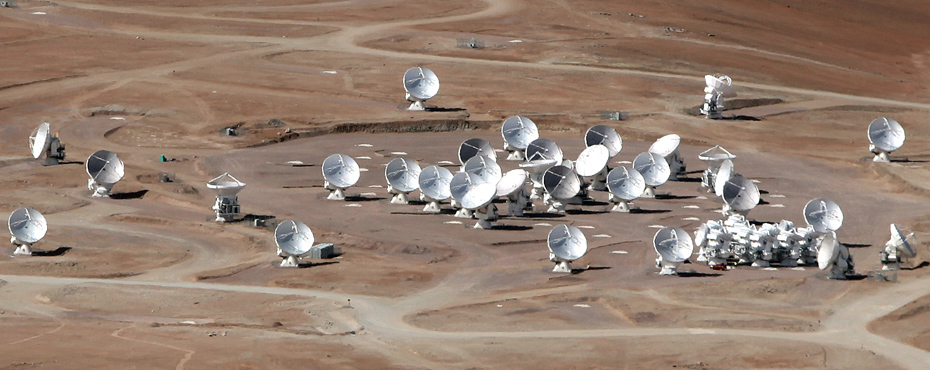
\includegraphics[scale=0.4]{images/Alma.jpg}
	\caption[Observatorio Alma.]{Observatorio Alma. Fuente: \citep{AlmaInt}}
	\label{fig:alma}
\end{figure}

Un interferómetro captura datos por cada par de antenas ($i$ y $j$) (Figura \Ref{fig:antenna}), donde el dato corresponde a la correlación compleja del campo eléctrico que se le denomina visibilidad ($V_{ij}$). Sin embargo, estas corresponden a un muestreo irregular de la transformada de Fourier del mapa de emisión del cielo (plano ($u,v$)). Es decir, esta medición no se realiza en una malla rectangular y existen grandes áreas sin valores medidos \citep{synthesis}. 

\begin{figure}[!ht]
	\centering
	\captionsetup{justification=centering}
	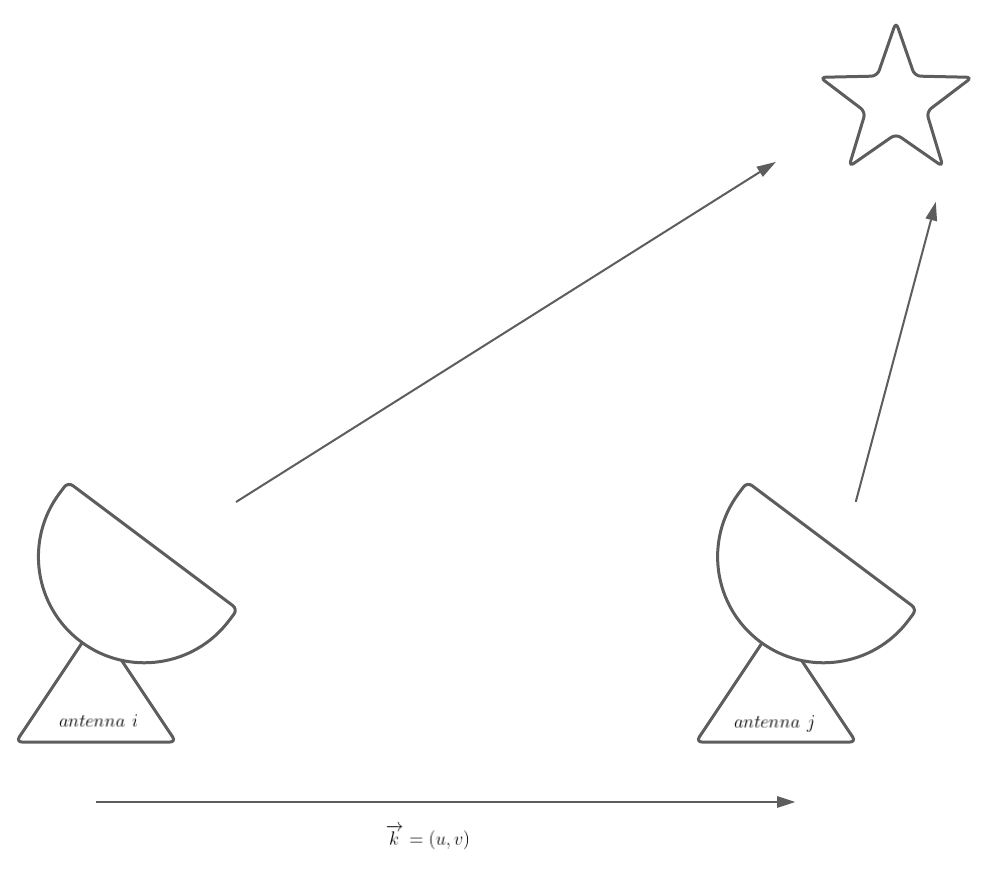
\includegraphics[scale=0.6]{images/antenna_star.png}
	\caption[Captura de datos por interferómetro.]{Captura de datos por interferómetro. Fuente: \citep{carcamo2018multi}}
	\label{fig:antenna}
\end{figure}


La base para lograr la reconstrucción de la imagen es el teorema de Van Cittert Zernike \citep{van1934wahrscheinliche}. Este describe la relación entre la visibilidad $V$ y el mapa de emisión de energía $I$ del cielo (imagen). Las coordenadas $(u,v)$ corresponden a los vectores entre las antenas medidos en metros. Esta relación indica que para obtener una imagen del cielo se debe encontrar la transformada de Fourier inversa. Sin embargo, al no tener los datos regularmente muestreados no es posible utilizar la transformada de Fourier directamente.  

\begin{equation}
    V(u, v) = \int_{-\infty}^{\infty}\int_{-\infty}^{\infty}I(x, y)e^{-2\pi i (ux + vy)}dxdy
    \label{eq:cittert-zernike}
\end{equation}

Adicionalmente, los datos que obtienen las antenas están corruptos por diferentes procesos físicos que inyectan ruido. Las turbulencias en la alta atmósfera agregan un ruido multiplicativo $(g_i)$ (ganancia) a las señales recogidas por cada antena $(i)$. Se asume que varían poco con el tiempo y son solo dependientes de la ubicación de la antena $(i)$. Los receptores de radio de cada par de antenas es afectado por un ruido termal $(\epsilon_{ij})$ Gaussiano y aditivo del instrumento, cuya desviación estándar es $(\sigma_{ij})$ y cambia por cada proceso de muestreo.

%\begin{equation}
 %   \tilde{V}_{ij}(t) = g_{i}(t)g^{*}_{j}(t)V_{ij}(t) + \epsilon_{ij}(t)
 %   \label{eq:error}
%\end{equation}

Existen muchos métodos para reconstruir una imagen a partir de las visibilidades, entre los cuales se pueden encontrar MEM  \citep{wu2012maximum} o CLEAN \citep{clean}. Dichos métodos consideran que $g_i=1$ enfocándose solamente en el ruido aditivo. Aunque existe un método llamado \textit{bispectrum} basado en el producto de tres visibilidades asociadas a tres antenas que conforman un triángulo, se demuestra que dicho producto es invariante ante perturbaciones multiplicativas de fase $(|g_i|=1)$. Esto trae consigo la ventaja de que la imagen generada es menos afectada por el ruido multiplicativo \citep{1958MNRAS.118..276J}.

El error multiplicativo puede ser reducido mediante el método de \textit{self-calibration}. Este tiene como objetivo estimar las ganancias ($g_i$) de las antenas y eliminarlas al dividir las visibilidades observadas por estas ganancias estimadas permitiendo así obtener una mejor calidad de imagen \citep{selfCalibration}. Sin embargo, requiere de un mecanismo de estimación de la imagen. La cual no se encuentra totalmente definida y el astrónomo iterativamente va seleccionando los cambios que mejoran dicha imagen de acuerdo a su conocimiento, experiencia e intuición.

Actualmente con la llegada de instrumentos que generan datos masivos como el producido por el \textit{square kilometer array} (SKA) \citep{ska}, no permitirán que la síntesis de imágenes realizada a través de programación en CPU sea óptima debido a los grandes tiempos de ejecución que se necesita \citep{carcamo2018multi, cottonGPU}. Sin embargo, una opción para incrementar los tiempos de ejecución es la computación paralela que permite realizar diversos procesos al mismo tiempo, trayendo así una ventaja sobre la programación tradicional.

\begin{comment}
Sin embargo, las tarjetas gráficas o GPU son \textit{hardware} que durante los últimos años ya no son solamente utilizadas para juegos, películas 3D e interfaces gráficas, sino que son utilizada para propósitos generales (GPGPU). Esto permite realizar tareas en GPU que tradicionalmente se realizaban en CPU, trayendo consigo la ventaja de acelerar el funcionamiento de aplicaciones de aprendizaje profundo, análisis e ingeniería. Estos dispositivos emplean una arquitectura llamada \textit{Single Instruction Multiple Thread} (SIMT) que permite ejecutar la misma instrucción en el mismo tiempo pero de manera independiente y asíncrona \citep{cheng2014professional}. 
\end{comment}

\section{Descripci\'on del problema}
\label{intro:problema}

Actualmente, la síntesis de imágenes en radio-interferometría se realiza con el framework CASA \citep{bean2022casa}. Dicho framework utiliza la heurística CLEAN tanto para generar imágenes como para calibrar los datos. El investigador en general debe realizar el proceso de calibración de manera manual. Esto tiene la desventaja de demorar el uso final de los datos para la ciencia y que la imagen generada pueda aún tener imperfecciones. Por esta razón los radio-telescopios (e.g. ALMA) disponen de un grupo de expertos con PhD en astrofísica que manualmente experimentan con los datos utilizando CASA para lograr la mejor calibración y poder entregar un producto (datos) de mejor calidad (menos ruidoso) \citep{CasaQA}. 

La nueva generación de radio-observatorios (SKA) espera producir datos a razón de 1 Tb/seg \citep{scaife2020big}. Esto hace prohibitivo el proceso manual de síntesis de imágenes. Esto incluye el proceso previo de de calibración. Es problema es mayor aún ya que dichos datos no podrán almacenarse en ningún dispositivo. Por ello que se van a reducir dichos datos utilizando una técnica llamada gridding \citep{SkaGridding}. Dicha técnica básicamente promedia los datos por celda en una malla regular. Sin embargo, el problema persiste y se requiere que el proceso de calibración sea automático.

Ante esta situación es necesario encontrar métodos y herramientas que permitan calibrar y reconstruir imágenes de buena calidad y de manera autómatica. La calidad de imagen se mide según métricas apropiadas NRMSE \citep{Chael_2018} y PSNR \citep{LiberonaTesis}. Esto enmarcándose en una herramienta que pueda generar resultados dentro de un período corto de tiempo. El método \textit{self-calibration} \citep{selfCalibration} permite eliminar el factor multiplicativo que afecta a los datos. Por otro lado las técnicas de \textit{bispectrum} permite generar algoritmos que no son afectados por el factor multiplicativo. Juntar ambos enfoques puede introducir mejoras a la solución de este problema. Es así que mediante el uso de librerías de cómputo paralelo (e.g Dask \citep{Dask_general}) y las técnicas de self-calibration con {\it bispectrum} se quiere responder a la pregunta de investigación: \textbf{¿Los resultados obtenidos de \textit{bispectrum} dentro de \textit{self-calibration} son mejores, en cuanto a calidad de imagen, que los obtenidos con otros métodos como CLEAN o MEM?}


\section{Soluci\'on propuesta}
\label{intro:solucion}

Este trabajo entrega un estudio para un posible método automático de calibración y síntesis de imágenes en radio-interferometría. Para esto se realiza la creación de módulos para los métodos de \textit{self-calibration} y \textit{bispectrum}, los cuales están dentro del framework Pyralysis \citep{winNT}, el cual está desarrollado en Python y utiliza librerías como Dask, que permite el manejo de grandes conjuntos de datos de manera perezosa, para así aplicar métodos a datos radio-interferométricos. 

Es así que se utilizarán en conjunto el método de \textit{self-calibration} y \textit{bispectrum} para reconstruir imágenes. Donde la síntesis se realiza mediante el método de máxima verosimilitud regularizada, que agrega términos regularizadores y pesos a estos, por lo que se pretende encontrar además los valores óptimos a estos. 

Cabe destacar que el método de \textit{self-calibration} se puede separar en fase y amplitud. Para este trabajo se implementará para ambos casos, donde la fase se debe encontrar los ángulos ($\theta$) que ajusten mejor la visibilidad mediante la formula de ganancias. Por otro lado, la amplitud es encontrar los mejores correcciones de ganancia a las visibilidades. Así como también existe un \textit{bispectrum} para fases y amplitudes, en este trabajo solo se enfoca en el estudio de \textit{bispectrum} en fase. 

En la teoría \citep{selfCalibration} se menciona que para obtener las ganancias asociadas en el método de \textit{Self-calibration} se debe optimizar la ecuación \ref{eq:self-calibration-intro} \citep{selfCalibration}. Sin embargo, en la actualidad las aplicaciones que ha tenido este método se realizan a través de una aproximación que es realizada mediante una divisíon de visibilidades, como es el caso de \citep{gaincal_task} y \citep{rascil}, donde una explicación de el enfoque realizado para este trabajo es detallada más adelante. 
 

%Es así que también es necesaria realizar una comparación entre estos métodos, para así comprender porque no se realiza una optimización de la ecuación \ref{eq:self-calibration-intro}.

\begin{equation}
    \sum |V_{ij} - g_{i}g_{j}^{*}\tilde{V}_{ij}|^2
    \label{eq:self-calibration-intro}
\end{equation}

Los resultados obtenidos serán comparados con los obtenidos mediante los métodos de CLEAN y MEM que son alternativas de solución a la problemática de calibración y reconstrucción de imagen que son utilizadas actualmente. Las métricas utilizadas para comparar es la raíz del error cuadrático medio (NRMSE) que evalúa las imágenes basadas en similitudes píxel a píxel y el \textit{peak signal-to-noise ratio} (PSNR) que compara el valor máximo de la señal y el valor promedio del ruido que la afecta. En la figura \Ref{fig:solucion} se puede ver una representación gráfica de la alternativa de solución propuesta.



\begin{comment}
    Los resultados obtenidos serán comparados con los métodos de CLEAN y MEM. Las métricas utilizadas para comparar es la raíz del error cuadrático medio (NRMSE) que evalúa las imágenes basadas en similitudes píxel a píxel y el \textit{peak signal-to-noise ratio} que compara el valor máximo de la señal y el valor promedio del ruido que la afecta. Así como también, esta última métrica es utilizada para detener el algoritmo de \textit{self-calibration}, ya que al tener un valor mínimo aceptable se detendrá el algoritmo logrando así una automatización del proceso. En la figura \Ref{fig:solucion} se puede ver una representación gráfica de lo propuesto.
\end{comment}

\begin{figure}[!ht]
	\centering
	\captionsetup{justification=centering}
	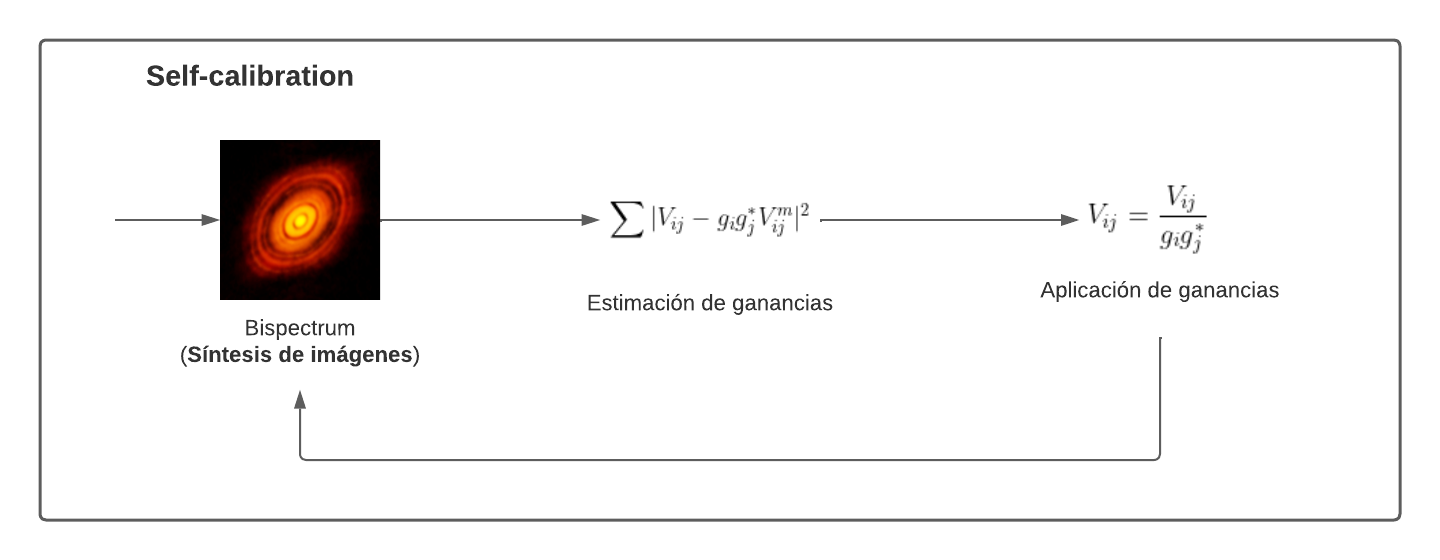
\includegraphics[scale=0.6]{images/solucion.png}
	\caption[Alternativa de solución]{Alternativa de solución. Fuente: Elaboración propia}
	\label{fig:solucion}
\end{figure}

\section{Objetivos y alcance del proyecto}
\label{intro:objetivos}

\subsection{Objetivo general}
Desarrollar una calibración de datos radio-interferometricos basada en \textit{bispectrum} para evaluar si logra una mejor calidad de imagen.

\subsection{Objetivos espec\'ificos}
\begin{enumerate}
    \item Analizar la estructura de los datos y pre-procesamiento de estos. 
	\item Automatizar la reconstrucción de imágenes en base a \textit{bispectrum} a través de un software.
    \item Incorporar el software en el framework de reconstrucción de imágenes Pyralysis.
    \item Implementar el software de reconstrucción de imágenes en base a \textit{bispectrum} usando Dask.
    \item Analizar la aplicación de \textit{Self-calibration} mediante optimización y división. 
    \item Comparar las imágenes obtenidas mediante el método de \textit{bispectrum}, con diferentes pesos de regularizadores, con aquellas reconstruidas con los algoritmos de CLEAN y MEM.
\end{enumerate}

\subsection{Alcances y limitaciones}

La solución adoptada será solamente implementada mediante el lenguaje de programación Python, utilizando el paradigma de orientación a objetos debido a que forma parte del desarrollo para el framework Pyralysis, que permite la aplicación de diversos métodos en conjuntos de datos radio-interferometricos. Además, como los conjuntos de datos a utilizar tanto para este trabajo como en el día a día son de gran tamaño, se debe utilizar la librería Dask que en si es similar a la librería de numpy, ya que contienen las mismas operaciones, pero Dask permite almacenar y trabajar con grandes conjuntos de datos. 

Por otro lado, debido al enfoque del trabajo y considerando los tiempos para este, la implementación realizada solo es se consiodera para los algoritmos de \textit{self-calibration} y \textit{bispectrum}, por lo que los algoritmos de CLEAN y MEM utilizados para comparar no son implementados, sino que se utilizan herramientas existentes como lo son \texttt{tclean} en CASA para el método CLEAN \citep{CASA_clean} y GPUVMEM para el método MEM \citep{carcamo2018multi}. 

Una limitación del software es que este solo podrá ser utilizado para datos que estén en el formato \textit{Measurement Set} (MS) \citep{kemball2000measurementset}. la cual es una base de datos para almacenar datos radio-astronómicos \citep{ms_set}.  

\section{Metodolog\'ia y herramientas utilizadas}
\label{intro:metodologia}

\subsection{Metodolog\'ia}

Para el desarrollo del trabajo toma en cuenta el método científico logrando así generar las siguientes etapas. Cabe destacar que en cada etapa se puede volver hacia alguna anterior de ser necesario. 

\begin{itemize}
    \item \textbf{Investigación}: Corresponde al estudio de los distintos parámetros que afectan los métodos de \textit{self-calibration} y \textit{bispectrum} para así ser implementados, tomando en cuenta así también el trasfondo teórico detrás de estos parámetros. 
    
    \item \textbf{Desarrollo}: En esta etapa se contempla el variar los distintos tipos de parámetros estudiados anteriormente para así obtener la composición que entregue la mejor imagen reconstruida. Para esto se utilizará el \textit{peak signal-to-noise ratio} (PSNR) para saber la calidad de estas.
    
    \item \textbf{Experimentación}: Se realiza la reconstrucción de imágenes a través de \textit{self-calibration} y \textit{bispectrum}, con los parámetros encontrados anteriormente. Además, se realiza la reconstrucción de imágenes mediante \textit{self-calibration} junto a MEM y CLEAN. 
    
    \item  \textbf{Análisis}: Se realiza el estudio y comparación entre las imágenes obtenidas con los distintos métodos mencionados en la etapa de experimentación. Para comparar se utilizará el PSNR o NRMSE de cada una de las imágenes obtenidas mediante los distintos métodos. 
\end{itemize}

Considerando las etapas anteriormente mencionadas, se decide utilizar una metodología ágil, de tal manera de realizar ciclos cortos para entregar avances durante el desarrollo del proyecto. Es así que la metodología utilizada es la denominada metodología en espiral que fue propuesta en \cite{10.1145/12944.12948}, que establece una combinación del enfoque en cascada y el enfoque iterativo. Esta metodología se caracteriza por tener una serie de ciclos de desarrollo que forman una espiral (Figura \ref{fig:spiral_method}), donde cada ciclo consta comúnmente de cuatro fases principales denominadas: Determinación de Objetivos, Análisis del riesgo, Desarrollar y probar y Planificación. De esta manera estas etapas son reemplazadas por las etapas de Investigación, desarrollo, experimentación y análisis mencionadas inicialmente, además que en estas etapas se consideran reuniones con el profesor guía y co-guía para el análisis de avances y problemáticas del desarrollo. 

\begin{figure}[!ht]
	\centering
	\captionsetup{justification=centering}
	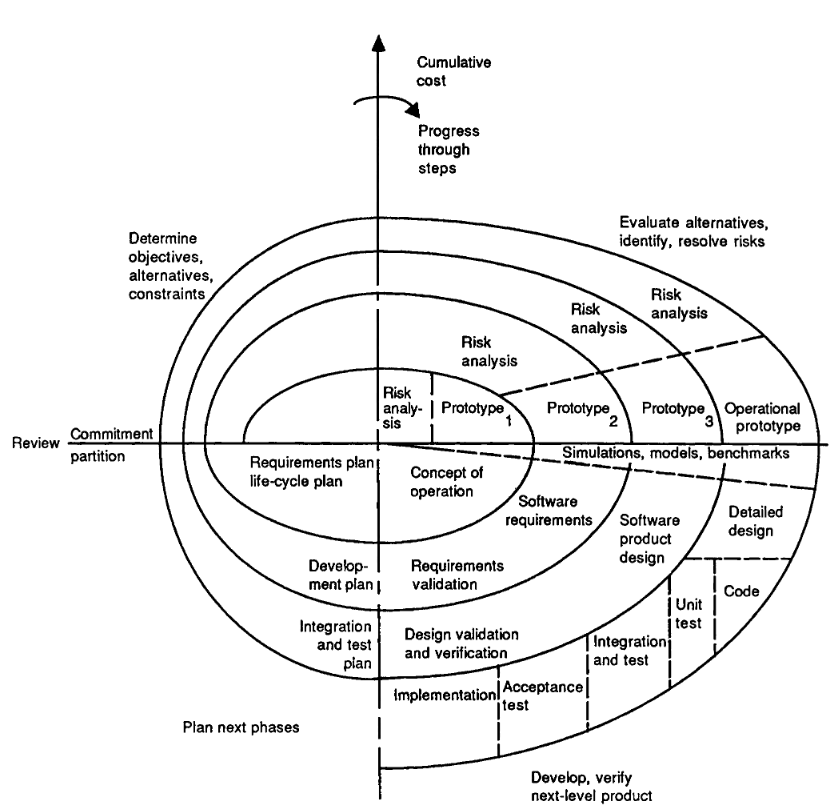
\includegraphics[scale=0.4]{images/Hoen_spiral.png}
	\caption[Metodología en espiral]{Metodología en espiral. Fuente: \citep{10.1145/12944.12948}}
	\label{fig:spiral_method}
\end{figure}

\subsection{Herramientas de desarrollo}

Para el desarrollo de la solución se utilizarán las siguientes herramientas.

\begin{itemize}
    \item \verb|Ubuntu 18.04|: Sistema operativo Linux basado en Debian. 
    \item \verb|Python|: Lenguaje de programación de alto nivel interpretado, que se utilizará junto al paradigma de orientación a objetos (POO).
    \item \verb|numpy|: Librería enfocada en la computación científica de Python.
    \item \verb|dask|: Librería que permite el computo científico de manera paralela en Python.
    \item \verb|numba|: Librería que permite la compilación \textit{Just-in-time}(JIT), que soporta operaciones \texttt{numpy} y \texttt{cupy}.
    %\item \verb|cupy|: Es una libreia de Python que permite la computación acelerada mediante GPU.
    \item \verb|CASA|: Es un software de procesamiento de datos desarrollado por ALMA, que permite el trabajar con datos de antenas radio-interferometricas. 
    \item \verb|GPUVMEM|: Es un framework que permite sintetizar imágenes utilizando una aproximación Bayesiana para resolver el problema.
    \item \texttt{TaQL}: Es un lenguaje de programación similar a SQL que permite realizar operaciones sobre tablas del tipo MS. Su siglas vienen del nombre completo \textit{Table Query Language}.
    \item \texttt{Pyralysis}: Es una librería de Python que combina el uso de este lenguaje con el poder de otras herramientas como Dask para aplicar diferentes métodos a conjuntos de datos radio-interferométricos.  
    \item \texttt{Visual studio code}: Es un editor de código que permite el uso de extensiones que ayudan al desarrollo.
\end{itemize}


Se consideran dos ambientes de trabajo. El primero corresponde al computador personal para el desarrollo del código, donde las especificaciones de este son las siguientes. 

\begin{itemize}
    \item Procesador IntelCore i5-11400.
    \item 32 GB de memoria RAM. 
    \item NVIDIA GeForce GTX 3060ti 8GB
    \item 2 HDD 1TB
    \item 1 SSD 258GB
\end{itemize}

La segunda estación de trabajo considerada es el servidor del departamento de ingeniería informática de la universidad de Santiago de Chile, utilizado para la ejecución de pruebas. Las características de este son las siguientes. 

\begin{itemize}
    \item 2 procesadores Xeon E5-2640.
    \item 256 GB de memoria RAM. 
    \item 4 tarjetas Tesla P100 con SXM2.
    \item 2 HDD 4TB
\end{itemize}


\section{Organizaci\'on del documento}
\label{intro:organizacion}

El documento se organiza de la siguiente manera. En el capítulo 2 se presentan los conceptos básicos para comprender la problemática y solución de este trabajo. Luego en el capítulo 3 se da a conocer el estado actual de implementación que han tenido los métodos de \textit{self-calibration} y \textit{bispectrum}. Siguiente a este, en el capítulo 4, se muestra el análisis necesario para la aplicación de los métodos y siguiente a este, en el capitulo 5 se muestra la implementación realizada según lo visto en el análisis. En el capitulo 6, se muestra los experimentos realizados con las imágenes y métricas asociadas, para luego ser discutidos en el capitulo 7. Finalmente, en el capitulo 8 se mencionan todas las conclusiones sobre el trabajo realizado. 
\chapter{Marco teórico}
\label{cap:marco}

\section{Marco teórico}

El siguiente capítulo describe los fundamentos teóricos necesarios para la comprensión del problema principal planteado en este trabajo, así como también la solución propuesta para este. 

\subsection{Radiointerferometría}

La radiointerferometría se basa en el teorema de Van Citter Zernicke  representado en la ecuación \Ref{eq:cittert-zernike}. Este relaciona directamente la función de visibilidad $V(u,v)$  y el mapa de misión de energia en radio-frecuencias ($I(x,y)$), es decir la imagen que se quiere obtener.  $(x,y)$ representan las coordenadas en radianes de la esfera celeste \citep{synthesis_taylor} y $(u,v)$ es el vector que para una medición use dos antenas en unidades de longitud de onda.

\begin{equation}
    I^{D}(x, y) = \int_{-\infty}^{\infty}\int_{-\infty}^{\infty}V(u, v)S(u,v)e^{-2\pi i (ux + vy)}dudv
    \label{eq:intensity}
\end{equation}

La captura de datos se realiza mediante puntos discretos en la Tierra (antenas) que capturan ondas electromagnéticas denominadas $E_i$. La correlación entre campos eléctricos recibidos por dos antenas ($E_i$ y $E_j$) se le denomina visibilidad y está representada por $V =<E_{i}E_{j}^{*}>$. Si esto se lleva al plano continuo ($u$,$v$) se obtiene lo mostrado en la ecuación \Ref{eq:intensity}.

Un problema es que la  imagen del cuerpo celeste no se puede obtener directamente debido a que el espacio de los datos no se encuentra regularmente muestreado (Figura \Ref{fig:uv_coverage}). Como paso intermedio se traspasan las muestras a una grilla regular lo que generar una gran fracción de celdas sin valor asignado. Esto conlleva a la estimación de $I(x,y)$ llamada imagen sucia, la cual asigna un valor 0 a las celdas sin valor y calcula la trasformada de Fourier. Encontrar una mejor imagen no está bien ya que este es un problema \textit{ill-posed} o mal puesto. Esto significa que desde un mismo conjunto de datos se puede obtener más de una imagen resultante \citep{levanda_art}.


\begin{figure}[!ht]
	\centering
	\captionsetup{justification=centering}
	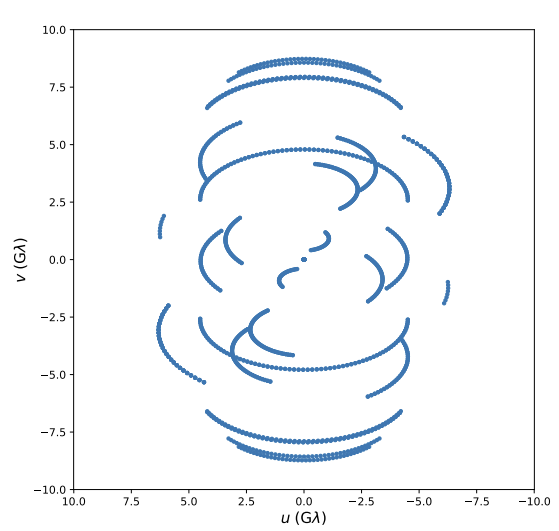
\includegraphics[scale=0.6]{images/uv_coverage.png}
	\caption[Cobertura en el plano $u-v$ para Sagitario A*.]{Cobertura en el plano $u-v$ para observacion de Sagitario A*. Fuente: \citep{Chael_2018}}
	\label{fig:uv_coverage}
\end{figure}

\subsection{Modelo de ruido}

El proceso de captura de datos siempre está sujeto a algún tipo de corrupción. En la radio-interferometría se capturan señales de radio provenientes de lugares lejanos en el espacio exterior, por lo que para llegar al planeta Tierra es necesario que esta señal atraviese distintos medios. Los detectores de señales instalados en cada antena deben ser refrigerados en helio líquido de forma de poder capturar las señales muy débiles \citep{Receivers} y por tanto sujetas al ruido térmico. Es así que los datos radio-interferómetros e imágenes resultantes del proceso de síntesis se encuentran corruptas por factores de ruido. 

Un modelo de ruido \citep{synthesis} utilizado en este trabajo es el presentado en la ecuación \Ref{eq:error2}, que muestra tanto un factor multiplicativo o ganancias y un factor aditivo que afecta a la visibilidad $V_{ij}$ capturada por par de antenas $i$ y $j$. 

\begin{equation}
    \tilde{V}_{ij}(t) = g_{i}(t)g^{*}_{j}(t)V_{ij}(t) + \epsilon_{ij}(t)
    \label{eq:error2}
\end{equation}

El factor multiplicativo o ganancias se produce por las distorsiones atmosféricas al momento de viajar la señal hacia la antena. Por otro lado, el factor aditivo se produce por el ruido térmico en el instrumento. A pesar de ser sometido a temperaturas muy bajas, esto no elimina completamente el ruido. 


\subsection{Síntesis de imágenes}
\label{subcap:sintesis}

La ecuación \Ref{eq:intensity} origina la ecuación \Ref{eq:intensity_conv} cuando se incluye la aproximación a imagen sucia. Donde $b_{0}$ se denomina \textit{beam} sintético y se define como $b_0 = \mathfrak{F}(S(u, v))$, donde $S$ es la función de muestreo. La función de muestreo es simplemente una suma de masas de Dirac ubicadas en las ubicaciones de las mediciones y con intensidad igual al peso.  Examinando la ecuación \Ref{eq:intensity_conv} se entiende que la imagen original se obtendría invirtiendo la operación de convolución . A este proceso se le denomina síntesis de imágenes \citep{synthesis}.  

\begin{equation}
\label{eq:intensity_conv}
    I^{D}(x,y) = I(x,y) **\ b_{0}(x,y)
\end{equation}

Existen diversos métodos para lograr esta deconvolución y así obtener la imagen, como por ejemplo CLEAN \citep{clean} o MEM \citep{sutton2006optimal}. Un método utilizado para la síntesis de imágenes es el utilizado en \citet{Chael_2018}, denominada Máxima verosimilitud regularizada. En esta se realiza la minimización de una función objetivo, donde a esta se le agregan funciones regularizadoras a la falta de información que existe del cuerpo o fenómeno detectado. La ecuación utilizada es la mostrada en \ref{eq:RML}.

\begin{equation}
 \label{eq:RML}
    J(I) = \sum_{data\ terms}\chi_{D}^{2}(I,d) - \sum_{regularizers} \beta_{R}S_{R}(I)
\end{equation}

donde $\chi_{D}^{2}$ es el modulo al cuadrado del residuo en un datos y $S_{R}$ son funciones regularizadoras. Cuyo objetivo es restringir el problema para llegar a una solución única, estas se especifican en \citet{Chael_2018}. Por otro lado, $\beta_{R}$ corresponden a los pesos que se le dan a las funciones regularizadoras correspondientemente. Una imagen reconstruida puede verse en la Figura \Ref{fig:m87}.

\begin{figure}[!ht]
	\centering
	\captionsetup{justification=centering}
	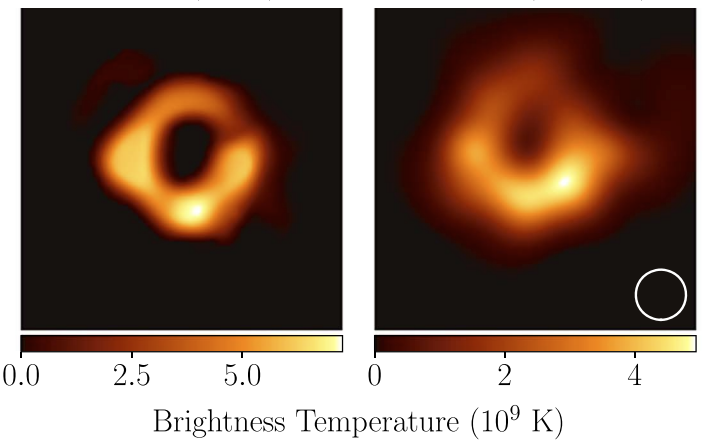
\includegraphics[scale=0.6]{images/Black_hole.png}
	\caption[Imagen reconstruida de agujero negro M87.]{Imagen reconstruida del agujero negro M87 mediante los métodos \textit{Regularized Maximum Likelihood} (RML) (izquierda) y CLEAN (derecha). Fuente: \citep{m87_image}}
	\label{fig:m87}
\end{figure}


\subsection{Datos radio-interferométricos}

Los datos capturados son guardados en un formato llamado \textit{measurement set} (MS) que son un conjunto de carpetas no relacionadas guardadas en disco. A continuación se describe los principales datos utilizados según \citep{kemball2000measurementset}.

\begin{itemize}
    \item \textbf{Visibilidad}: Corresponde al valor de la observación, es decir, el valor resultante de la ecuación \ref{eq:cittert-zernike}. Dicho valor pueden ser guardadas en tres columnas \texttt{DATA}, \texttt{MODEL} o \texttt{CORRECTED}. La columna \texttt{DATA} representa valores medidos en el interferometro o visibilidades observadas. La columna \texttt{CORRECTED} corresponde a valores corregidos por el proceso de {\it selfcalibration}. La columna \texttt{MODEL} son los valores estimados después de la síntesis de imágenes.
    \item \textbf{Pesos}: Es una estimación del valor inverso de la varianza para la visibilidad. Este valor es dado por el correlador. 
    \item \textbf{Antena}: Corresponde a las antenas asociadas a la observación. Estás están separadas en dos columnas denominadas \texttt{ANTENNA1} y \texttt{ANTENNA2}.
    \item \textbf{Tiempo}: Es el instante en el cúal se realizó la medición. 
    \item \textbf{UVW}: Es un vector 3D que une un par de antenas. 
    \item \textbf{Flag}: Indica que si el dato observado esta marcado como invalido, donde Verdadero indica inválido y Falso indica lo contrario. Este tiene las mismas dimensiones que las Visbilidades. 
    \item \textbf{\textit{Scan number}}: Número para identificar aquellas observaciones que se tomaron en el mismo instante. 
\end{itemize}

El software \texttt{casabrowser} \citep{casabrowser} permite acceder a los datos del MS de manera directa. Una tabla vista desde este programa se puede ver en la Figura \ref{fig:casabrowser}. 

\begin{figure}[!ht]
	\centering
	\captionsetup{justification=centering}
	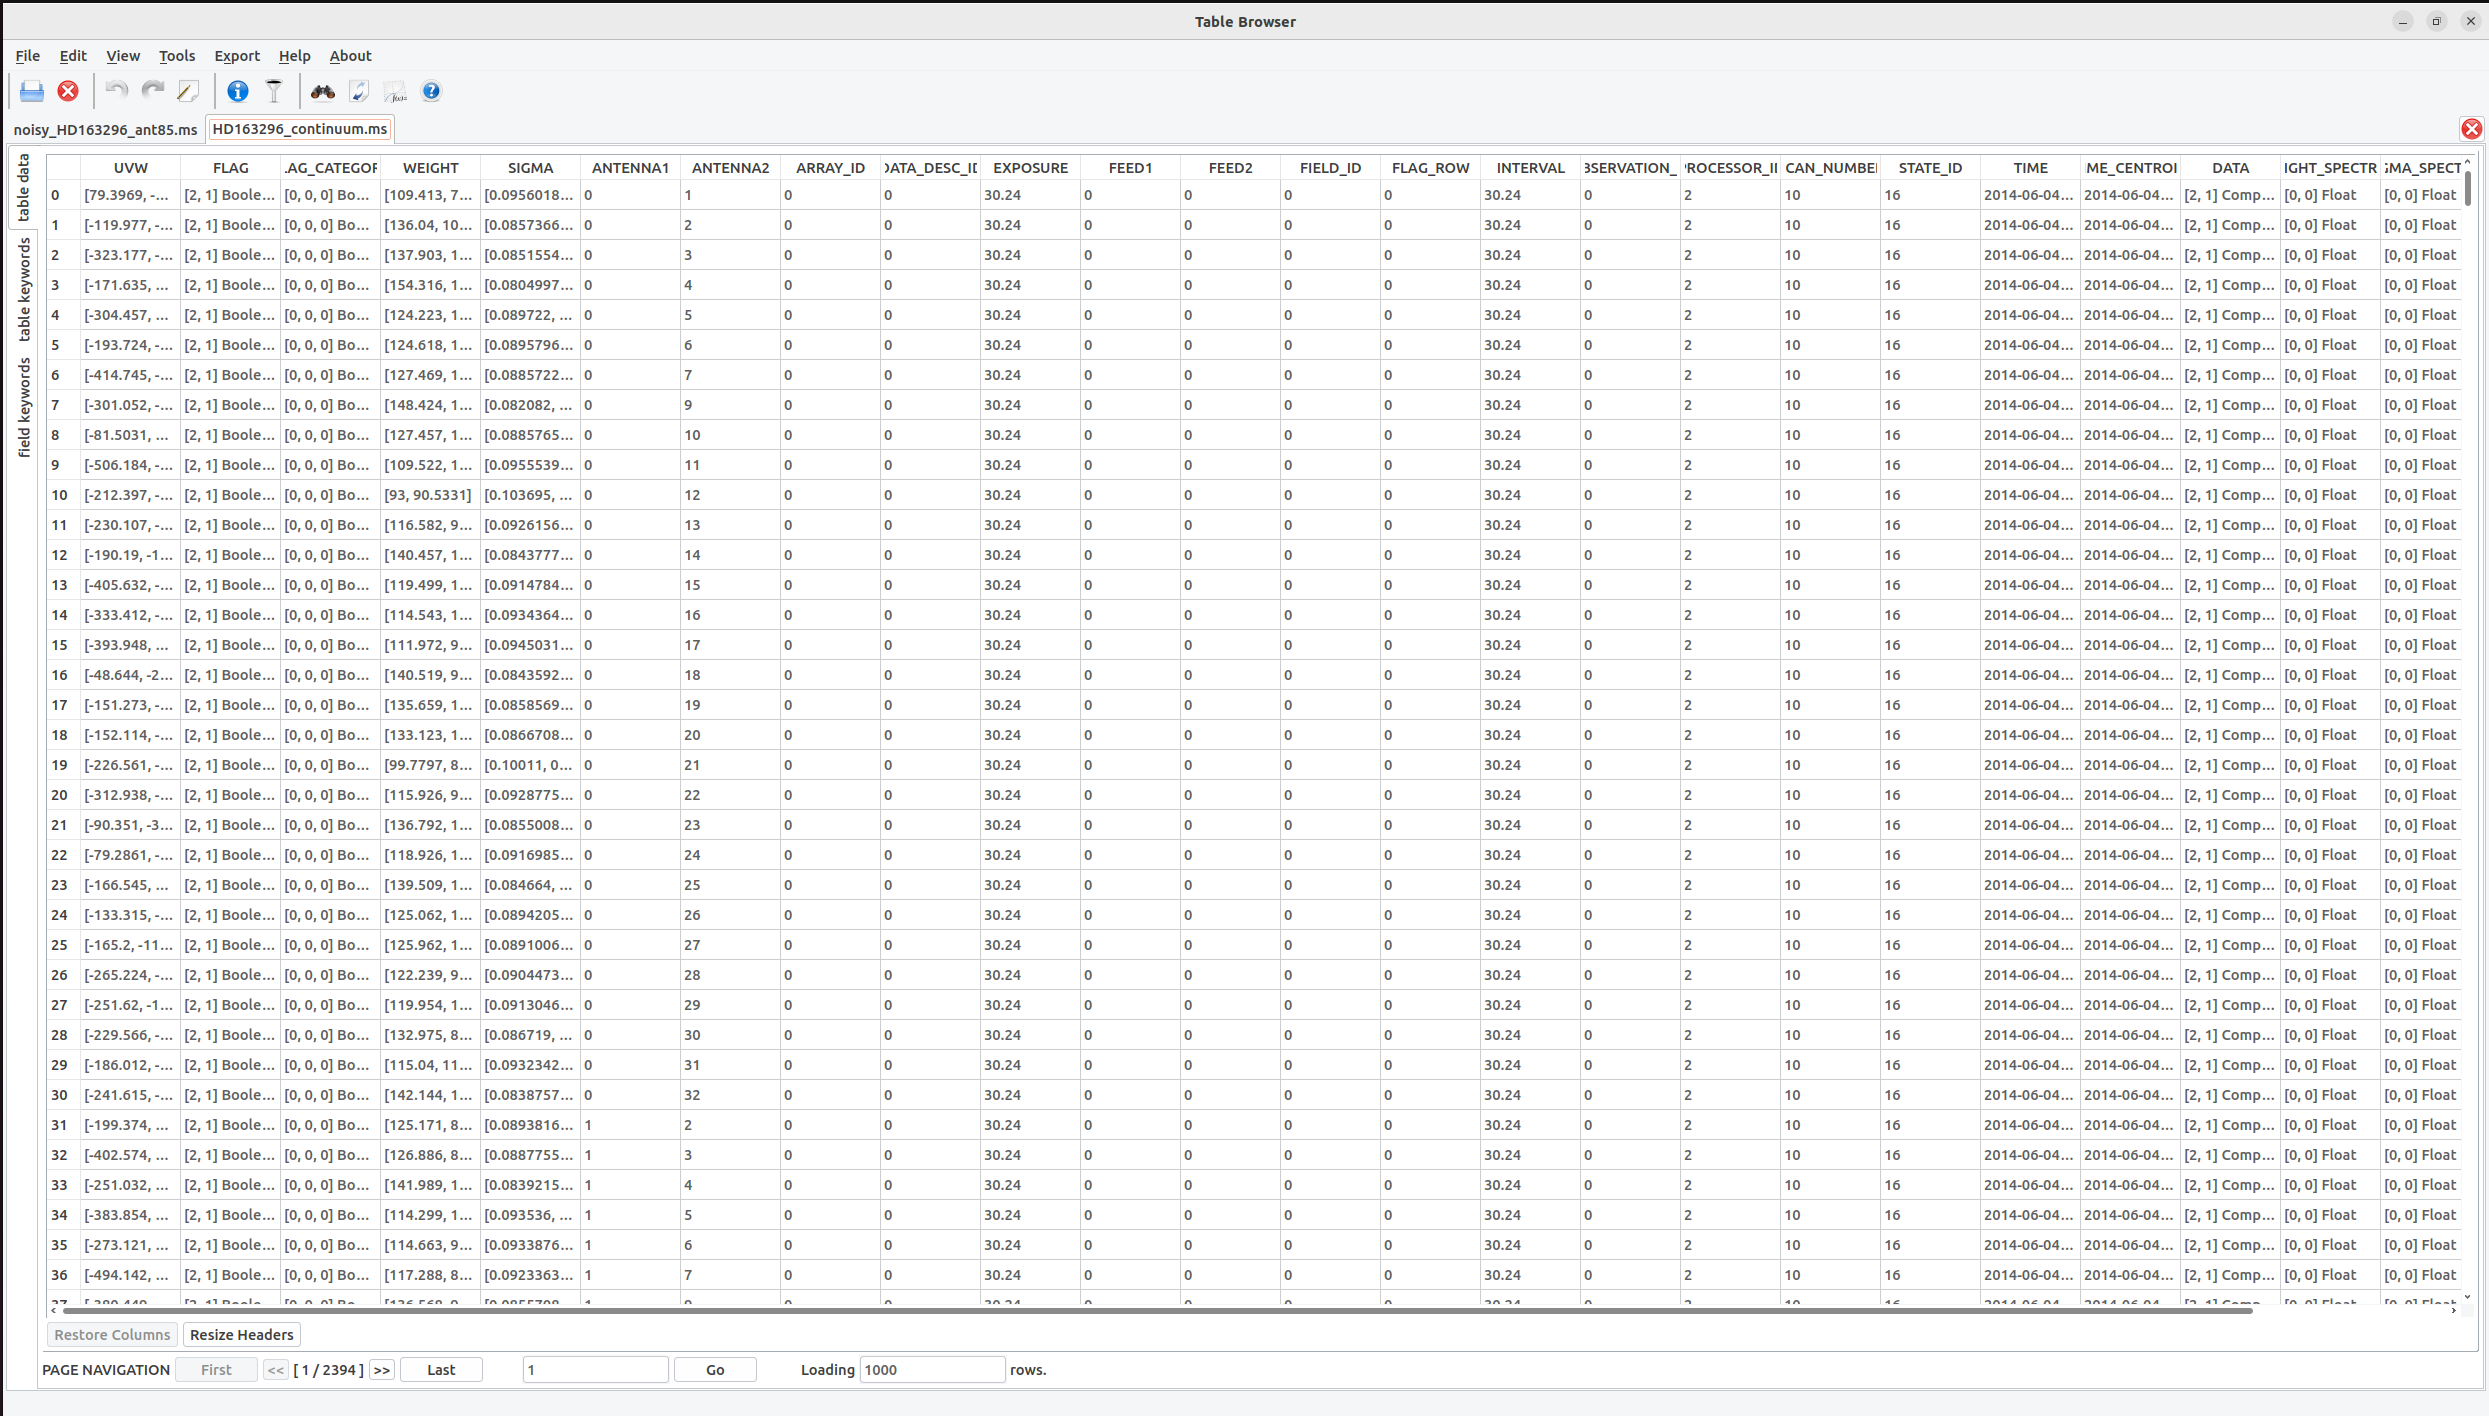
\includegraphics[scale=0.22]{images/casabrowser.png}
	\caption[Casabrowser]{Casabrowser. Fuente: Elaboración propia}
	\label{fig:casabrowser}
\end{figure}



\subsection{\textit{Self-calibration}}
\label{sec:selfcal}

Este procedimiento busca corregir las visibilidades observadas eliminando el ruido multiplicativo generado por turbulencias en la alta atmósfera. Se itera obteniendo un modelo de Imagen $I$ con el cual se obtienen visibilidades modelo con las cuales se estima las ganancias $g_i$ para corregir los datos. Para esto se deben estimar las ganancias $g_i$ y $g_j$ mediante la minimización de la ecuación \Ref{eq:min_self}.
%Este procedimiento busca obtener un modelo de distribución de intensidad $I$, en el cual su transformada de fourier $V$ al ser corregida por unos factores de ganancia se obtiene las visibilidades observadas sin el ruido que le afecta. Para esto se deben estimar las ganancias $g_i$ y $g_j$ mediante la minimización de la ecuación \Ref{eq:min_self}.

\begin{equation}
    S = \sum_{k}\sum_{\genfrac{}{}{0pt}{}{ij\hfill}{i \neq j\hfill}} w_{ij}(t_k) |\tilde{V}_{ij}(t_k) - g_i(t_k)g_{j}^*(t_k)\hat{V}_{ij}(t_k)|^2
    \label{eq:min_self}
\end{equation}

donde $w_{ij}(t_k)$ son pesos, $\tilde{V}_ij(t_k)$ las visibilidades modelo, $\hat{V}_{ij}(t_k)$ las visibilidades observadas y $t_{k}
$ es el intervalo de tiempo donde se obtienen las ganancias. Para corregir estos datos se debe seguir el algoritmo \ref{alg:optSelfCalibration} \citep{selfCalibration}. Cabe destacar que los pasos de este algoritmo se deben repetir hasta encontrar una imagen satisfactoria para el usuario. 

\begin{algorithm}[!ht]
	\caption{Algoritmo de \textit{self-calibration}}
	\label{alg:optSelfCalibration}
	\begin{algorithmic}[1]
	\REQUIRE $I$
	\ENSURE $V_{i,j,corr}$

        \STATE $V_{ij}, \tilde{V}_{ij} \gets reconstruction\_method(I)$

        \STATE $g_{i} , g_{j}^{*} \gets Min( \sum |V_{ij} - g_{i}g_{j}^{*}\tilde{V}_{ij}|^2)$  

        \STATE $V_{i,j,corr} \gets \frac{\tilde{V}_{ij}}{g_{i}g_{j}^{*}}$

        \Return $V_{i,j,corr}$
	
	\end{algorithmic}
\end{algorithm}

\begin{comment}
\begin{enumerate}
    \item Calcular un modelo de datos basado en una imagen modelo ($\tilde{V}=V^{m}(I)$).
    \item Minimizar la ecuación \ref{eq:self-calibration}
    \begin{equation}
        \sum |V_{ij} - g_{i}g_{j}^{*}\tilde{V}_{ij}|^2
        \label{eq:self-calibration}
    \end{equation}
    \item Aplicar los $g_{i}$ encontrados según la ecuación \ref{eq:self-calibration-2}
    \begin{equation}
        V_{i,j,corr} = \frac{\tilde{V}_{ij}}{g_{i}g_{j}^{*}}
        \label{eq:self-calibration-2}
    \end{equation}
    \item Analizar resultado obtenido, en caso de no ser satisfactorio volver a paso 1. 
\end{enumerate}
\end{comment}


\subsection{\textit{Bispectrum}}
\label{subsec:bispectrum}

El interferómetro comúnmente captura datos a través de pares de antenas, denominado visibilidad $V_{ij}$. Sin embargo, si se multiplican los valores de visibilidades de tríos de antenas se consiguen datos que no son afectados en su fase \citep{1958MNRAS.118..276J}. A este dato se le conoce como \textit{closure phase} o \textit{bispectrum} y se le representa mediante $V_{ijk}$ (ecuación \Ref{eq:bispectrum}), siendo $k$ la tercera antena incorporada. De esta manera, en un arreglo de $N$ elementos, se tiene $\frac{1}{2}N(N-1) - (N-1)$ \textit{closure phases}.

\begin{equation}
    V_{ijk} = V_{ij}V_{jk}V_{ki}
    \label{eq:bispectrum}
\end{equation}


Lo anterior puede ser demostrado si se toma la fase de la ecuación \Ref{eq:error3}, se obtiene lo mostrado en la ecuación \Ref{eq:phase}. Una derivación mas detallada de esta ecuación se encuentra en el Anexo \Ref{finales:anexo1}.

\begin{equation}
    \tilde{V}_{ij}(t) = g_{i}(t)g^{*}_{j}(t)V_{ij}(t) + \epsilon_{ij}(t)
    \label{eq:error3}
\end{equation}

\begin{equation}
\label{eq:phase}
    \tilde{\phi}_{ij}(t) = \phi_{ij}(t) + \theta_{i}(t) - \theta_{j}(t) + ruido.
\end{equation}

Donde $\theta_{i}(t) = arg g_{i}(t)$. Si se supone un conjunto de tres antenas $i$, $j$ y $k$, junto con la ecuación \Ref{eq:phase} mostrada anteriormente, se obtiene lo mostrado en la ecuación \Ref{eq:noGain}, donde $\tilde{C}_{ijk}(t)$ es la \textit{closure phase} observado. 

\begin{equation} \label{eq:noGain}
\begin{split}
\tilde{C}_{ijk}(t) & = \tilde{\phi_{ij}(t)} + \tilde{\phi_{jk}(t)} + \tilde{\phi_{ki}(t)}\\
 & = \phi_{ij}(t) + \phi_{jk}(t) + \phi_{ki}(t) + ruido \\
 & = C_{ijk}(t) + ruido
\end{split}
\end{equation}

De la ecuación \Ref{eq:noGain} se desprende que el \textit{bispectrum} no es afectado por el factor de fase en la ecuación de ruido.

El numero total de combinaciones que se pueden dar entre tres antenas esta dada por la ecuación $\binom{N}{3}$ donde $N$ son la cantidad de antenas, esto puede dar una gran cantidad de combinaciones conllevando a una gran carga de trabajo. Para fines de reducir la cantidad de datos se define una antena de referencia para trabajar solo con los tríos de antenas que incluyan a esta antena de referencia. Esto logra que la cantidad posible de combinaciones este dada por la ecuación \ref{eq:comb}, conllevando una disminución en la cantidad de combinaciones y también en la carga de trabajo \citep{Chael_2018}. 

\begin{equation}
\label{eq:comb}
    \binom{N-1}{2} = \frac{(N - 1)(N - 2)}{2}
\end{equation}


\subsection{Métricas de comparación}

\subsubsection{\textit{Peak signal-to-noise ratio(PSNR)}}

Este estimador es utilizado para medir la calidad de la imagen reconstruida, donde se compara el valor máximo de la señal y el valor promedio del ruido que la afecta. Para el contexto de síntesis de imágenes, se entiende como señal a la imagen que se quiere restaurar y al ruido como la diferencia entre la reconstrucción y la imagen original. La fórmula para calcular este estimador está dada por la ecuación \Ref{eq:psnr} \citep{LiberonaTesis}.

\begin{equation}
\label{eq:psnr}
    PSNR = 20 \cdot \log_{10}(\frac{MAX_{I}}{\sqrt{MSE}})
\end{equation}

Si el PSNR aumenta, el resultado se considera mejor pues indica que el brillo del objeto es mayor en comparación al ruido de fondo. Por el contrario, si los valores se parecen, significa que el objeto no se distingue correctamente debido a que se pierde en el ruido de fondo \citep{CeledonTesis}. 


\subsubsection{Raíz del error cuadrático medio (NRMSE)}
\label{sec:nrmse}

El NRMSE por su nombre en inglés \textit{simple normalized root-mean-square error} es una métrica que permite la comparación entre imágenes. Esta es una métrica punto a punto que permite evaluar las imágenes basadas en similitudes píxel a píxel. Por lo que si se tiene una imagen $A$ y una $B$ con $M$ píxeles, el NRMSE de $A$ relativo a $B$ se puede apreciar en la ecuación \Ref{eq:nrmse} \citep{Chael_2018}.

\begin{equation}
    \label{eq:nrmse}
    NRMSE(A,B) = \frac{\sqrt{\sum_{i=1}^{M}(A_i - B_i)^2}}{\sqrt{\sum_{i=1}^M B_{i}^2}}
\end{equation}


\begin{comment}
\subsection{Programación en GPU}

La programación en CPU y GPU tienen su principal diferencia en que la primera tiene un enfoque a ejecutar una secuencia de operaciones (\textit{thread}) lo mas rápido posible y además puede ejecutar una docena de estas en paralelo. En cambio, la tecnología GPU tiene un enfoque para ejecutar cientos de \textit{threads} en paralelo, permitiendo así un tiempo de ejecución menor \citep{nvidiaCuda}. 

Cada función que es llamada desde la CPU (\textit{host}) para ser ejecutada en GPU (\textit{device}) se denomina kernel. Este es ejecutado por $K$ diferentes \textit{CUDA Core}, las cuales son la unidad básica de procesamiento \citep{nvidia_cuda}. Para la ejecución del \textit{kernel}, las hebras son agrupadas en bloques (\textit{blocks}) y estos son agrupados en una grilla (\textit{grid}) que puede tener desde una hasta tres dimensiones \citep{nvidia_programming}. Un ejemplo de grilla y su organización de bloques puede ser vista en la Figura \Ref{fig:grid_nvidia}.

Los bloques son enviados a un \textit{streaming multiprocessor (SM)} para la ejecución del kernel. El multiprocesador crea, maneja, gestiona y ejecuta las hebras en grupos de 32 llamados \textit{warps}. Cada hebra que forma parte del \textit{warp} comienza en la misma dirección del programa, pero cada uno tiene su propio contador de dirección por lo que cada una puede ejecutarse de manera independiente. Además, cada warp tiene su propia memoria compartida \citep{nvidia_hardware}. 

Cuando una grilla junto a sus bloques han sido organizados, se puede identificar una hebra tanto de manera global como local. Para lograr esto existen diversos métodos que se listan a continuación \citep{nvidia_grid}. 

\begin{itemize}
    \item \textit{blockIdx.x, blockIdx.y, blockIdx.z:} identificador del bloque en una grilla para cada una de sus dimensiones. 
    \item \textit{gridDim.x, gridDim.y, gridDim.z:} cantidad de bloques en la dimensión correspondiente de la grilla. 
    \item \textit{threadIDx.x, threadIDx.y, threadIDx.z:} identificador de una hebra dentro de un bloque para cada una de sus dimensiones. 
    \item \textit{blockDim.x, blockDim.y, blockDim.z:} cantidad de hebras en la dimensión correspondiente del bloque. 
    \item \textit{blockDim.x\ blockIdx.x + threadIdx.x:} ID global de la hebra en la dimensión x.  
\end{itemize}

\begin{figure}[!ht]
	\centering
	\captionsetup{justification=centering}
	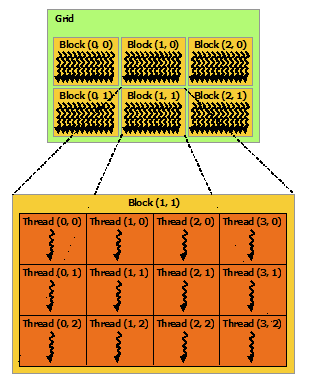
\includegraphics[scale=0.6]{images/grid_nvidia.png}
	\caption[Organización de grilla GPU.]{Organización de grilla GPU. Fuente: \citep{nvidia_programming}}
	\label{fig:grid_nvidia}
\end{figure}
\end{comment}

\subsection{Programación orientada a objetos (POO)}

La idea principal de la programación orientada a objetos (POO) es programar en términos de objetos y clases de tal manera de representar la vida real (Figura \Ref{fig:poo_image}). Este ultimo se entiende como un modelo o plano para poder crear objetos, permitiendo así guardar datos y funcionalidades. En cambio, los objetos son instancias de una clase, las cuales tienen métodos y atributos que intentan simular un objeto de la vida real. Algunos conceptos a tener en consideración son los siguientes \citep{tatachar2021object}. 

\begin{itemize}
    \item \textbf{Atributos:} Valores que son contenidos dentro de la clase. Estos pueden ser atributos de clases que son aquellos que se comparten entre todos los objetos, o pueden ser atributos de instancia, que son aquellos asociados a un objeto. 
    \item \textbf{Métodos:} Son funciones asociadas al objeto que permiten el comportamiento de este.
    \item \textbf{Herencia:} Característica que permite a una clase heredar los atributos y métodos de una clase padre o superior. 
    \item \textbf{Polimorfismo:} Permite que una acción sea ejecutada de distintas maneras. Por ejemplo, la operación suma en Python tiene diferentes resultados cuando se realiza con enteros o con \textit{strings}.
\end{itemize}

\begin{figure}[!ht]
	\centering
	\captionsetup{justification=centering}
	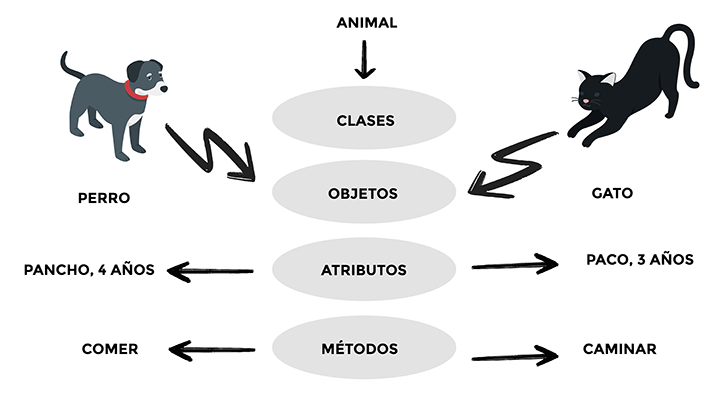
\includegraphics[scale=0.6]{images/POO.png}
	\caption[Ejemplo de abstracción del mundo real a POO.]{Ejemplo de abstracción del mundo real a POO. Fuente: \citep{poo_image}}
	\label{fig:poo_image}
\end{figure}

\subsection{Patrones de diseño}
\label{subsec:patrones}

Una definición bien utilizada para estos puede ser encontrada en  \cite{gamma2002patrones}, donde se menciona que los patrones de diseños son descripciones de objetos y clases interconectados que se adaptan para solucionar problemas de diseño generales en contextos específicos. Para esto un patrón de diseño debe contar con lo siguiente: 

\begin{itemize}
    \item \textbf{Nombre de patrón}: Sirve para describir el problema, la solución y la consecuencia en una o dos palabras. De esta manera se amplia el vocabulario de los patrones, permitiendo una mejor comprensión y comunicación de este. 
    \item \textbf{Problema}: Cuando aplicar el patrón de diseño. Este puede ser tanto de problemas de diseño específicos o describir estructuras de clases u objetos que son sintomáticas de un diseño inflexible. Además estos pueden incluir condiciones que especifiquen si se puede ocupar o no el patrón de diseño. 
    \item \textbf{Solución}: Son los elementos que contribuyen al diseño, sus relaciones, responsabilidades y colaboraciones. Es una plantilla abstracta que se adapta a diferentes situaciones, ofreciendo una solución general a un problema de diseño. 
    \item \textbf{Consecuencia}: Este es el resultado y compensación de aplicar el patrón de diseño, y son fundamentales para realizar un análisis para así comprender los costos y beneficios de su implementación. Entre las consecuencias que puede traer un patrón de diseño se considera su impacto en la flexibilidad, extensibilidad o portabilidad de un sistema.
\end{itemize}

Entre los patrones de diseño existentes en la realidad se puede encontrar el \textit{Decorator}, que permite añadir nuevas funcionalidades a un objeto dinámicamente a través de encapsular el objeto con otro objeto. Un diagrama de objetos que representa esta implementación es el mostrado en la figura \ref{fig:gamma2002patrones} y una implementación sencilla de código Python puede ser encontrada en el apéndice \ref{finales:apendice2}.

\begin{figure}[!ht]
	\centering
	\captionsetup{justification=centering}
	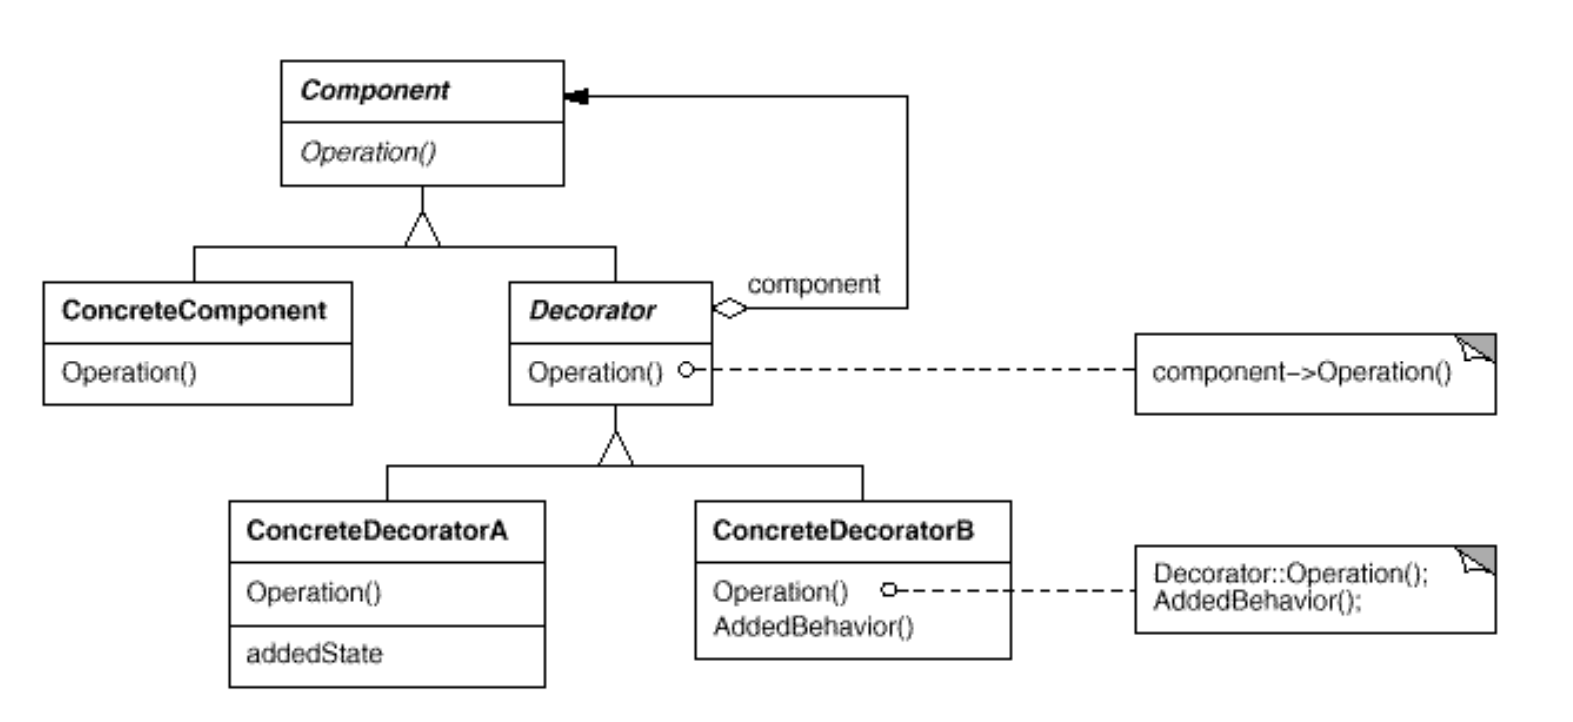
\includegraphics[scale=0.3]{images/decorator.png}
	\caption[Patrón de diseño Decorator.]{Patrón de diseño Decorator. Fuente: \citep{gamma2002patrones}}
	\label{fig:gamma2002patrones}
\end{figure}

Entre las ventajas que se encuentran del patrón de diseño \textit{Decorator} son no influir en las funcionalidades de otros objetos de la misma clase, así como también permite ejecutar funcionalidades del componente mismo, por lo que se pueden realizar acciones antes o después de esta ejecución. Además permite evitar la creación de clases cargadas de funcionalidades en lo alto de la jerarquía debido a que se puede crear una clase simple y agregar funcionalidades de manera incremental a través de decoradores. 

Sin embargo, las desventajas de este son que el componente y el decorador no son iguales desde el punto de vista de la identidad del objeto, debido a que el decorador solamente es un envoltorio. Por otro lado, aumentan la complejidad del código ya que existen muchos objetos pequeños que se parecen pero la manera en la que están interconectados difieren. 


\subsection{Pyralysis}
\label{subsec:pyralysis}

\textit{Python Radio Astronomy Analysis and Image Synthesis} (\textit{Pyralysis}) es un framework desarrollado en el lenguaje de programación Python junto a el paradigma de orientación a objetos (POO). Este tiene como objetivo facilitar el trabajo de los investigadores al tratar con datos radio-interferometricos automatizando procesos. Este framework actualmente se encuentra en desarrollo, pero mayor información puede ser encontrada en su repositorio de Gitlab \citep{winNT}.

\subsection{Computación paralela}

La computación paralela permite ejecutar varias instrucciones al mismo tiempo \citep{parallel}, por lo que para aprovechar esto en la programación existen diversas herramientas como es el caso de Dask, la cual es una librería para computo paralelo en Python \citep{Dask_general}. Dentro de Dask existe una colección conocida como \verb|Dask.array|, la cual es una copia de la interfaz de Numpy y permite separar grandes arreglos de datos en unos mas pequeños denominados bloques y que se ordenan a través de una grilla \citep{Dask_array}.  

\begin{figure}[!ht]
	\centering
	\captionsetup{justification=centering}
	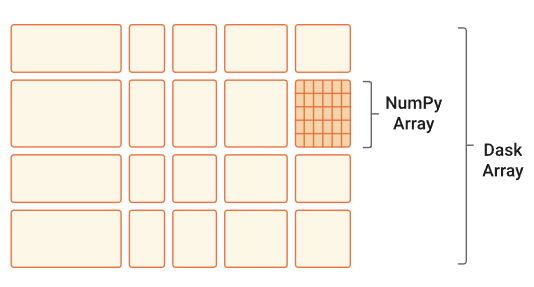
\includegraphics[scale=0.6]{images/dask_array.png}
	\caption[Organización de Dask array.]{Organización de Dask array. Fuente: \citep{Dask_array}}
	\label{fig:dask_array}
\end{figure}

Estos grandes arreglos son divididos en \textit{chunks} para así lograr el procesamiento paralelo y distribuido, por lo que se debe escoger un buen valor para estos ya que puede afectar de manera negativa el rendimiento en caso de una mala elección \citep{Dask_chunks}. Los \textit{chunks} tiene un tamaño firme y uniforme, el cual debe ser de un tamaño lo suficientemente pequeño para caber en memoria pero lo suficientemente grandes para que las tareas se ejecuten hasta en 1ms, normalmente estos van desde 10MB hasta 1GB. 

\begin{figure}
 \centering
  \subfloat[Arreglo Original]{
   \label{fig:chunk_or}
    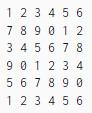
\includegraphics[width=0.2\textwidth]{images/chunk_or.png}}
  \subfloat[Arreglo con \textit{chunks} igual a 3]{
   \label{fig:chunk_3}
    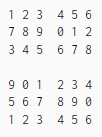
\includegraphics[width=0.19\textwidth]{images/chunk_3.png}}
    \subfloat[Arreglo con \textit{chunks} igual a (3,2)]{
   \label{fig:chunk_32}
    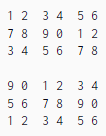
\includegraphics[width=0.2\textwidth]{images/chunk_32.png}}
 \caption[Arreglo dividido por chunks]{Arreglo dividido por \textit{chunks}. Fuente: \citep{Dask_chunks}.}
 \label{fig:chunks}
\end{figure}


Para lograr una computación paralela \verb|Dask.array| trabaja con grafos, es decir transforma las tareas de Python en un formato que implica tuplas, diccionarios y funciones. Es así que un grafo de dask se define como un diccionario que mapea hacia llaves y valores. Donde una tarea es una tupla en el cual su primer elemento es invocable y una llave es cualquier cosa que no sea una tarea \citep{rocklin2015dask}.

\begin{figure}[!ht]
	\centering
	\captionsetup{justification=centering}
	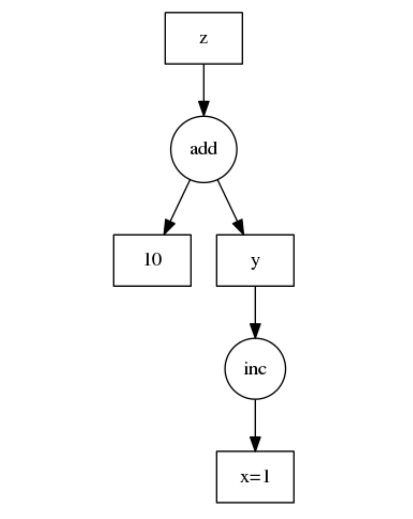
\includegraphics[scale=0.6]{images/grafo_dask.png}
	\caption[Ejemplo de grafo en dask.]{Ejemplo de grafo en dask. Fuente: \citep{rocklin2015dask}}
	\label{fig:dask_graph}
\end{figure}

\verb|Dask.array| es capaz de soportar la mayoría de las funcionalidades de Numpy como por ejemplo la operaciones aritméticas (+, - , *, exp, log, etc.), particionamiento, reducciones en los ejes (sum(), mean(), std()), álgebra lineal, indexación, entre otros. Sin embargo, no soporta algunas operaciones para arreglos con alguna dimensión con valor nulo, la mayoría de \verb|np.linalg| no está implementado, no implementa operaciones como \verb|tolist|, entre otros.

\newpage

\chapter{Estado del arte}
\label{cap:estado}

\section{Bispectrum}

En \citet{Chael_2018} se aplicó un método de reconstrucción de imágenes utilizando el método de Máxima verosimilitud regularizada con datos \textit{closure only} (o \textit{bispectrum}. Se utiliza una antena de referencia con el objetivo de poder reducir la cantidad de posibles combinaciones y así también lograr un mejor rendimiento del software. Además se realiza una comparación con imágenes reconstruidas mediante \textit{bispectrum} y \textit{self-calibration} tanto para datos simulados como para datos de VLBA y ALMA. Sin embargo, lo realizado en \citet{Chael_2018} no está enfocado en \textit{self-calibration}. Se especifica que los pesos de los regularizadores sea óptimo y por otro lado, el método de optimización utilizado no es el mejor ya que asume diferenciabilidad. Se presentan mejores resultados que lo obtenido con el método \textit{self-calibration} junto a CLEAN, pero queda la interrogante de si \textit{self-calibration} junto a \textit{bispectrum} es una buena alternativa. Esta tesis se enfoca en este último aspecto.

Siguiendo al mismo autor, en \citet{event_horizon} se explora una variante del algoritmo MEM para observaciones obtenidas mediante \textit{Very Long Baseline Interferometry} (VLBI). Esta variante se le denomina algoritmo MEM polarimétrico, donde se combina un generador de imágenes polarizadas Stokes I que solo utiliza mediciones de bispectrum junto a generadores de imágenes Stokes Q y U que operan con relaciones polarimétricas robustas. De esto se obtienen resultados con mejor resolución que los obtenidos con CLEAN, cuando se trata de imágenes de distribuciones de fuentes suaves y compactas. 

En \citet{m87} se estudia la variabilidad de las imágenes reconstruidas para el agujero negro ubicado en el centro de la galaxia M87. Para esto se utilizan datos del tipo \textit{closure phases} o \textit{bispectrum}, de tal manera de analizar la variabilidad que tienen estos datos. De esto se obtuvo que los únicos triángulos que presentaban una gran variabilidad ($\sim$90 - 180$^o$) son aquellos cuyas baselines cruzan la amplitud de visibilidad mínima en el plano $uv$. Aún así se encuentra que tres triángulos presentan poca variabilidad ($\sim$3 - 5$^o$). 

\textit{Bispectrum} también a sido estudiado en \citet{geometry}. En este se muestra el principio de conservación forma-orientación-tamaño o SOS por su traducción al ingles, donde se dice que, la cualidad de que las \textit{closure-phases} no esten afectadas por el ruido multiplicativo esta relacionada a la forma y orientación del triangulo entre las tres antenas. El principio de conservación SOS permite la aplicación de dos métodos para obtener los datos \textit{closure phases} directamente desde el plano de la imagen. El primero permite estimarlo geométricamente en el plano de la imagen a partir de una única medición de cualquiera de las alturas del triangulo delimitado por las tres franjas principales. El segundo permite la estimación a partir de una relación invariante que existe entre la \textit{closure phase} al cuadrado y el productor de las áreas encerradas por la triada de elementos en el plano de apertura y el triangulo encerrado por las tres franjas en el plano de la imagen. 

Una nueva técnica para síntesis de imágenes es propuesta en \citet{akiyama2017imaging} donde se propone utilizar la amplitud de las visibilidades y el \textit{closure phase} a través de las funciones de regularización $\ell_{1}$-norm y la variación total (TV) de la distribución del brillo, así como también la técnica \textit{cross-validation} (CV) para obtener los mejores valores para los parámetros $\eta_{l}$ y $\eta_{t}$. Para la realización de esto se minimiza la ecuación \ref{eq:paper_min}. 

\begin{equation}
    \label{eq:paper_min}
    C(I) = \chi^{2}(I) + \eta_{l} ||I||_{1} + \eta_{t} ||I||_{tv}
\end{equation}

El primer término de esta representa la desviación entre la imagen reconstruida y las visibilidades observadas. Este término esta dado por la ecuación \ref{eq:aki_eq1} donde $A(FI)$ y $B(FI)$ representan los operadores para calcular las amplitudes y las \textit{closure phases}. El segundo término representa la regularización tipo LASSO usando $\ell_{1}$-norm y el tercer término representa la regularización TV definida por la ecuación \ref{eq:aki_eq2}.

\begin{equation}
    \label{eq:aki_eq1}
    \chi^{2}(I) = || \bar{V} - A(FI)||^{2}_{2} + || \Psi - B(FI) ||^{2}_{2}
\end{equation}

\begin{equation}
    \label{eq:aki_eq2}
    ||I||_{tv} = \sum_{i} \sum_{j} \sqrt{|I_{i+1j} - I_{ij}|^{2} + |I_{ij+1} - I_{ij}|^{2}}
\end{equation}

Finalmente, los resultados obtenidos indican que se puede alcanzar una resolución óptima de $\sim20\% - \sim30\%$ del límite de difracción $\lambda / D_{max}$ que es la resolución espacial nominal del radio-interferometro. Sin embargo, una acotación hecha es que este método se podría mejorar utilizando \textit{self-calibration} debido a la perdida de información que se sufre a utilizar técnicas como \textit{closure-phases}. 

\textit{Bispectrum} es utilizado en \citet{bowersobservations} para reconstruir imágenes de sistemas de estrellas binarias, esto para así aprovechar eliminar el ruido atmosférico que puedan tener las imágenes. El objetivo de este articulo es determinar si las estrellas observadas son estrellas dobles físicas o par binario, que son aquellas estrellas conformadas por una mas brillante que la otra y orbitan alrededor de un baricentro. Para esto se utilizaron los datos de \textit{Boyce Astro Robotic Observatory} que consisten entre 500 a 1000 imágenes con una exposición entre 0.01 a 1 segundos. Las imágenes obtenidas se pueden observar en la Figura \ref{fig:bin_star}. Los resultados indican que las observaciones 3 y 7 están atados gravitacionalmente mientras que 1 y 2 no lo están, por otro lado, las observaciones 4, 6 y 8 son binarios pero con la observación 5 se mantiene en duda debido a que el resultado obtenido difiere significativamente con los datos históricos de esta observación. 

\begin{figure}[!ht]
	\centering
	\captionsetup{justification=centering}
	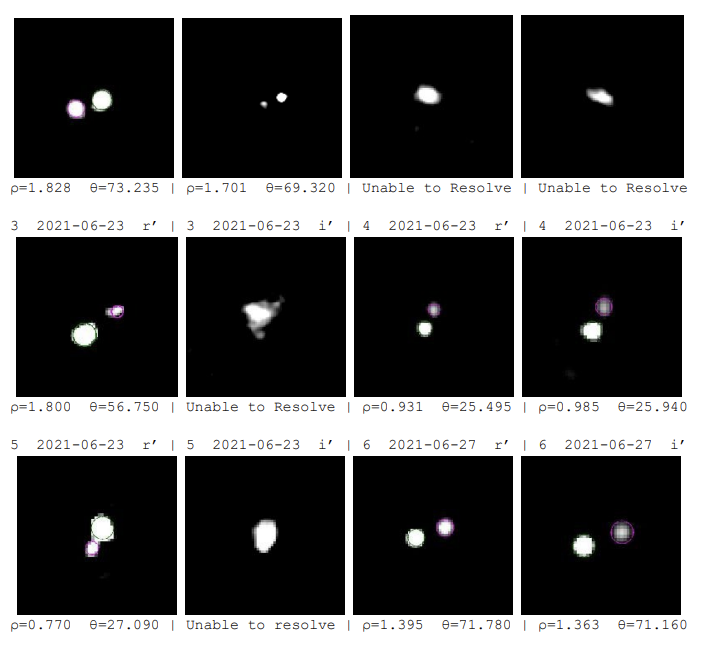
\includegraphics[scale=0.6]{images/pares_estrellas.png}
	\caption[Sistema de estrellas binarias]{Imágenes obtenidas mediante el método de Bispectrum para sistema de estrellas binarias. Cada subfigura contiene la estrella más brillante (círculo verde) y la menos brillante (círculo morado), así como también la separación ($\rho$) y ángulo ($\theta$) para cada observación. Fuente: \citep{bowersobservations}}
	\label{fig:bin_star}
\end{figure}

\section{Self-calibration}

El método de \textit{self-calibration} es utilizado en \citet{cook_seymour_sokolowski_2021} para la calibración de datos obtenidos por el proyecto \textit{Murchinson Widefield Array} (MWA). En altas frecuencias aparecen \textit{sidelobes}, que dificultan el procesamiento de la imagen y la calibración, donde para MWA esto ocurre a los $\sim$ 350 MHz. Sin embargo, en este trabajo se propone un nuevo método de calibración donde se crea un modelo del cielo que ha sido interpolado en altas y bajas frecuencias, el cual es sometido a un ciclo de \textit{self-calibration} que es utilizado para crear una mascara de las visibilidades. Esto abre las posibilidades de poder trabajar a frecuencias de 300 MHz para MWA. 

En \citet{ortiz} se estudia la forma intrínseca del agujero negro supermasivo Sagitario A*, que se encuentra en el centro de la Vía Láctea. En este se realiza una comparación entre lo obtenido con solamente \textit{closure amplitudes} y lo obtenido con \textit{self-calibration}. De los análisis realizados se da a conocer que ambos enfoques son adecuados para obtener resultados consistentes 

\begin{comment}
    Una implementación en GPU puede ser encontrada en \citet{GPU}, donde realiza una implementación de un algoritmo \textit{bispectrum} con usos de GPU. En este se realiza una comparación para la obtención de \textit{radio transients}, que son estallidos de radiación electromagnética, de una implementación multi-thread en CPU y una implementación GPU con CUDA. Esto da como resultado que el algoritmo \textit{bispectrum} es eficiente tanto en CPU como GPU, donde el primero obtuvo un \textit{speed-up} de 3.2x y el segundo obtuvo un \textit{speed-up} 20 veces mas que el primero. 
\end{comment}

\textit{Common Astronomy Software Applications} (CASA) \citep{bean2022casa} es el principal software utilizado para los observatorios ALMA y VLA, aunque también utilizado en otros observatorios. Este software es capaz de manejar datos telescópicos, donde su principal objetivo es la calibración de estos y la reconstrucción de imágenes con estos. De esta manera, en CASA se puede encontrar una implementación para el método de \textit{self-calibration}, sin embargo no es posible encontrar una implementación para el método de \textit{Bispectrum}. Aunque el primer método es mayormente utilizado mediante este software, este tiene que ser ejecutado por el experto de manera manual, es decir, ejecutar comando por comando todo el algoritmo presentado en la sección \Ref{sec:selfcal}. Un script de ejemplo para esto puede ser encontrado en el Anexo \ref{finales:anexo2}, así como también una imagen resultante de todo el proceso se puede ver en la Figura \ref{fig:selcal_comp}.

\begin{figure}
 \centering
  \subfloat[Imagen residual original]{
   \label{fig:original}
    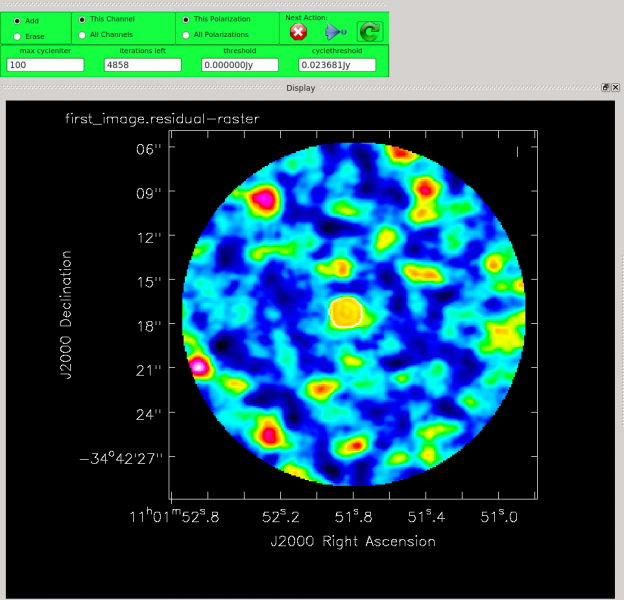
\includegraphics[width=0.4\textwidth]{images/original_casa.png}}
  \subfloat[Imagen residual luego de cuatro ciclos]{
   \label{fig:four}
    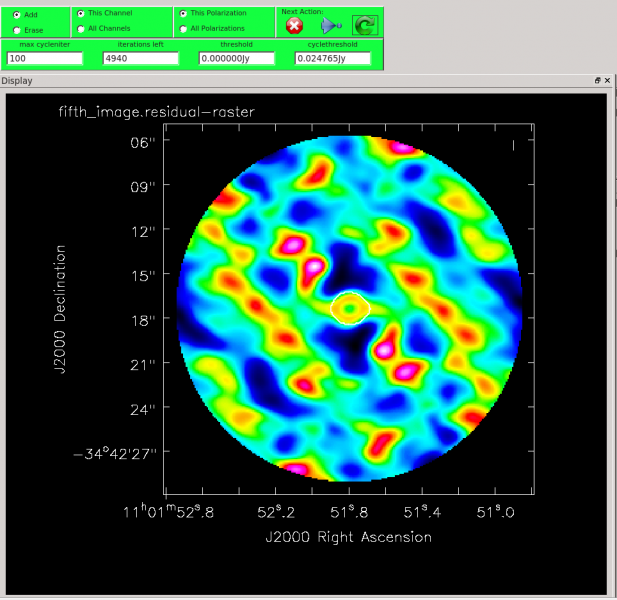
\includegraphics[width=0.4\textwidth]{images/four_self_casa.png}}
 \caption[Imagenes residuales CASA self-calibration]{Imágenes residuales de conjunto de datos TWHydra. Fuente: \citep{CASA_self_cal}.}
 \label{fig:selcal_comp}
\end{figure}

En \cite{FernandezTesis} se presenta una implementación de \textit{self-calibration} utilizando redes neuronales profundas a través de \textit{Amazon Web Services (AWS)}. Se entrena una red con imágenes perturbadas con un error conocido, donde se es capaz de predecir el error que tenga el conjunto de datos. Las redes entrenadas son iguales a las cantidades de antenas y se selecciona la predicción que presente la mayor mejora en la imagen mediante la comparación del valor del PSNR. De esto se obtiene un método automatizado y factible que es capaz de obtener mejoras en imágenes utilizando \textit{self-calibration}. Un resultado obtenido se puede observar en la Figura \ref{fig:tesis_fer}.

\begin{figure}[!ht]
	\centering
	\captionsetup{justification=centering}
	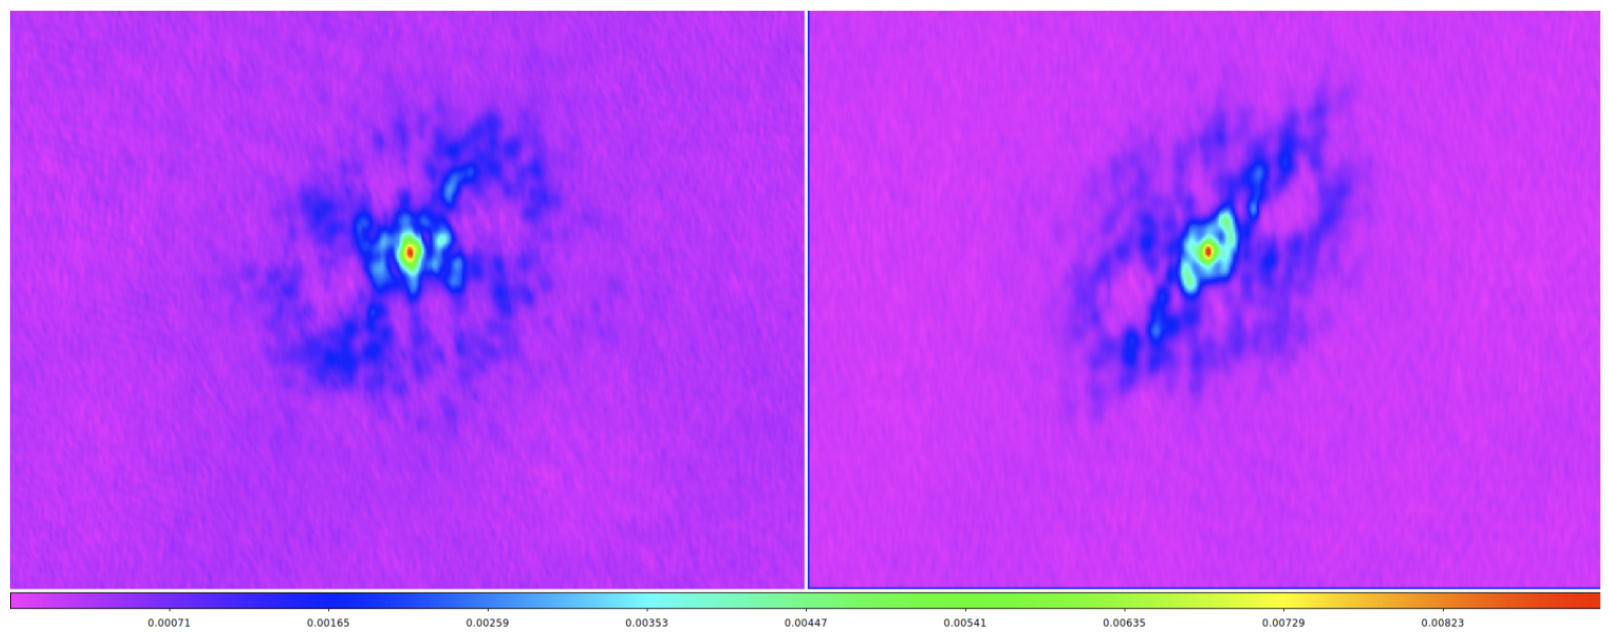
\includegraphics[scale=0.3]{images/self_cal_tesis.png}
	\caption[Resultado de Selfcal con redes neuronales]{HL-TAURI con ruido (izquierda) y con Selfcal (derecha). Fuente: \citep{FernandezTesis}}
	\label{fig:tesis_fer}
\end{figure}

\chapter{Análisis}
\label{cap:analisis}

En este capitulo se detalla los diferentes análisis realizados para poder implementar los métodos de \textit{self-calibration} y \textit{Bispectrum}, de tal manera de obtener una buen resultado de estos métodos. 

\section{Pyralysis}

Un aspecto importante para el desarrollo de los métodos \textit{Bispectrum} y \textit{Self-calibration} es el formato de los datos a trabajar. Los conjuntos de datos utilizados vienen en formato \textit{measurement set} (MS) que permite el almacenamiento de visibilidades en tablas \citep{kemball2000measurementset},  el cual extiende el formato AIPS++ definido por \cite{cornwell1997design} que almacenaba los datos generados a través de clases en el lenguaje C++. No obstante, el formato a trabajar es el entregado por el framework Pyralysis, el cual lee el conjunto de datos en su formato MS y lo transforma a un objeto de Pyralysis. Este permite un fácil acceso a información relevante, como las visibilidades observadas y modelo, las antenas asociadas a estas, el tiempo de medición, los pesos, entre otros datos. De esta manera, se debe tener en consideración el formato de Pyralysis ya que los métodos de \textit{Bispectrum} y \textit{self-calibration} se deben implementar dentro de este framework.

Como se menciona en la sección \ref{subsec:pyralysis}, Pyralysis es un framework que utiliza la programación orientada a objetos, por lo que los datos y funcionalidades de este son accesibles a través de clases que contienen atributos y métodos. Estas clases son importantes a considerar para la implementación de los métodos de \textit{self-calibration} y \textit{Bispectrum} debido a que se utilizarán en conjunto con las nuevas clases necesarias para la implementación de los métodos antes mencionados. 

\begin{itemize}
    \item \textbf{DaskMS}: Clase de I/O que permite el manejo de los conjuntos de datos en su formato MS, además de su escritura y lectura. 
    \item \textbf{Dataset}: Clase que representa el conjunto de datos ingresado. Permite el acceso a datos como antenas, líneas base, polarizaciones, campos, observaciones y subms.  
    \item \textbf{SubMS}: Subdivisión del conjunto de datos debido a que \verb|dask-ms| particiona según los \textit{fields} y \textit{spectral windows}. Permite el acceso a las visibilidades. 
    \item \textbf{VisibilitySet}: Representa las visibilidades para la partición de el conjunto de datos. Permite el acceso a datos como las visibilidades observadas y modelo, pesos, antenas asociadas a las visibilidades, tiempo, \textit{scan number}, entre otros. 
    \item \textbf{Fits}: Clase de I/O que permite el manejo de archivos de tipo FITS.
    \item \textbf{Image}: Clase que representa una Imagen. 
    \item \textbf{ModelVisibilities}: Clase que permite agregar la columna modelo a partir de una imagen ingresada.  
    \item \textbf{ObjectiveFunction}: Clase que representa una función objetivo. Esta permite calcular el valor de la función y también el valor de su gradiente. 
    \item \textbf{Transformer}: Clase que representa un transformador general, donde su implementación especifica debe realizar un cambio en el conjunto de datos ingresado.
\end{itemize}

Entre las clases listadas anteriormente se encuentran aquellas que permiten acceder a la información del conjunto de datos, que si bien son de fácil acceso hay que tener en consideración el como están almacenadas. Un aspecto importante son las dimensiones para cada uno de los datos, ya que los cálculos a realizar se deben hacer con las dimensiones correctas. Por esto mismo en la tabla \ref{tab:shapes} se mencionan las dimensiones de los datos a utilizar. 

\begin{table}[!ht]
	\begin{center}
		\caption{Tabla con dimensiones de datos en Pyralysis}
		\begin{tabular}{| c | c |}
			\hline
			Dato & Dimensiones\\ \hline
			Visibilidades & (row, channel, correlation)\\ \hline
            Pesos & (row, correlation)\\ \hline
            Antena & (row) \\ \hline
            Tiempo & (row)\\ \hline
            UVW &  (row, uvw)\\ \hline
            Flags &  (row, channel, correlation)\\ \hline
		\end{tabular}
		\label{tab:shapes}
	\end{center}
	\begin{center}
		Fuente: Elaboración propia.
	\end{center}
\end{table}

\section{\textit{Self-calibration}}

%EXPLICAR TEMA DE OPTIMIZACIÓN

Un parámetro a considerar en la implementación de \textit{self-calibration} es el rango de tiempo en el cual se quiere realizar este método, es decir, en grupos de observaciones que se hayan realizado dentro de un tiempo determinado. Para esto el conjunto de datos debe venir ordenado crecientemente en el tiempo, de tal manera que el agrupamiento de los datos por rango se realice de manera efectiva. En la Figura \ref{fig:time_vs_row} se observa como es el comportamiento del tiempo para un conjunto de datos. 

\begin{figure}[!ht]
	\centering
	\captionsetup{justification=centering}
	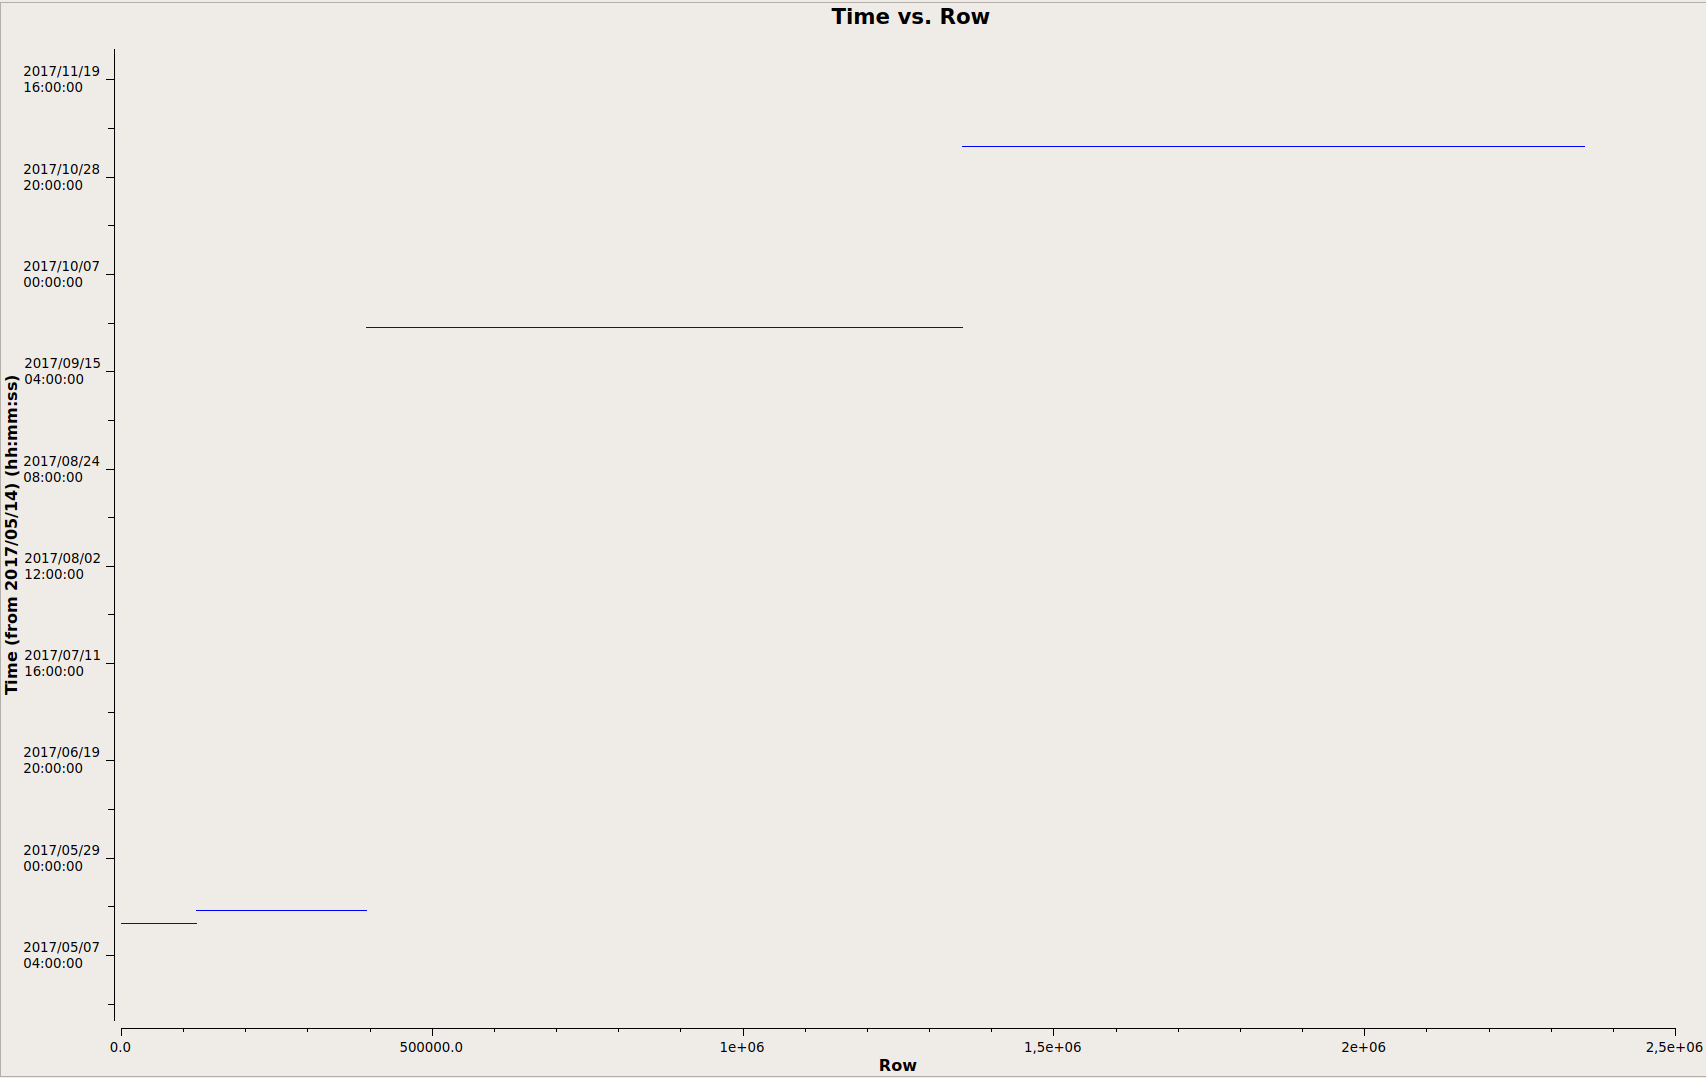
\includegraphics[scale=0.3]{images/time_vs_row.png}
	\caption[Tiempo de medición para GWLup]{Tiempo de medición para GWLup. Fuente: Elaboración propia}
	\label{fig:time_vs_row}
\end{figure}

Como se observa el tiempo aumenta pero se puede llegar a presentar ciertos cortes en los datos, esto debido al cambio de fecha de cuando se capturaron. Teniendo en cuenta esto se crea un algoritmo que agrupa los datos que estén dentro de un mismo rango de tiempo, pero en caso de presentarse un salto de tiempo como se menciona anteriormente, este no presentará un mayor problema debido a que si el rango de tiempo es lo bastante grande, el corte entrará dentro de los datos agrupados. 

El algoritmo necesita los tiempo en que fueron capturado los datos y el rango de tiempo deseado para agruparlos. La forma de realizar esto se muestra en el algoritmo \ref{alg:get_index}, donde inicialmente se define la diferencia de los tiempos para ser recorridas y un índice (denominado índice actual) que indica desde que lugar comienza y un índice final que indica en que parte termina el conjunto de datos agrupado. Luego de esto se itera hasta que el índice definido alcance el final del arreglo de las diferencias de tiempo, donde en cada iteración se ve hasta que punto los datos entran dentro del rango de tiempo y se define este límite como un índice final que será agregado a una lista de índices, además de hacer cero todos los datos que estén dentro del grupo para que no vuelvan a ser considerados. Para definir el siguiente valor del índice inicial que se evalúa en cada iteración se tienen 3 casos.

\begin{enumerate}
    \item El índice actual es igual al índice final, que es cuando solo un dato entra en el grupo, por lo que el índice actual será igual al índice final mas uno. 
    \item El índice final es igual a cero, o que quiere decir que se alcanza el final del arreglo por lo que el índice actual será igual al largo del arreglo de la diferencia de tiempos. 
    \item No se cumple ningún caso anterior por lo que el índice actual será igual al índice final. 
\end{enumerate}


\begin{algorithm}[!ht]
	\caption{Algoritmo de partición de tiempo.}
	\label{alg:get_index}
	\begin{algorithmic}[1]
	\REQUIRE Tiempo, rango de tiempo.
	\ENSURE Índices de corte. 	
	\STATE $timeDiff \gets diff(time)$
        \STATE $actualIndex  \gets 0$
        \STATE $indexList \gets [0]$

        \WHILE{$actualIndex \leq len(timeDiff) - 1$} 
            \STATE{$endIndex = (cumsum(timeDiff) \leq timeRange).argmin()$} 
            \IF {$actualIndex == endIndex$}
                \STATE $actualIndex = endIndex + 1$
            \ELSIF{$endIndex == 0$}
                \STATE $actualIndex = len(timeDiff)$
            \ELSE
                \STATE $actualIndex = endIndex$
            \ENDIF   
            \STATE $indexList.append(actualIndex)$
            \STATE $timeDiff[:actualIndex] = 0$
        \ENDWHILE 
	\RETURN $indexList$
	
	\end{algorithmic}
\end{algorithm}

En cuanto al algoritmo de \textit{self-calibration}, se debe tener en cuenta lo mencionado en optimizar la ecuación \ref{eq:self-calibration}, sin embargo en diversas implementaciones, como gaincal de CASA \citep{gaincal_task} y rascil \citep{rascil}, utilizan una variación de división de las visibilidades observadas por las modelo para encontrar el valor de las ganancias. De esta manera, se propone explorar este enfoque para el \textit{self-calibration} a implementar, donde para esto se debe tener en consideración la ecuación \ref{eq:self-calibration-3} que permite relacionar las ganancias con las visibilidades observadas y modelo, donde esta permite obtener las ganancias para la fase como amplitud.

\begin{equation}
        \sum |V_{ij} - g_{i}g_{j}^{*}\tilde{V}_{ij}|^2
        \label{eq:self-calibration}
\end{equation}

\begin{equation}
    V_{i,j,corr} = \frac{\tilde{V}_{ij}}{g_{i}g_{j}^{*}}
    \label{eq:self-calibration-3}
\end{equation}

\subsection{Fase}

Para corregir la fase con \textit{Self-calibration} es necesario comprender que las ganancias se pueden definir como indica la ecuación \ref{equation:gains}, donde el gran interés se encuentra en encontrar los ángulos ($\theta$) por pares de antenas que deben ser aplicados para corregir la fase que afecta a las visibilidades. Para esto es necesario definir la \ref{eq:self-calibration-3} junto con la expresión completa de las ganancias (ecuación \ref{equation:gains}), obteniendo así la ecuación \ref{eq:self_inicial}. 

\begin{equation}
    g_{i}g_{j}^{*} = e^{2\pi i|\theta_{i} - \theta_{j}|}
    \label{equation:gains}
\end{equation}

\begin{equation}
    V_{i,j,corr} = \frac{\tilde{V}_{ij}}{e^{2\pi i|\theta_{i} - \theta_{j}|}}
    \label{eq:self_inicial}
\end{equation}

Es posible obtener el valor para un $\theta$ asociado a una antena $i$ al comenzar a realizar operaciones sobre la ecuación \ref{eq:self_inicial}, de tal manera de dejar $\theta$ despejado. Para esto se presentan a continuación las operaciones aritméticas realizadas, partiendo por un despeje simple sobre la ecuación \ref{eq:self_inicial} dando como resultado la ecuación \ref{eq:phase1}. 

\begin{equation}
    e^{2\pi i|\theta_{i} - \theta_{j}|}= \frac{\tilde{V}_{ij}}{V_{i,j,corr}}
    \label{eq:phase1}
\end{equation}

Aún así en la ecuación \ref{eq:phase1} se tienen dos ángulos distintos ($\theta_{i}, \theta_{j}$), lo que se consideraría las incógnitas a encontrar, sin embargo se tendría dos incógnitas y una ecuación por lo que no es posible encontrar el valor para ambos ángulos. Por lo mismo, para solventar esa complicación se asume que una antena tendrá ganancia 0 y se le define como antena de referencia, por lo que solo se trabajan con visibilidades que tengan asociada esta antena. Esto permite que en la ecuación \ref{eq:phase1} desaparezca un ángulo transformándose así a la ecuación \ref{eq:phase2}.

\begin{equation}
    e^{2\pi i|\theta_{i}|}= \frac{\tilde{V}_{ij}}{V_{i,j,corr}}
    \label{eq:phase2}
\end{equation}

Como se muestra en la ecuación \ref{eq:phase3}, las ganancias pueden ser divididas en coordenadas polares y cartesianas. Esto trae consigo una ventaja ya que nos permite relacionarla con la tangente mediante la ecuación \ref{eq:phase4}, permitiendo así eliminar las amplitudes que afectan a la parte imaginaria como real. 

\begin{equation}
    e^{2\pi i|\theta_{i}|} =  cos(2 \pi \theta_i) + i  sen(2 \pi \theta_i) 
    \label{eq:phase3}
\end{equation}

\begin{align} 
Re = cos(2 \pi \theta)\\ 
Im = sen(2 \pi \theta)
\end{align}


\begin{equation}
    tg(2\pi \theta_i) = \frac{Im}{Re}
    \label{eq:phase4}
\end{equation}

Finalmente, la ecuación que permite obtener el ángulo que se debe aplicar para corregir esta dada por la ecuación \ref{eq:phase5}.

\begin{equation}
    \theta_{i} = \frac{1}{2\pi}arctg(\frac{Im}{Re})
    \label{eq:phase5}
\end{equation}

Todo lo mencionado anteriormente es combinado en un algoritmo en el cual se obtiene los ángulos para las visibilidades asociadas a la antena de referencia, se calcula los rangos de tiempo y para cada rango se realiza el promedio ponderado reemplazando los nuevos ángulos. Este se puede ver representado en el algoritmo \ref{alg:selfcalibration-impl}. Cabe destacar que dentro de este algoritmo se representa el algoritmo \ref{alg:get_index} por la función \textit{get\_index} y por otro lado la función \textit{get\_thetas} aplica la ecuación \ref{eq:phase5} mostrada anteriormente. 

\begin{algorithm}[!ht]
	\caption{Algoritmo de \textit{Self-calibration} implementado}
	\label{alg:selfcalibration-impl}
	\begin{algorithmic}[1]
	\REQUIRE Dataset en formato MS, rango de tiempo, antena de referencia.
	\ENSURE Dataset en formato MS.
	
	\FOR{$spectral\ window$}
	    \STATE $vis\_obs \gets visibilities.data$ \\
	    \STATE $vis\_mod \gets visibilities.model$ \\ 
        \STATE $weight \gets visibilities.weight$ \\
        \STATE $time \gets visibilities.time$ \\ 

        \STATE $vis\_ant\_ref \gets where(vis\_obs.antenna1 == ant\_ref\ or\ vis\_obs.antenna1 == ant\_ref)$

        \STATE $thetas \gets get\_thetas(vis\_obs, vis\_mod)$
        
        \STATE $indexs \gets get\_index(time, time\_range)$
        \FOR{ $i\ in\ len(indexs)$ }
            \STATE $slice \gets slice(indexs[i]:index[i+1])$\\

            \STATE $thetas\_ant\_ref \gets thetas[slice]$\\
            \STATE $weight\_ant\_ref \gets weight[slice]$\\

            \STATE $wheighted\_thetas \gets thetas\_ant\_ref * weight\_ant\_ref$ \\ 
            \STATE $sum\_weight \gets sum(weight\_ant\_ref)$\\
            \STATE $result \gets wheighted\_thetas / sum\_weight$\\

            \STATE $thetas[slice] \gets result$\\
        \ENDFOR 
            
        \STATE $vis\_ant\_ref \gets applycal(vis\_obs,thetas)$\\
	 
	\ENDFOR
	
	\RETURN $vis\_ant\_ref$
	
	\end{algorithmic}
\end{algorithm}

Aún así puede existir el caso donde el tiempo ingresado sea definido por 'inf', es decir, un tiempo infinito. Para solventar este caso el promedio se realiza por número de \textit{scan}, por lo que no existiría un rango de tiempo asociado sino que se promediaría por visibilidades asociadas a un \textit{scan}. La diferencia con el algoritmo \ref{alg:selfcalibration-impl} ya no estaría utilizando el algoritmo \ref{alg:get_index} y tampoco realizando la iteración por las particiones encontradas, sino que se buscaría los números de \textit{scan} asociados al conjunto de datos y se iteraría en cada uno para buscar las visibilidades asociadas para realizar el mismo promedio que se realiza en el algoritmo \ref{alg:selfcalibration-impl}.

Por otro lado, el promedio ponderado se realiza sobre los ángulos encontrados mediante la ecuación \ref{eq:phase5} y este es calculado mediante la ecuación \ref{eq:prom} que será aplicado antes de realizar el \textit{applycal}. Donde $\theta$ son los ángulos encontrados y $w$ es el peso asociado a las visibilidades asociadas a los $\theta$.

\begin{equation}
    \theta' = \frac{\sum \theta w}{\sum w}
    \label{eq:prom}
\end{equation}

La función \textit{applycal} realiza la acción de aplicar los $\theta$ encontrados a las visibilidades agrupadas, ya sea mediante rango de tiempo o \textit{scan\_number}. Para hacer esto implementa la ecuación \ref{eq:applycal}.

\begin{equation}
    V_{corr} = \frac{V_{obs}}{e^{2 \pi i \theta}}
    \label{eq:applycal}
\end{equation}

\subsection{Amplitud}

Para la realización de la calibración en amplitud se toma en consideración el análisis realizado para fase, pero la ecuación \ref{eq:phase2} se transforma en la ecuación \ref{eq:amp1}. Así también, otra diferencia a encontrar es en la función \textit{applycal} utilizada en al algoritmo \ref{alg:selfcalibration-impl}, que es dado por la ecuación \ref{eq:amp2}.

\begin{equation}
    A = \bigg|\frac{V_{obs}}{V_{mod}}\bigg| 
    \label{eq:amp1}
\end{equation}

\begin{equation}
    V_{corr} = \frac{V_{obs}}{A}
    \label{eq:amp2}
\end{equation}

Al igual que en el caso de la fase, si se ingresa un valor como 'inf' para el tiempo, se considera la utilización de las visibilidades asociadas a un número de \textit{scan} para poder realizar el promedio ponderado. 

\section{\textit{Bispectrum}}
\label{sec:bispectrum}

Para utilizar la ecuación \ref{eq:RML} mostrada en la sección \ref{subcap:sintesis} es necesario definir la ecuación a minimizar para los datos del modo bispectrum, para estos se utilizará la definida en el articulo \cite{Chael_2018}. Este define la ecuación \ref{eq:bispectrum_2}. 

\begin{equation}
    \chi^{2}_{bispec}(I) = \frac{1}{2N_{B}} \sum_{j} \frac{| V_{Bj}  - V'_{Bj}|^2}{\sigma^{2}_{Bj}}
    \label{eq:bispectrum_2}
\end{equation}

Donde $V_{Bj}$ corresponde a las visibilidades observadas de $I$ en formato \textit{Bispectrum}, $N_{B}$ corresponde a la cantidad de medidas \textit{Bispectrum}, $V'_{Bj}$ corresponde a las visibilidades observadas en formato \textit{Bispectrum} y $\sigma^{2}_{Bj}$ corresponde a la varianza estimada. Para calcular este último es necesario utilizar la ecuación \ref{eq:sigma}.

\begin{equation}
    \sigma_{B} = |V_{B}| \sqrt{\frac{\sigma^{2}_{1}}{|V_{1}|^{2}} + \frac{\sigma^{2}_{2}}{|V_{2}|^{2}} + \frac{\sigma^{2}_{3}}{|V_{3}|^{2}}}
    \label{eq:sigma}
\end{equation}

Para obtener los datos necesarios en las ecuaciones anteriores se realiza la creación de un algoritmo que busca las posibles combinaciones de tres que se pueden realizar con las antenas disponibles y calcular los pesos mediante la ecuación \ref{eq:sigma} para todos los datos. Luego de esto se busca las visibilidades observadas, modelos y los pesos relacionadas a la combinación de antenas. El algoritmo que muestra este proceso se puede ver en el algoritmo \ref{alg:bispectrum}.

Cabe destacar que se debe tener en cuenta la cantidad de antenas que tiene el conjunto de datos debido a que los números de combinaciones posibles para tríos de antenas son muchos, por ejemplo, para un observatorio como ALMA que tiene 66 antenas \citep{antenas_alma} se tendría un total de 45760 combinaciones posibles. Para esto, como se utilizó en \citet{Chael_2018}, se toma una antena de referencia que permite disminuir la cantidad de combinaciones posibles y por ende el tiempo de ejecución del método, donde si se toma el ejemplo anterior se tiene que la cantidad posible de combinaciones con una antena de referencia disminuye a 2080. 

\begin{algorithm}[!ht]
	\caption{Algoritmo de Bispectrum.}
	\label{alg:bispectrum}
	\begin{algorithmic}[1]
    \REQUIRE Conjunto de datos (MS), antena de referencia.
    \ENSURE Conjunto de datos reordenado	
    \STATE $unique\_time \gets unique(visibilities.time)$
    \STATE $antennas \gets visibilities.antenna$
    \STATE $combs \gets combination(visibilities.antennas)$
    \STATE $filt\_combs \gets [x\ for\ x\ in\ combs\ if\ ant\_ref\ in\ x]$
    \STATE $n\_comb \gets filt\_combs.size$
    \STATE $n\_utime \gets unique\_time.size$
    \STATE $nchan, ncorr \gets visibilities.shape$
    \STATE $count  \gets zeros\_like((n\_comb, n\_utime, 3, nchan, ncorr))$
    \STATE $bis\_data \gets zeros\_like((n\_comb, n\_utime, 3, nchan, ncorr))$

    \FOR{$row\ in\ visibilities$}

        \FOR{$ic, comb\ in\ filter\_combs$}
        \STATE $utime \gets unique\_time[row]$
        \STATE $antenna1 \gets antennas[row][0]$
        \STATE $antenna2 \gets antennas[row][1]$

        \IF{$antenna1 == comb[0] \ and\ antenna2 == comb[1]$}
            \STATE $bis\_data[comb, utime, 0] = visibilities[row] $
            \STATE $count[comb, utime, 0] += 1 $
        \ELSIF{$antenna1 == comb[1] \ and\ antenna2 == comb[-1]$}
            \STATE $bis\_data[comb, utime, 1] = visibilities[row] $
            \STATE $count[comb, utime, 1] += 1 $
        \ELSIF{$antenna1 == comb[0] \ and\ antenna2 == comb[-1]$}
            \STATE $bis\_data[comb, utime, 2] = visibilities[row] $
            \STATE $count[comb, utime, 2] +=  1$
        \ENDIF
    \ENDFOR

    \ENDFOR

    \STATE $bis\_data[count != 3] = 0$
    
    \RETURN $bis\_data$
	
	\end{algorithmic}
\end{algorithm}

En el algoritmo \ref{alg:bispectrum} se muestra lo implementado para el ordenamiento de los datos para luego ser calculados en el formato \textit{Bispectrum}. Inicialmente se definen las antenas y sus combinaciones de tríos filtrados por una antena de referencia, además de definir los tiempos de las visibilidades para poder ordenarlas y un contador para ver las visibilidades que cumplen con el requisito de formar un triangulo. 

Luego de definir estas variables se recorre cada visibilidad y dentro de cada iteración se recorre las combinaciones filtradas. En cada iteración para las combinaciones se verifica en que posición de la combinación está el par de antenas asociado a la visibilidad, es decir, si es $ij$, $jk$ o $ki$ y según esto se ingresa a su posición respectiva en el arreglo de datos \textit{bispectrum}, además de sumarse uno al arreglo de contador para que finalmente todas las combinaciones en que su conteo no de igual a 3 se eliminan porque sus antenas no forman un triangulo.  

El guardado de los datos en su formato \textit{Bispectrum} debe tener en consideración que la información original debe mantenerse, por lo mismo los datos calculados son almacenados en otra columna. Esta contiene unas dimensiones distintas a las visibilidades originales, donde estas son (ncomb, nutime, nant, nchan, ncorr). Cada una de estas dimensiones significa lo siguiente.

\begin{itemize}
    \item \textbf{ncomb}: Indica a que combinación de tríos de antenas pertenece las visibilidades. 
    \item \textbf{nutime}: Indica en que tiempo único se realizo la medición. Esto permite agrupar aquellas visibilidades que se obtuvieron en el mismo instante.    
    \item \textbf{nant}: Este indica a que combinación de antenas pertenece la visibilidad, es decir, si pertenece a la combinación $ij$, $jk$ ó $ki$. 
    \item \textbf{nchan}: Al igual que las visibilidades originales, este representa la cantidad de canales de las visibilidades. 
    \item \textbf{ncorr}: Al igual que las visibilidades originales, este reprenta la cantidad de correlaciones de las visibilidades.  
\end{itemize}

Sin embargo, almacenado de esta manera no se puede considerar que este en su formato \textit{Bispectrum} debido a que solo se reorganiza el conjunto de datos y no se realiza el calculo de la ecuación \ref{eq:bispectrum} para las visibilidades, ni la ecuación \ref{eq:sigma} para los pesos. La ventaja de la dimensión \texttt{nant} es que permite realizar la multiplicación en este eje de tal manera de cumplir con las ecuaciones anteriores conllevando a que la dimensión final sea (ncomb, nutime, nchan, ncorr). 

Otros datos también son guardados para complementar la información anterior, entre lo que se encuentra las antenas correspondiente al trió construido y las posiciones $uvw$ para cada visibilidad.  

\subsection{Gradiente conjugado}

Para obtener la solución necesaria para el \textit{Bispectrum} se debe implementar un método para minimizar la ecuación \ref{eq:bispectrum}, el cual para este caso se utiliza el gradiente conjugado. Para esto se calcula el gradiente de la ecuación \ref{eq:bispectrum} que está dada por la ecuación \ref{eq:derivadaBis}, donde el análisis y pasos para llegar a este están explicadas en el Apéndice \ref{finales:apendice1}.

\begin{equation}
    \begin{split}
        \frac{\partial{\chi^{2}_{bis}}}{\partial_{I_{k}}} &= \frac{-1}{N_{B}} \sum_{j} \frac{1}{\sigma^{2}_{Bj}} Re\bigg((V_{Bj} - V'_{Bj}) \bigg( \frac{\partial{V'_{Bj}}}{\partial{I_{k}}} \bigg)^{*} \bigg) \\
        &= \frac{-1}{N_{B}} \sum_{j} \frac{1}{\sigma^{2}_{Bj}} Re\bigg((V_{Bj} - V'_{Bj}) V^{'*}_{Bj} \bigg( \frac{e^{2\pi i (u_{1j}x_{k} + v_{1j}y_{k})}}{V^{'*}_{1j}} + \frac{e^{2\pi i (u_{2j}x_{k} + v_{2j}y_{k})}}{V^{'*}_{2j}} + \frac{e^{2\pi i (u_{3j}x_{k} + v_{3j}y_{k})}}{V'^{'*}_{3j}}\bigg) \bigg) 
    \end{split}
    \label{eq:derivadaBis}
\end{equation}

Un método que permite la optimización de la ecuación \ref{eq:derivadaBis} es el método del gradiente conjugado no lineal. El algoritmo \ref{alg:nolinealgradient} presenta la implementación de este método, donde se debe tener en consideración que este necesita una imagen inicial representada por $x$, un método de búsqueda lineal que es un objeto que tendrá dentro una función objetivo a minimizar, la cantidad total de iteraciones a realizar, un error asociado para el criterio de parada, un epsilon y una máscara que permite la optimización y calculo solo en un sector de la imagen. Finalmente este retorna la imagen optima encontrada. 

\begin{algorithm}[!ht]
	\caption{Algoritmo de Gradiente conjugado no lineal}
	\label{alg:nolinealgradient}
	\begin{algorithmic}[1]
	\REQUIRE Imagen, Método de búsqueda lineal, iteraciones, error, epsilon, máscara. 
	\ENSURE Gradiente de $f$. 

    \STATE $obj\_func \gets linmin.objective\_function$
    \STATE $f_{k} \gets obj\_function.calculate\_function(mask)$
    \STATE $d_{k} \gets obj\_function.calculate\_gradient(mask)$
	
	\FOR{\textit{iterations}} 
        \STATE $step \gets linmin.search(mask)$
        \STATE $x_{k+1} \gets x_{k} - step * d_{k}$
        \STATE $f_{k+1} \gets f(x_{k+1})$

        \IF{$2(f_{k+1} - f_{k}) <= error(abs(f_{k+1}) + abs(f_{k}) * epsilon)$}
         \RETURN $f'_{k+1}$
        \ENDIF

        \STATE $f_{k} \gets f_{k+1}$
        \STATE $\beta \gets rebiere\_polyak()$
        \STATE $d_{k} \gets -d_{k} + \beta d_{k-1}$
	\ENDFOR
	
	\RETURN $f'_{k+1}$
	
	\end{algorithmic}
\end{algorithm}

La búsqueda lineal es un objeto de Pyralysis que, como se mencionó anteriormente, contiene un objeto de función objetivo y permite la búsqueda del mejor paso (\textit{step}) para el gradiente. Los métodos implementados de búsqueda lineal son \textit{Backtracking} con la regla de Armijo, el método de \textit{Fixed Step} y  el método de \textit{Brent} sin embargo este último es el utilizado para las pruebas.  

El criterio de parada para el gradiente esta dada por la ecuación \ref{eq:stop_crit}. Este permite un criterio de parada más preciso sin decaer en realizar iteraciones innecesarias, además se agrega un error $\epsilon$ para evitar una división por cero. 

\begin{equation}
    \label{eq:stop_crit}
    \frac{ 2*|f_{k+1} - f_{k}|}{|f_{k+1} + f_{k}| + \epsilon}\leqslant error  
\end{equation}

Por otro lado, en la línea 12 del algoritmo \ref{alg:nolinealgradient} se menciona el calculo de un $\beta$, el cual es utilizado para obtener la nueva dirección de desplazamiento $d_{k}$. Para calcular este se utiliza el método de Polak-Ribiere-Polyak que define el valor de $\beta$ por la ecuaciíon \ref{eq:rebiere_polyak}.

\begin{equation}
    \label{eq:rebiere_polyak}
    \beta = \frac{g^{T}_{k}(g_{k} - g_{k-1})}{||g_{k-1}||^{2}}
\end{equation}


\begin{comment}
\section{Antena de referencia}

En los análisis de \textit{self-calibration} y \textit{Bispectrum} se ha mencionado el uso de una antena de referencia que ayuda de manera especifica en cada uno de los métodos. Sin embargo, una buena elección de esta es importante debido a que una mal antena seleccionada puede traer a un resultado erróneo. Lo ideal es que la antena de referencia sea una ubicada al centro del conjunto de antenas asociada al conjunto de datos.
\end{comment}


\section{Creación de datos simulados}
\label{sec:simulated_data}

Para comprobar la eficacia de los métodos implementados se necesita de un conjunto de datos controlado. Es así que se realiza la creación de un conjunto de datos simulado, o también llamado híbrido, por su combinación de información simulada y real. El proceso para esto se basa en lo propuesto en el trabajo de \citet{FernandezTesis}, por lo que se presentan aquellos aspectos que son similares. El proceso general de este es el siguiente.

\subsection{Conjunto de datos reducidos}
\label{sec:datos_reducidos}

Las alteraciones atmosféricas son variantes durante el tiempo y al ser estás las causantes de las perturbaciones en los datos se puede considerar que esta perturbación no será igual de un día para otro. Esto conlleva a que se debe disminuir el conjunto de datos a trabajar al tiempo de medición mas pequeño, de tal manera de obtener la menor variación en las perturbaciones de los datos. 

Para la creación de este conjunto de datos reducido se utiliza como inicial el obtenido a través del conjunto de datos HD163296, el cual se encuentra público en el sitio web de DSHARP. A través del uso de TaQL se puede obtener el rango de tiempo de medición junto a la cantidad de observaciones asociadas a este tiempo, de tal manera que un resumen de estos datos se puede ver en la Tabla \ref{tab:observations}. 

\begin{table}[!ht]
	\begin{center}
		\caption{Tabla con cantidad de observaciones para HD163296.}
		\begin{tabular}{| c | c | c | c | c | c |}
			\hline
			  ID observación & Fecha Inicio & Inicio & Fin & Duración & Observaciones\\ \hline
			0 & 04/06/2014 & 07:20:48 & 08:23:21 & 01:02:23 & 97522\\ \hline
            1 & 14/06/2014 & 06:30:15 & 07:32:28 & 01:02:13 & 111589\\ \hline
            2 & 16/06/2014 & 07:19:21 & 08:21:17 & 01:01:56 & 86139\\ \hline
            3 & 17/06/2014 & 07:52:13 & 08:37:14 & 00:47:01 & 58634\\ \hline
            4 & 29/06/2014 & 05:56:42 & 07:01:49 & 01:05:07 & 94778\\ \hline
            5 & 05/08/2015 & 04:34:01 & 05:43:25 & 01:29:45 & 126787\\ \hline
            6 & 08/08/2015 & 03:50:19 & 05:00:21 & 01:01:02 & 156090\\ \hline
            7 & 09/08/2015 & 01:01:41 & 02:31:28 & 01:29:47 & 50458\\ \hline
            8 & 08/09/2017 & 22:30:25 & 23:06:21 & 00:36:06 & 589711\\ \hline
            9 & 08/09/2017 & 23:29:08 & 00:27:04 & 00:57:56 & 1022112\\ \hline
		\end{tabular}
		\label{tab:observations}
	\end{center}
	\begin{center}
		Fuente: Elaboración propia.
	\end{center}
\end{table}

Si se ve los datos de la tabla \ref{tab:observations} se puede observar que la observación con id 8 la cual tiene una duración de 36 minutos con 6 segundos y un total de observaciones de 589711, es la apropiada para reducir el conjunto de datos debido a que tiene la ventana de tiempo mas pequeña y las variaciones en las perturbaciones de esta no deberían ser muy significativas. De esta manera el nuevo conjunto de datos a crear será seleccionando las visibilidades asociadas a la observación seleccionada. 

Sin embargo, la observación elegida anteriormente corresponde a aquellas capturadas a través de \textit{long-baseline} por lo que es necesario la creación de un conjunto de datos capturados a través de \textit{short-baseline}. Para esto se utiliza el mismo conjunto de datos HD163296 y se debe tener en consideración que de la tabla \ref{tab:observations} las observaciones con id desde 0 a 7 corresponden a \textit{short-baseline} y las otras corresponden a \textit{long-baseline}. De esta manera se realiza la elección de la observación con id 3, que tuvo una duración de 47 minutos con 1 segundo y contiene 85139 visibilidades, debido a que su ventana de tiempo es la mas corta. 


\subsection{Imagen sucia a conjunto de datos reducido}
\label{subsec:dirty_image}

Obtenido el nuevo conjunto de datos reducido se puede crear la imagen sucia de este que servirá para procesos posteriores. Esta se crea a través de \texttt{tclean} ofrecido por el framework CASA donde el resultado final para la observación con \textit{long-baseline} puede verse en la Figura \ref{fig:hd163296_obs8} y la observación con \textit{short-baseline} puede ser vista en la Figura \ref{fig:hd163296_obs3}. 

\begin{figure}[!ht]
 \centering
  \subfloat[Colores originales]{
   \label{fig:original_color}
    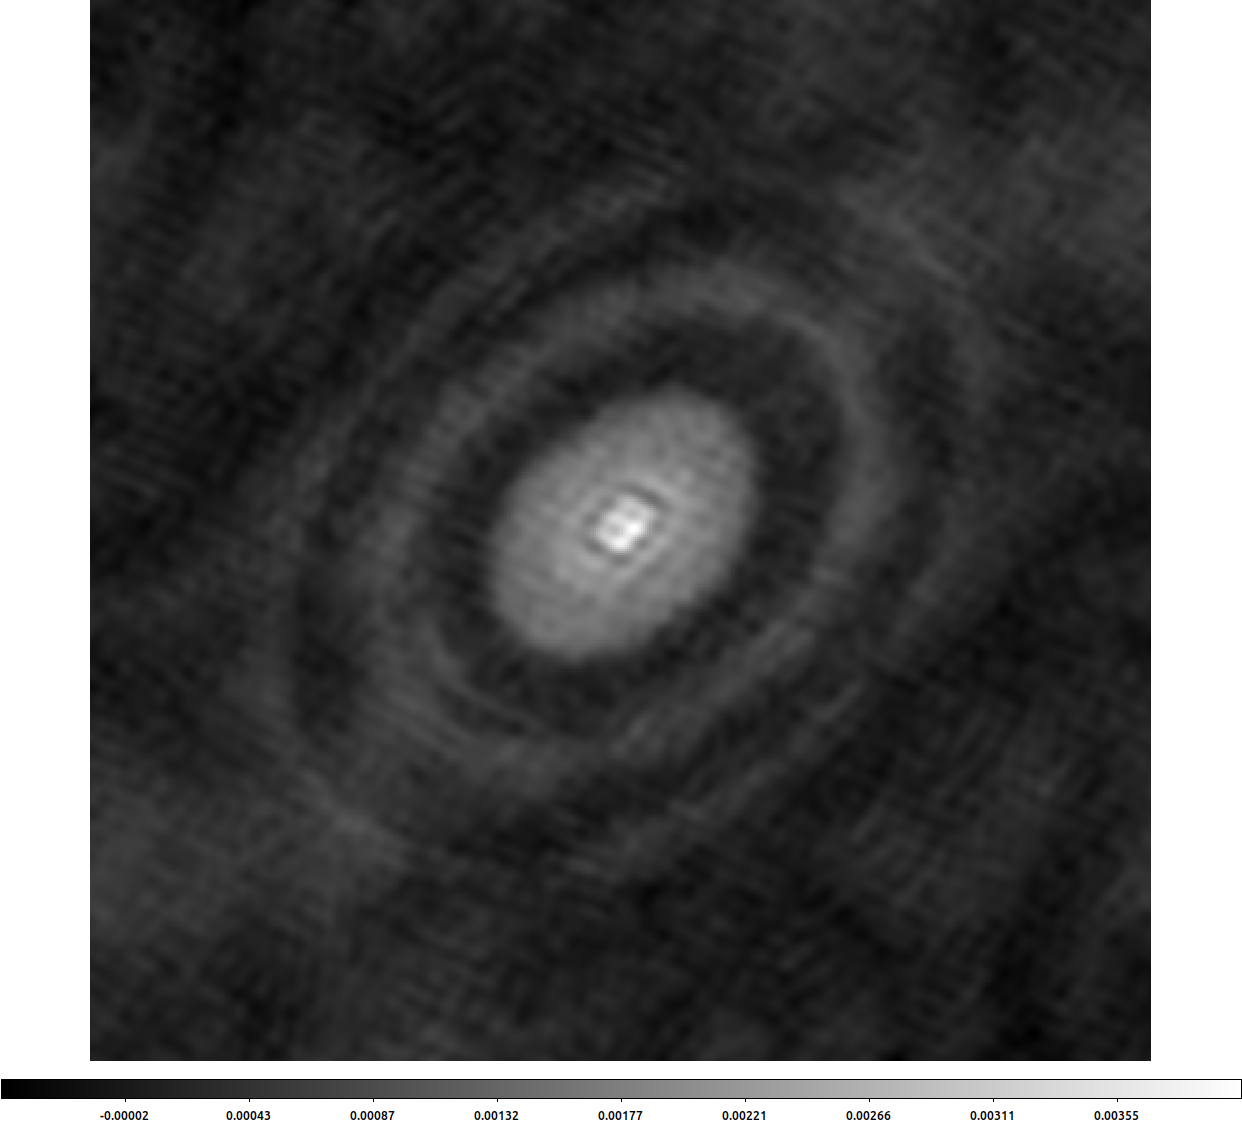
\includegraphics[width=0.45\textwidth]{images/HD163296_short8.png}}
  \subfloat[Colores artificiales]{
   \label{fig:sim_color}
    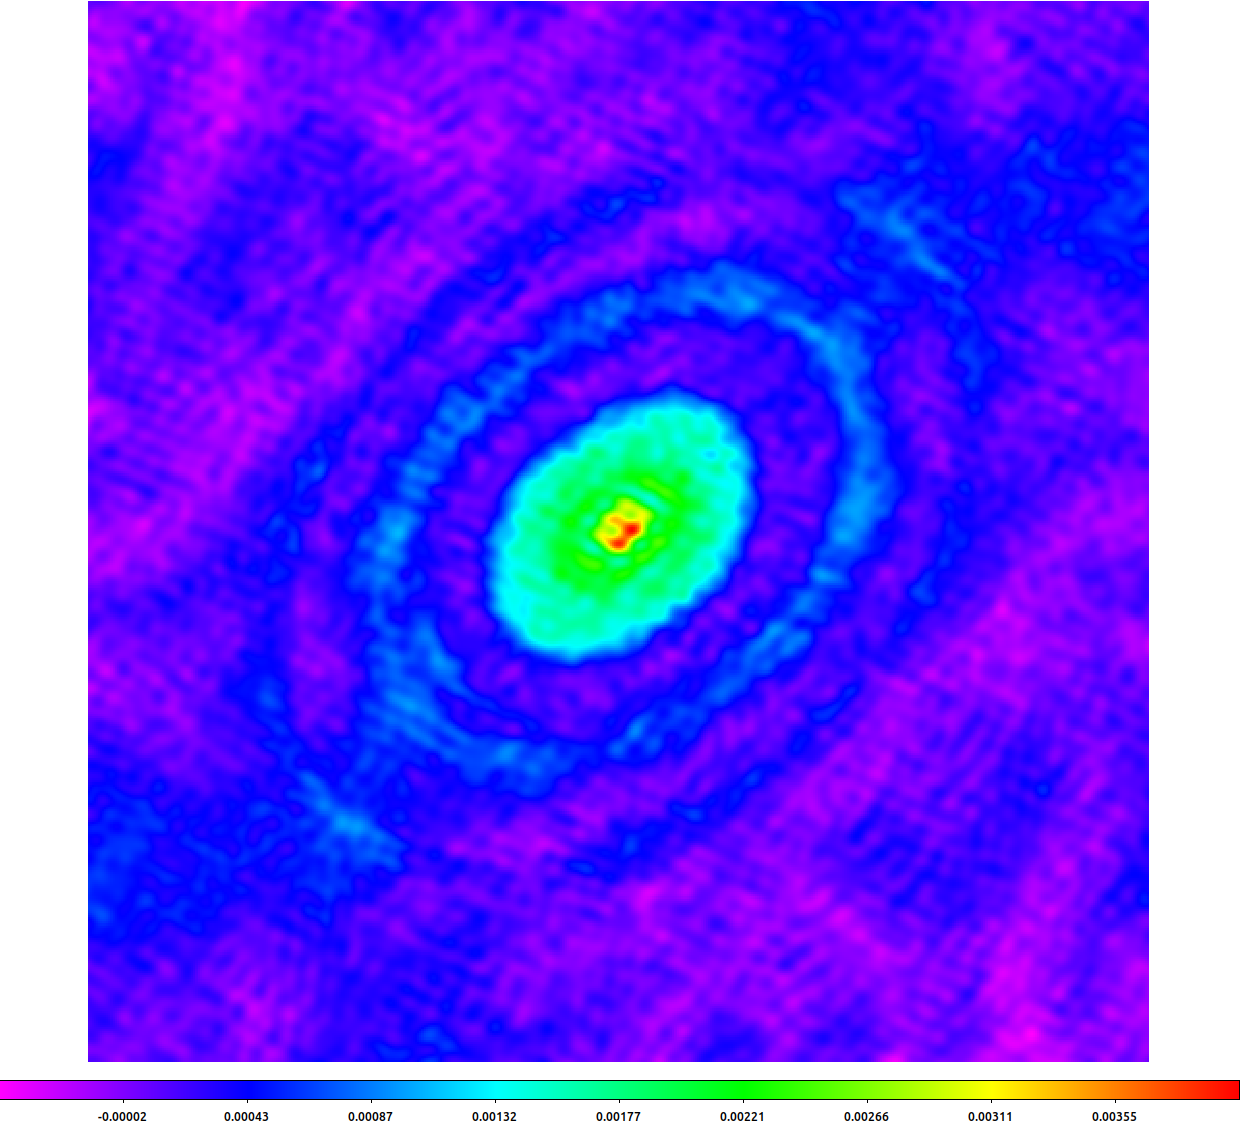
\includegraphics[width=0.45\textwidth]{images/HD163296_short8_colors.png}}
 \caption[Imagen sucia de HD163296 reducido (\textit{long-baseline})]{Imagen sucia de HD163296 reducido (\textit{long-baseline}). Fuente: Elaboración propia.}
 \label{fig:hd163296_obs8}
\end{figure}

\begin{figure}[!ht]
 \centering
  \subfloat[Colores originales]{
   \label{fig:short_base_original}
    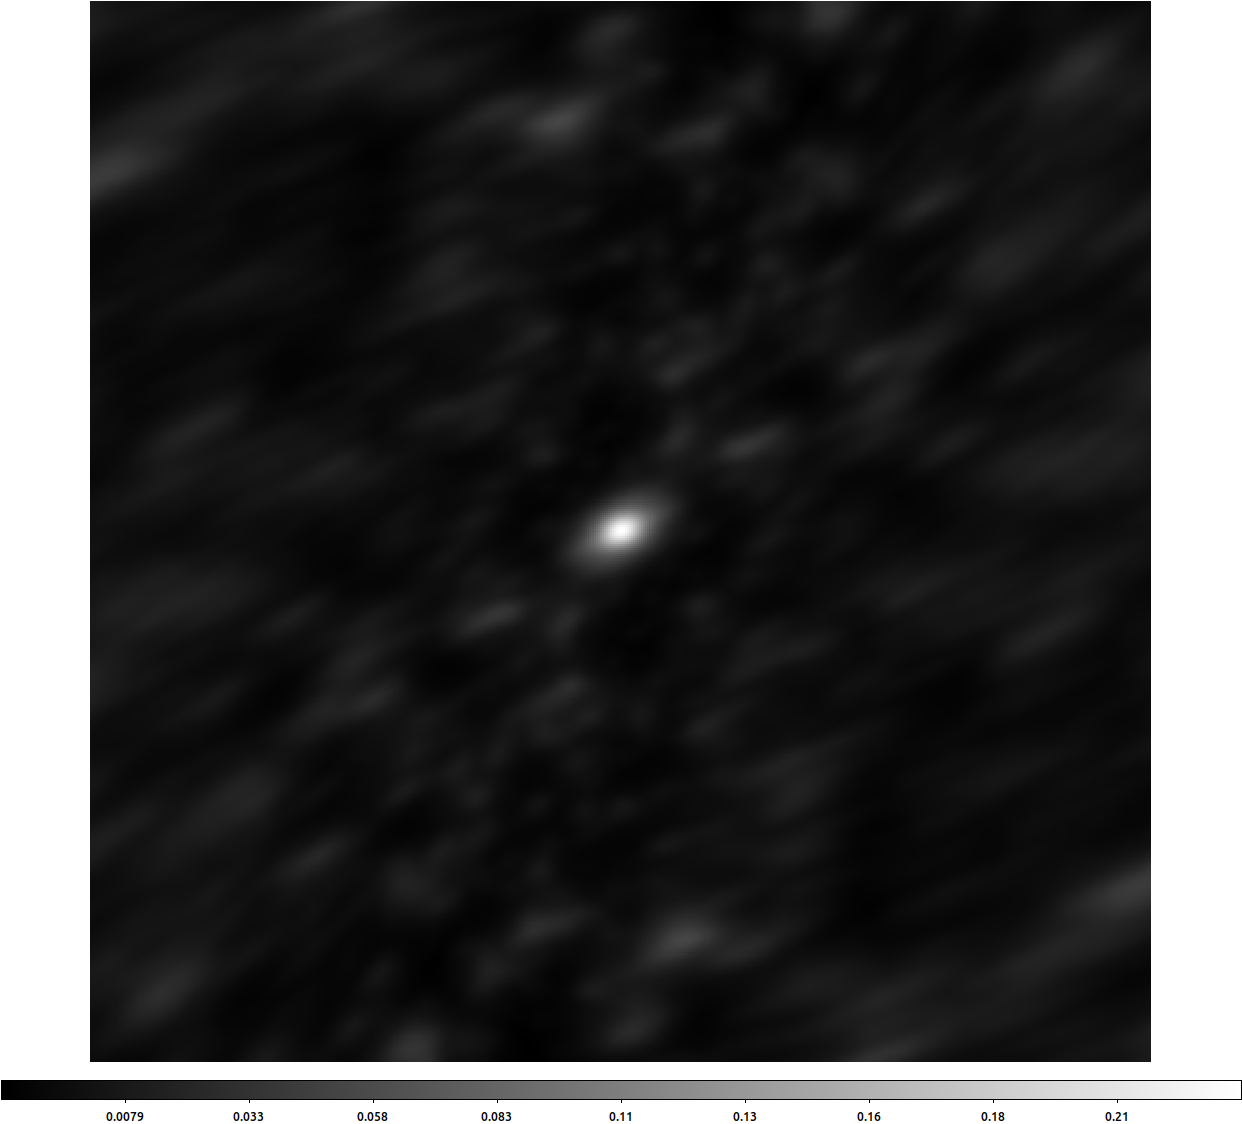
\includegraphics[width=0.45\textwidth]{images/short_base_obs3.png}}
  \subfloat[Colores artificiales]{
   \label{fig:short_base_color}
    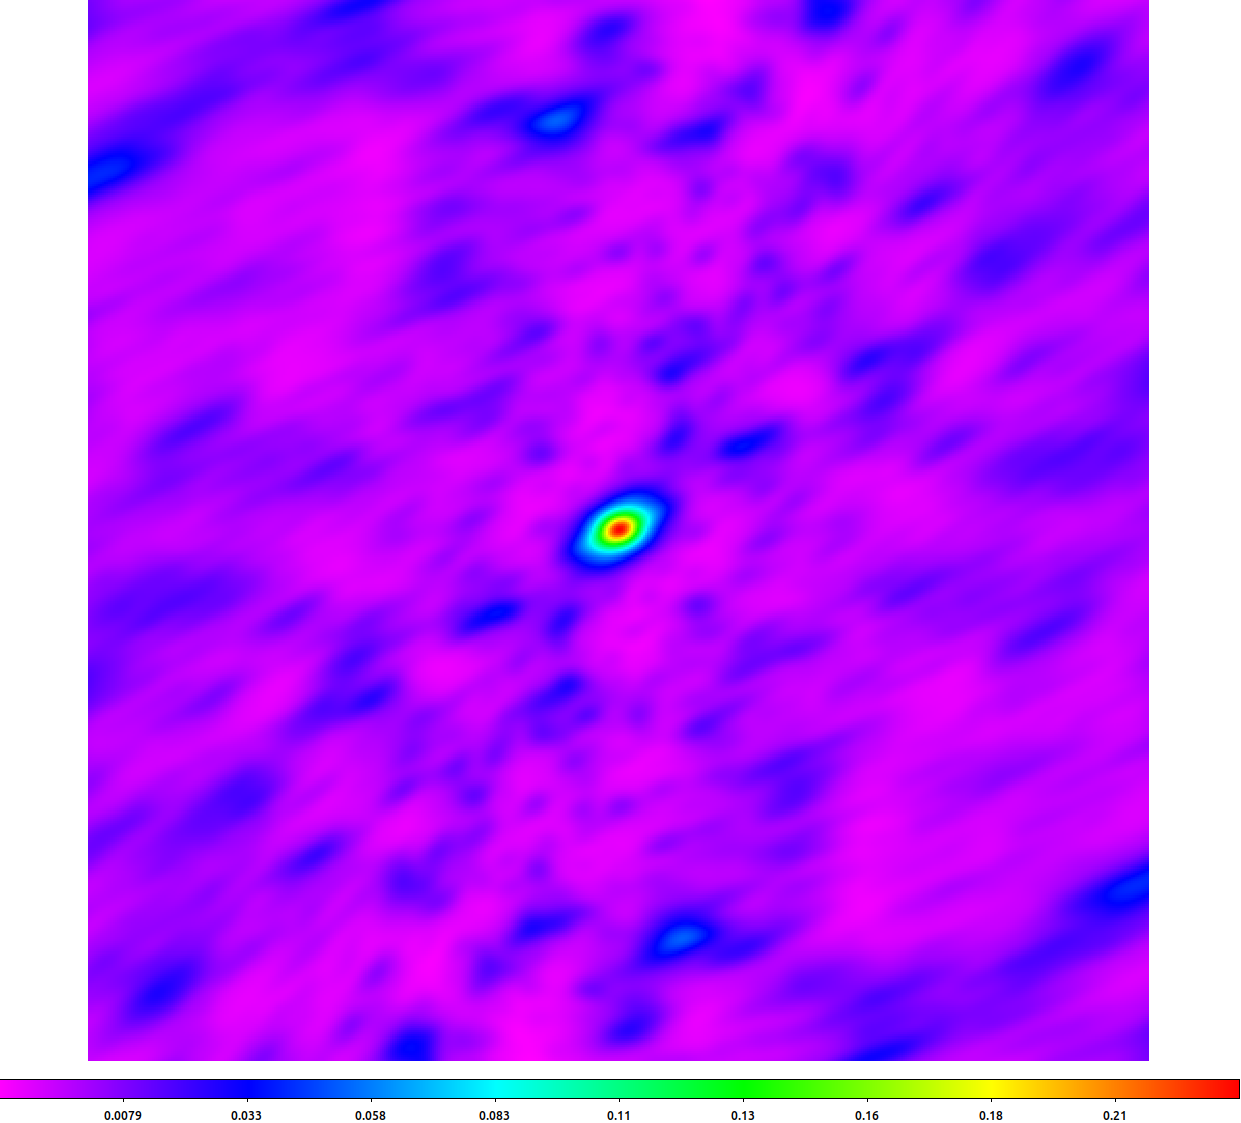
\includegraphics[width=0.45\textwidth]{images/short_base_obs3_color.png}}
 \caption[Imagen sucia de HD163296 reducido (\textit{short-baseline})]{Imagen sucia de HD163296 reducido (\textit{short-baseline}). Fuente: Elaboración propia.}
 \label{fig:hd163296_obs3}
\end{figure}


\subsection{Imagen artificial}
\label{subsec:artificial_image}

Una imagen de un objeto astronómico artificial es creada a través de un script en el lenguaje de programación \texttt{Python}. Esta imagen se encuentra en un formato FITS con un tamaño de 512x512 y será utilizada como si fuera el objeto a calibrar, es decir, como si fuera un objeto existente en el espacio exterior. La Figura \ref{fig:simulated_image} muestra la forma de este objeto donde cabe destacar que el \textit{header} de está imagen FITS es distinto según sea \textit{short-baseline} o \textit{long-baseline}. 

\begin{figure}[!ht]
	\centering
	\captionsetup{justification=centering}
	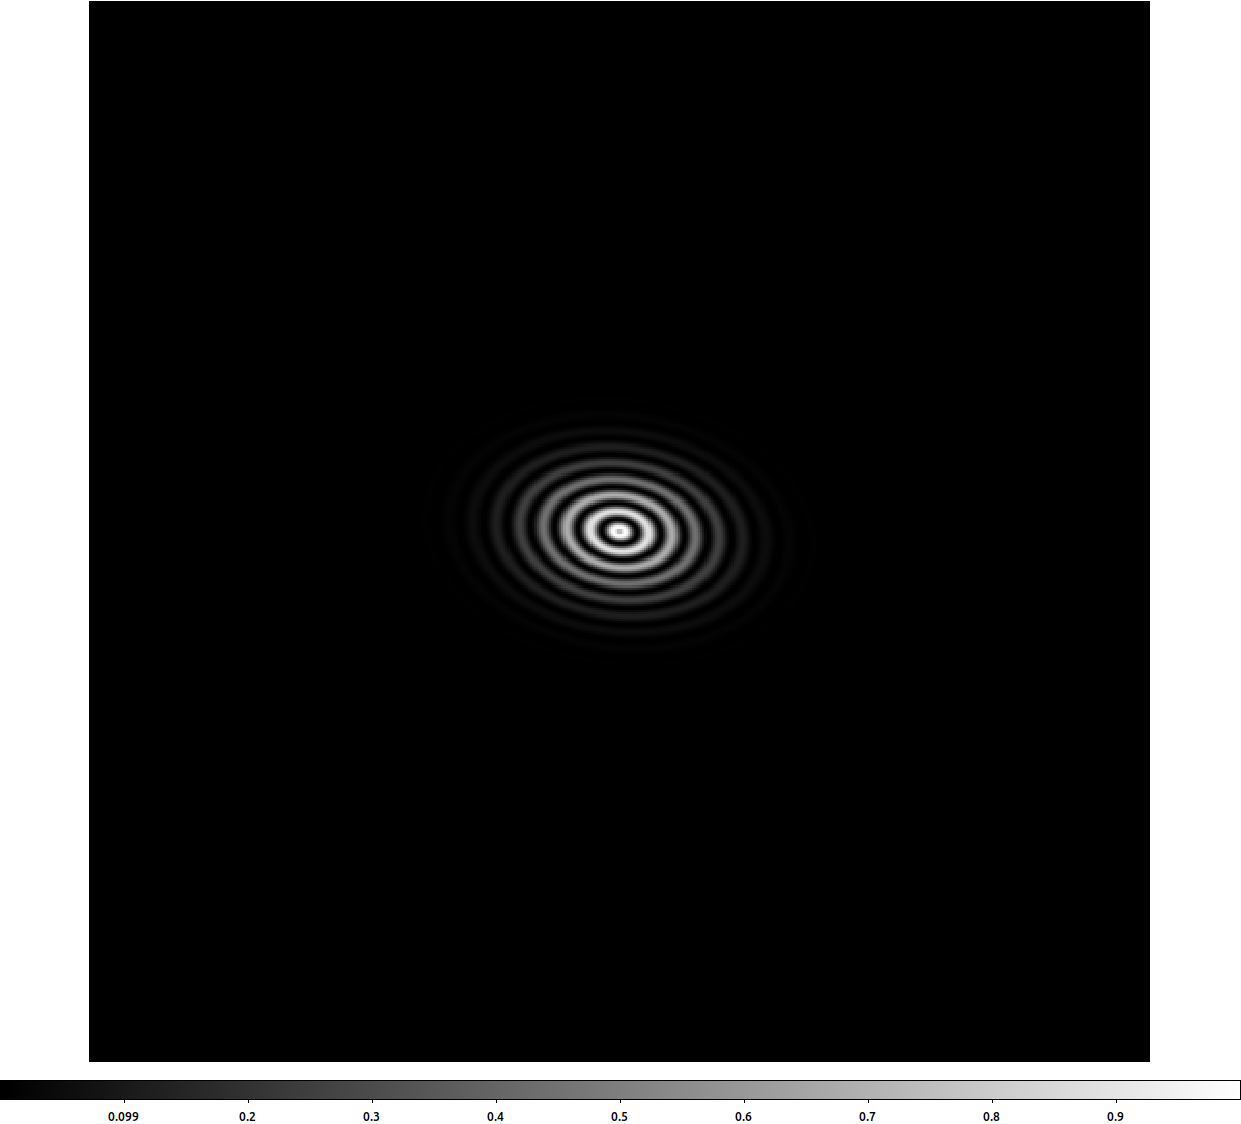
\includegraphics[scale=0.35]{images/simulated_image.png}
	\caption[Imagen artificial]{Imagen artificial. Fuente: Elaboración propia}
	\label{fig:simulated_image}
\end{figure}

\subsection{Conjunto de datos simulado}

Finalmente para crear el conjunto de datos simulado se necesita principalmente la imagen sucia creada en \ref{subsec:dirty_image} y la imagen artificial creada en \ref{subsec:artificial_image}. Obtenido esto se debe realizar los siguientes pasos. 

\begin{enumerate}
    \item Crear una imagen artificial, del tipo FITS, que contenga el \textit{Header} del conjunto de datos reducido de HD163296 y los datos de la imagen artificial. Este script puede ser visto en el Apéndice \ref{finales:apendice4}. 
    \item A través del comando \texttt{imporfits} del framework CASA, la imagen artificial anterior se convierte de su formato FITS a un formato Image. 
    \item Utilizando el comando \texttt{ft} del framework CASA se puede ingresar una columna modelo hacia un conjunto de datos. De esta manera la conjunto de datos reducido de HD163296 se le ingresa una columna modelo utilizando la imagen artificial en formato Image creada en el paso anterior. 
    \item Finalmente, la creación de un nuevo conjunto de datos puese ser lograda a través del comando \texttt{mstransform} del framework CASA. Este permite intercambiar la columna MODEL con la columna DATA, de tal manera de que la información de la imagen artificial sea la presente en el conjunto de datos creado. 
\end{enumerate}

De esta manera se obtiene un nuevo conjunto de datos que contiene visibilidades simuladas pero con la demás información como cantidad de antenas, tiempo de observación, pesos, entre otros, es parte del conjunto de datos reducido HD163296. Los comandos utilizados en los pasos 2,3 y 4, junto a los parámetros utilizados en estos pueden ser encontrados en el Apéndice \ref{finales:apendice5}. 
%\chapter{Self-calibration}
\label{cap:selfcalibration}

\begin{comment}
La síntesis de imágenes en radio-interferometría permite generar mapas (imágenes) de ondas de radio emitidas del cielo, las cuales son capturadas por un conjunto de antenas. Sin embargo, estos datos son corrompidos por distintos factores como las distorsiones atmosféricas. Este ruido se presenta como un factor complejo y constante que multiplica la señal recibida de cada antena. Sin embargo, el proceso de auto-calibracion o \textit{self-calibration} permite disminuir este factor, o también denominado ganancias, a través de un ciclo iterativo donde se crea una imagen con los datos actuales, se encuentra las ganancias asociadas a esta y se dividen los datos por las ganancias estimadas, volviendo al paso de generación de imagen de ser necesario. Aunque en el primer paso de \textit{self-calibration} se considere la síntesis de imágenes, este en si es un problema indeterminado o mal puesto debido a que la transformación que va desde el plano de la imagen hasta los datos es altamente no invertible, por lo que una infinidad de imágenes cumple con los datos recibidos. Sin embargo, existen métodos que permiten la generación del mapa como CLEAN o MEM pero son altamente sensibles al factor multiplicativo. Aunque una técnica reciente denominada \textit{bispectrum} permite generar mapas de los datos sin verse afectado por el factor multiplicativo, siendo una posible alternativa para efectuar el proceso de calibración. En este trabajo se propone efectuar una calibración mediante \textit{self-calibration} y síntesis de imágenes utilizando \textit{bispectrum} además de otras regularizaciones. Esto con el objetivo de responder la pregunta si el método de \textit{bispectrum} es la mejor opción para calibrar. Para esto se experimenta con diferentes simulaciones de datos, imágenes y métodos de síntesis para comparar y evaluar quien genera la mejor calibración. 
\end{comment}


Para la implementación de \textit{Self-calibration}  se probaron dos métodos para analizar cual es la mejor alternativa . El primero consiste en, como dice la literatura, optimizar la ecuación \ref{eq:self-calibration} para obtener el valor de las ganancias, para esto se aplico el método del gradiente conjugado el cual permite obtener un mínimo de la ecuación que se le entrega. Sin embargo, por el comportamiento periodico de las ganancias esté método no fue efectivo debido a que el resultado fue 

El segundo método consiste en realizar una aproximación de las ganancias mediante una división de visibilidades. Este se basa en la ecuación \ref{eq:self-calibration-3} que permite relacionar las ganancias a obtener con las visibilidades observadas y las modelo, donde además esta permite la obtención tanto para fase como amplitud.

\begin{equation}
    V_{i,j,corr} = \frac{\tilde{V}_{ij}}{g_{i}g_{j}^{*}}
    \label{eq:self-calibration-3}
\end{equation}

\section{Fase}

Para corregir la fase en \textit{Self-calibration} es necesario comprender que las ganancias se pueden definir como indica la ecuación \ref{equation:gains}, donde el gran interés se encuentra en encontrar los ángulos ($\theta$) por pares de antenas que deben ser aplicados para corregir la fase que afecta a las visibilidades. Para esto es necesario definir la \ref{eq:self-calibration-3} junto con la expresión completa de las ganancias, obteniendo así la ecuación \ref{eq:self_inicial}. 

\begin{equation}
    g_{i}g_{j}^{*} = e^{2\pi i|\theta_{i} - \theta_{j}|}
    \label{equation:gains}
\end{equation}

\begin{equation}
    V_{i,j,corr} = \frac{\tilde{V}_{ij}}{e^{2\pi i|\theta_{i} - \theta_{j}|}}
    \label{eq:self_inicial}
\end{equation}

Es posible obtener el valor para un $\theta$ asociado a una antena $i$ al comenzar a realizar operaciones sobre la ecuación \ref{eq:self_inicial}, de tal manera de dejar $\theta$ despejado. Para esto se presentan a continuación las operaciones aritméticas realizadas, partiendo por un despeje simple sobre la ecuación \ref{eq:self_inicial} dando como resultado la ecuación \ref{eq:phase1}. 

\begin{equation}
    e^{2\pi i|\theta_{i} - \theta_{j}|}= \frac{\tilde{V}_{ij}}{V_{i,j,corr}}
    \label{eq:phase1}
\end{equation}

Aún así en la ecuación \ref{eq:phase1} se tienen dos ángulos distintos ($\theta_{i}, \theta_{j}$), lo que se consideraría las incógnitas a encontrar, sin embargo se tendría dos incógnitas y una ecuación por lo que no es posible encontrar el valor para ambos ángulos. Por lo mismo, para solventar esa complicación se asume que una antena tendrá ganancia 0 y se le define como antena de referencia por lo que solo se trabajan con visibilidades que tenga asociada esta antena. Esto permite que en la ecuación \ref{eq:phase1} desaparezca un ángulo transformándose así a la ecuación \ref{eq:phase2}.

\begin{equation}
    e^{2\pi i|\theta_{i}|}= \frac{\tilde{V}_{ij}}{V_{i,j,corr}}
    \label{eq:phase2}
\end{equation}

Como se muestra en la ecuación \ref{eq:phase3} esta puede ser dividida en coordenadas polares y cartesianas. Esto trae consigo una ventaja ya que nos permite relacionarla con la tangente mediante la ecuación \ref{eq:phase4}, permitiendo así también permitirnos eliminar las amplitudes que afectan a la parte imaginaria como real. 

\begin{equation}
    e^{2\pi i|\theta_{i}|} =  cos(2 \pi \theta_i) + i  sen(2 \pi \theta_i) 
    \label{eq:phase3}
\end{equation}

\begin{align} 
Re = cos(2 \pi \theta)\\ 
Im = sen(2 \pi \theta)
\end{align}


\begin{equation}
    tg(2\pi \theta_i) = \frac{Im}{Re}
    \label{eq:phase4}
\end{equation}

Finalmente, la ecuación que permite obtener el ángulo que se debe aplicar para corregir esta dada por la ecuación \ref{eq:phase5}.

\begin{equation}
    \theta_{i} = \frac{1}{2\pi}arctg(\frac{Im}{Re})
    \label{eq:phase5}
\end{equation}

Sin embargo, para mejorar el resultado hay que tener en cuenta dos métodos mas. El primero es el promedio en el tiempo que se menciona en PAPER SELF-CALIBRATION y el segundo es el de un promedio ponderado para darle mayor importancia a aquellos ángulos que tengan una mayor relevancia. 







Por otro lado, el promedio ponderado se realiza sobre los ángulos encontrados mediante la ecuación \ref{eq:phase5} y este es calculado mediante la ecuación \ref{eq:prom}. Donde $\theta$ son los ángulos encontrados y $w$ es el peso asociado a las visibilidades asociadas a los $\theta$.

\begin{equation}
    \theta' = \frac{\sum \theta w}{\sum w}
    \label{eq:prom}
\end{equation}

Todo lo mencionado anteriormente es combinado en un algoritmo en el cual se obtiene los ángulos para las visibilidades asociadas a la antena de referencia, se calcula los rangos de tiempo y para cada rango se realiza el promedio ponderado reemplazando los nuevos ángulos. Este se puede ver representado en el algoritmo \ref{alg:selfcalibration}, cabe destacar que dentro de este algoritmo se representa el algoritmo \ref{alg:get_index} por la función \textit{get\_index}, por otro lado la función \textit{get\_thetas} aplica la ecuación \ref{eq:phase5} mostrada anteriormente. 

\begin{algorithm}[!ht]
	\caption{Algoritmo de \textit{Self-calibration}}
	\label{alg:selfcalibration}
	\begin{algorithmic}[1]
	\REQUIRE Dataset en formato MS, rango de tiempo, antena de referencia.
	\ENSURE Dataset en formato MS.
	
	\FOR{\textit{spectral window}} \STATE {
	    vis\_obs = visibilities.data \\
	    vis\_mod = visibilities.model \\ 
            weight = visibilities.weight \\
            time = visibilities.time \\ 

            vis\_ant\_ref = where(vis\_obs.antenna1 == ant\_ref or vis\_obs.antenna1 == ant\_ref)

            thetas = get\_thetas(vis\_obs, vis\_mod)
        
            indexs = get\_index(time, time\_range)
            \FOR{ i in len(indexs) } \STATE {
                slice = slice(indexs[i]:index[i+1])\\

                thetas\_ant\_ref = thetas[slice]\\
                weight\_ant\_ref = weight[slice]\\

                wheighted\_thetas = thetas\_ant\_ref * weight\_ant\_ref \\ 
                sum\_weight = sum(weight\_ant\_ref)\\
                result = wheighted\_thetas / sum\_weight\\

                thetas[slice] = result\\
            }
            \ENDFOR \\
            
            vis\_ant\_ref = applycal(vis\_obs,thetas)\\
	} 
	\ENDFOR
	
	\RETURN Retornar vis\_ant\_ref
	
	\end{algorithmic}
\end{algorithm}

Aún así puede existir el caso donde el tiempo ingresado sea definido por 'inf', es decir, un tiempo infinito. Para solventar este caso el promedio se realiza por número de \textit{scan}, por lo que no existiría un rango de tiempo asociado sino que se promediaría por visibilidades asociadas a un \textit{scan}. La diferencia con el algoritmo \ref{alg:selfcalibration} ya no estaría utilizando el algoritmo \ref{alg:get_index} y tampoco realizando la iteración por las particiones encontradas, sino que se buscaría los números de \textit{scan} asociados al dataset y se iteraría en cada uno para buscar las visibilidades asociadas para realizar el mismo promedio que se realiza en el algoritmo \ref{alg:selfcalibration}.



La función \textit{applycal} realiza la acción de aplicar los thetas encontrados a las visibilidades ingresadas, para hacer esto implementa la ecuación \ref{eq:applycal}

\begin{equation}
    V_{corr} = \frac{V_{obs}}{e^{2 \pi i \theta}}
    \label{eq:applycal}
\end{equation}

\section{Amplitud}

Para la realización de la calibración en amplitud se toma en consideración el análisis realizado para fase, pero la ecuación \ref{eq:phase2} se transforma en la ecuación \ref{eq:amp1}. Así también, otra diferencia a encontrar es en la función \textit{applycal} utilizada en al algoritmo \ref{alg:selfcalibration}, que es dado por la ecuación \ref{eq:amp2}

\begin{equation}
    A = \bigg|\frac{V\_obs}{V\_mod}\bigg| 
    \label{eq:amp1}
\end{equation}

\begin{equation}
    vis\_corr = \frac{vis\_obs}{A}
    \label{eq:amp2}
\end{equation}

Al igual que en el caso de la fase, si se ingresa un valor como 'inf' para el tiempo, se considera la utilización de las visibilidades asociadas a un número de \textit{scan} para poder realizar el promedio ponderado. 



%\chapter{Bispectrum}
\label{cap:bispectrum}

Para utilizar la ecuación \ref{eq:RML} mostrada en la sección \ref{subcap:sintesis} es necesario definir la ecuación a minimizar para los datos del modo bispectrum, para estos se utilizará la definida en el articulo \cite{Chael_2018}. Este define la ecuación \ref{eq:bispectrum}

\begin{equation}
    \chi^{2}_{bispec}(I) = \frac{1}{2N_{B}} \sum_{j} \frac{| V_{Bj}  - V'_{Bj}|^2}{\sigma^{2}_{Bj}}
    \label{eq:bispectrum}
\end{equation}

Donde $V_{Bj}$ corresponde a las visibilidades observadas de $I$ en formato \textit{Bispectrum}, $N_{B}$ corresponde a la cantidad de medidas \textit{Bispectrum}, $V'_{Bj}$ corresponde a las visibilidades observadas en formato \textit{Bispectrum} y $\sigma^{2}_{Bj}$ corresponde a la varianza estimada. Para calcular este último es necesario utilizar la ecuación \ref{eq:sigma}.

\begin{equation}
    \sigma_{B} = |V_{B}| \sqrt{\frac{\sigma^{2}_{1}}{|V_{1}|^{2}} + \frac{\sigma^{2}_{2}}{|V_{2}|^{2}} + \frac{\sigma^{2}_{3}}{|V_{3}|^{2}}}
    \label{eq:sigma}
\end{equation}

Para obtener los datos necesarios en las ecuaciones anteriores se realiza la creación de un algoritmo que busca las posibles combinaciones de tres que se pueden realizar con las antenas disponibles y calcular el sigma para todos los datos. Luego de esto se busca las visibilidades observadas, modelos y los sigmas relacionadas a la combinación de antenas. Cabe destacar que para disminuir la cantidad de combinaciones disponibles se utiliza una antena de referencia que permite disminuir esta cantidad. 

ALGORITMO?

La ecuación \ref{eq:bispectrum} se resuelve mediante el gradiente conjugado, por lo que para este método es necesaria la creación de la derivada, la que esta dada por la ecuación \ref{eq:derivadaBis}. El análisis y pasos para llegar a esta derivada están explicadas en el Apéndice \ref{finales:apendice1}.

\begin{equation}
    \begin{split}
        \frac{\partial{\chi^{2}_{bis}}}{\partial_{I_{k}}} &= \frac{-1}{N_{B}} \sum_{j} \frac{1}{\sigma^{2}_{Bj}} Re\bigg((V_{Bj} - V'_{Bj}) \bigg( \frac{\partial{V'_{Bj}}}{\partial{I_{k}}} \bigg)^{*} \bigg) \\
        &= \frac{-1}{N_{B}} \sum_{j} \frac{1}{\sigma^{2}_{Bj}} Re\bigg((V_{Bj} - V'_{Bj}) V^{'*}_{Bj} \bigg( \frac{e^{2\pi i (u_{1j}x_{k} + v_{1j}y_{k})}}{V^{'*}_{1j}} + \frac{e^{2\pi i (u_{2j}x_{k} + v_{2j}y_{k})}}{V^{'*}_{2j}} + \frac{e^{2\pi i (u_{3j}x_{k} + v_{3j}y_{k})}}{V'^{'*}_{3j}}\bigg) \bigg) 
    \end{split}
    \label{eq:derivadaBis}
\end{equation}

\section{Gradiente conjugado}

\chapter{Implementación}
\label{cap:implementacion}

A continuación se detalla las clases implementadas para aplicar los métodos de \textit{Bispectrum} y \textit{Self-calibration}. Cabe destacar que para los diagramas de clases, aquellas figuras que sean de color rojo significa que fueron creadas para este trabajo, en cambio las de color negro son clases que ya son propias del framework Pyralysis antes de la implementación de estos métodos. Un diagrama completo de todo lo implementado puede ser visto en el Apéndice \ref{finales:apendice3}. 

\section{Self-calibration}

Para este método hay que tener en cuenta la implementación de \textit{self-calibration} para fase y amplitud, por lo mismo se crean dos clases especificas para cada una llamadas \textit{PhaseCal} y \textit{AmpCal} respectivamente. Sin embargo, para evitar la duplicación de código y así también permitir futuras implementaciones de otras versiones para el método de \textit{self-calibration} se crea una clase padre llamada \textit{Selfcal} la cual contiene métodos que son comunes para sus clases hijas que son \textit{PhaseCal} y \textit{Ampcal}, además de que está hereda de la clase \textit{Transformer} debido a que realiza un cambio en el conjunto de datos. El diagrama de clases respectivo puede ser visto en la Figura \ref{fig:selfcal_diagram}.

\begin{figure}[!ht]
	\centering
	\captionsetup{justification=centering}
	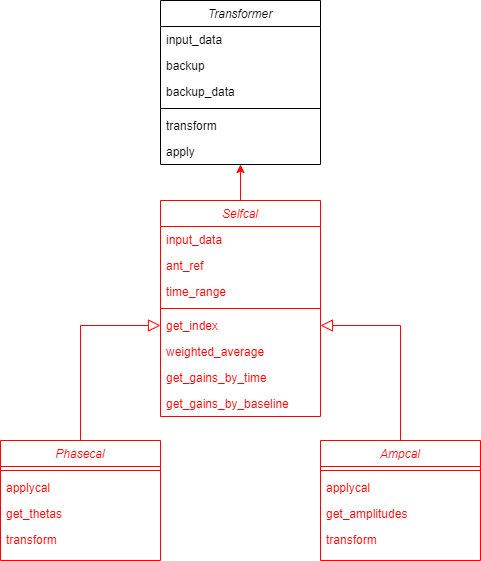
\includegraphics[scale=0.4]{images/Pyralysis-Self-calibration.png}
	\caption[Diagrama de clases Self-calibration]{Diagrama de clases Self-calibration. Fuente: Elaboración propia}
	\label{fig:selfcal_diagram}
\end{figure}

La clase \textit{Selfcal} está constituida por 3 atributos que son \texttt{input\_data} que representa el conjunto de datos, \texttt{ant\_ref} que es la antena de referencia y \texttt{time\_range} que es el rango de tiempo en el cual se quiere calibrar. Está además cuenta con los métodos siguientes: 

\begin{itemize}
    \item \texttt{get\_index}: Método que permite obtener los rangos de tiempos. Este se basa en el algoritmo \ref{alg:get_index}.
    \item \texttt{weighted\_average}: Realiza el promedio ponderado de los ángulos obtenidos.
    \item \texttt{get\_gains\_by\_time}: Realiza el agrupamiento mediante el rango de tiempo y el promedio ponderado para calcular los ángulos obtenidos. 
    \item \texttt{get\_gains\_by\_baseline}: Realiza el promedio ponderado de los ángulos agrupados por \textit{scan\_number}.
\end{itemize}

Las clases \textit{Phasecal} y \textit{Ampcal} tienen algunos métodos nombrados de igual manera pero realizan operaciones distintas. El método \texttt{applycal} permite aplicar los ángulos obtenidos a las visibilidades, donde en \textit{Phasecal} se aplica según la ecuación \ref{eq:applycal} y para \textit{Ampcal} se utiliza la ecuación \ref{eq:amp2}. Por otro lado, el método \texttt{get\_thetas} y \texttt{get\_amplitudes} aplican las ecuaciones \ref{eq:phase5} y \ref{eq:amp1} para así obtener los ángulos y las amplitudes respectivamente. 


\section{Bispectrum}

El método de \textit{Bispectrum} es creado en una clase del mismo nombre, la cual hereda de la clase \textit{Transformer} debido a que el objetivo de la clase \textit{Bispectrum} es realizar un reordenamiento del conjunto de datos ingresado. El diagrama de clases asociado a esta implementación es presentado en la Figura \ref{fig:bispectrum_diagram}.

\begin{figure}[!ht]
	\centering
	\captionsetup{justification=centering}
	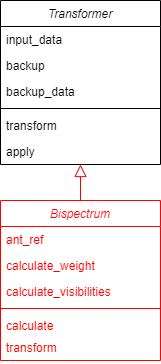
\includegraphics[scale=0.5]{images/Pyralysis-Bispectrum.png}
	\caption[Diagrama de clases para Bispectrum]{Diagrama de clases para Bispectrum. Fuente: Elaboración propia}
	\label{fig:bispectrum_diagram}
\end{figure}

Los atributos de la clase \textit{Bispectrum} son \texttt{ant\_ref} que es un número el cual indica la antena de referencia utilizada para filtrar las combinaciones iniciales, \texttt{calculate\_weight} y \texttt{calculate\_visibilities} son booleanos que indican si se debe calcular o no los pesos y visibilidades observadas en su formato \textit{Bispectrum}. El método \texttt{transform} reorganiza el conjunto de datos de tal manera de tener las visibilidades observadas, modelo y pesos en un arreglo con una dimensión igual a 3, de tal manera que cada dimensión de esta corresponde a una combinación de antenas ($ij$, $jk$ y $ki$). Por otro lado, el método \texttt{calculate} toma el conjunto de datos reordenado por \texttt{transform} y realiza la multiplicación de los datos para las combinaciones de antenas, sin embargo, para el calculo de los pesos se utiliza una variante de la ecuación \ref{eq:sigma} que esta dada por la ecuación \ref{eq:weight_bis} y para su obtención se debe tener en cuenta la ecuación \ref{eq:weights}.

\begin{equation}
    \label{eq:weights}
    w = \frac{1}{\sigma^2}
\end{equation}

\begin{equation}
    \label{eq:weight_bis}
    w_{bis} = \bigg( |V_{B}|^{2} \bigg[ \frac{1}{|V_{1}|^{2} w_{1}} + \frac{1}{|V_{2}|^{2} w_{2}} + \frac{1}{|V_{3}|^{2} w_{3}}\bigg] \bigg)^{-1}
\end{equation}

Para obtener una imagen con los datos obtenidos mediante la clase anterior es necesario definir la función y el gradiente para el \textit{Bispectrum} las cuales deben estar definidas en una clase, por lo mismo se tiene la clase \textit{Chi2Bis} que cumple con lo anterior. Esta clase cuenta con dos atributos llamados \texttt{model\_bispectrum} que es un tipo de objeto que se detallará mas adelante y \texttt{dataset} que es el conjunto de datos ingresado, además de contar con el método \texttt{function} que retorna el valor de la función objetivo definida en la ecuación \ref{eq:bispectrum_2} y el método \texttt{gradient} que retorna el valor del gradiente de la función objetivo y está definida por la ecuación \ref{eq:derivadaBis}.

\begin{figure}[!ht]
	\centering
	\captionsetup{justification=centering}
	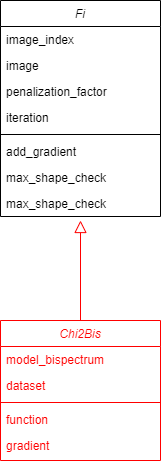
\includegraphics[scale=0.4]{images/Pyralysis-Bispectrum_Chi.png}
	\caption[Diagrama de clases para $\chi^2$ Bispectrum]{Diagrama de clases para $\chi^2$ Bispectrum. Fuente: Elaboración propia}
	\label{fig:bispectrumChi_diagram}
\end{figure}

Como se menciona anteriormente, la clase \textit{Chi2Bis} contiene un objeto llamado \texttt{model\_bispectrum} que viene de la clase del mismo nombre \textit{ModelBispectrum}. Este tiene el objetivo de calcular las visibilidades modelo \textit{Bispectrum} que posteriormente serán utilizadas en el cálculo de la función objetivo y su gradiente. En este \texttt{model\_bispectrum} es un método que permite el cálculo de las visibilidades modelo y su formato \textit{Bispectrum}. 

En el caso del optimizador para resolver la clase \textit{Chi2Bis} está dado por la clase \textit{NonLinearGradient} que hereda de la clase \textit{Optimizer}. Esta clase contiene 5 atributos que son \texttt{line\_search} que es el método de búsqueda lineal a utilizar para el paso del gradiente, \texttt{image} es la imagen inicial para el gradiente ($x_{0}$), \texttt{epsilon} es un número para evitar la división por cero, \textit{error} es el valor aceptable mínimo para el criterio de parada y \texttt{max\_iter} es la cantidad de iteraciones que realiza el gradiente. Para los métodos se tiene \texttt{run} que realiza la ejecución del gradiente conjugado y \texttt{polak\_rebiere} que aplica el método de Polak-Ribiere-Polyak para el calculo de $\beta$.

\begin{figure}[!ht]
	\centering
	\captionsetup{justification=centering}
	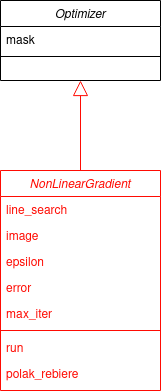
\includegraphics[scale=0.4]{images/Gradient.png}
	\caption[Diagrama de clases para Gradiente Conjugado]{Diagrama de clases para Gradiente Conjugado. Fuente: Elaboración propia}
	\label{fig:pyralysis_gradient}
\end{figure}

Un punto importante a destacar es que para la implementación de esta clase se utiliza el patrón de diseño \textit{Decorator} mencionado en la sección \ref{subsec:patrones}. Este se utiliza debido a la ventaja que trae al poder utilizar el método \texttt{transform} de la clase \textit{ModelVisibilities} y a la vez definir un método \texttt{transform} en \textit{ModelBispectrum} de manera que no se tenga que duplicar código y permitiendo respetar que el método \texttt{transform} en la clase \textit{Transformer} se define como un método abstracto, por lo que debe estar presente en todas sus clases hijas. 

\begin{figure}[!ht]
	\centering
	\captionsetup{justification=centering}
	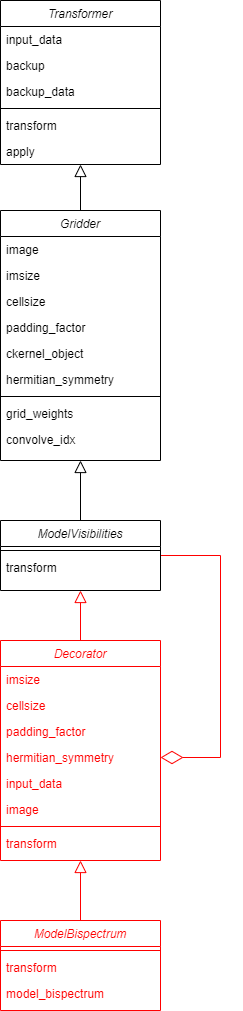
\includegraphics[scale=0.4]{images/Pyralysis-ModelBispectrum.png}
	\caption[Diagrama de clases para ModelBispectrum]{Diagrama de clases para ModelBispectrum. Fuente: Elaboración propia}
	\label{fig:modelBispectrum_diagram}
\end{figure}

Finalmente, para es necesaria la creación de una clase capaz de guardar los nuevos datos creados con \textit{Bispectrum}. La clase \textit{VisibilityBis} cumple con este objetivo al tener atributos que permiten el almacenamiento de las visibilidades y otros datos en su formato \textit{Bispectrum}, además esta clase hereda de la clase ya implementada en Pyralysis llamada \textit{VisibilitySet}, como se muestra en la Figura \ref{fig:visibilityBis_diagram}, de tal manera que se puede acceder a todos los atributos del conjunto de datos original. Los atributos que tiene la clase \textit{VisibilityBis} son los siguientes:

\begin{itemize}
    \item \texttt{antenna3}: Antena $k$ para combinación de antenas $i,j,k$.
    \item \texttt{bis\_data} y \texttt{bis\_model}: Visbilidades observadas y modelo respectivamente en su formato \textit{Bispectrum}.
    \item \texttt{bis\_uvw}: Datos UVW del conjunto de datos original ordenados en su formato \textit{Bispectrum}.
    \item \texttt{bis\_weight}: Pesos del conjunto de datos original ordenados en su formato \textit{Bispectrum}.
    \item \texttt{bis\_ant\_ref}: Antena de referencia utilizado para realizar el \textit{Bispectrum}.
\end{itemize}

\begin{figure}[!ht]
	\centering
	\captionsetup{justification=centering}
	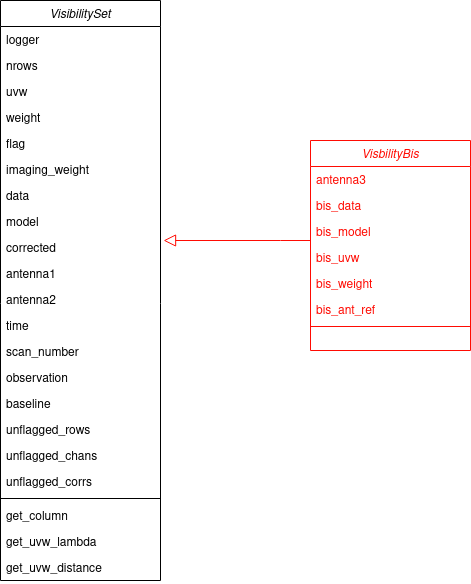
\includegraphics[scale=0.4]{images/Pyralysis-Visibility_bis.png}
	\caption[Diagrama de clases para VisibilityBis]{Diagrama de clases para VisibilityBis. Fuente: Elaboración propia}
	\label{fig:visibilityBis_diagram}
\end{figure}

\chapter{Resultados}
\label{cap:resultados}

A continuación se presentan los resultados obtenidos con los métodos creados junto a sus métricas asociadas, así como también se presentan las comparaciones relacionadas a otros métodos tanto para los conjuntos de datos simulados como los reales. 

\section{Datos simulados}

\subsection{Self-calibration}

\subsubsection{\textit{Long-baseline}}

La prueba de \textit{self-calibration} utiliza el conjunto de datos simulado creado en la sección \ref{sec:simulated_data}, sin embargo estas vienen perturbadas por una ganancia aleatoria que está asignada a una antena, donde la imagen resultante de esta puede ser vista en la Figura \ref{fig:noisy_image}. Cabe destacar que los datos perturbados son aquellos asociados a una antena de referencia, que para el caso del conjunto de datos reducidos de HD163296 sería la antena DA48, así como también se considera todos los parámetros proporcionados por los scripts que se pueden encontrar en el sitio web de DSHARP, específicamente el asociado al conjunto de datos HD163296. 

\begin{figure}[!ht]
 \centering
  \subfloat[Original]{
   \label{fig:noisy_original}
    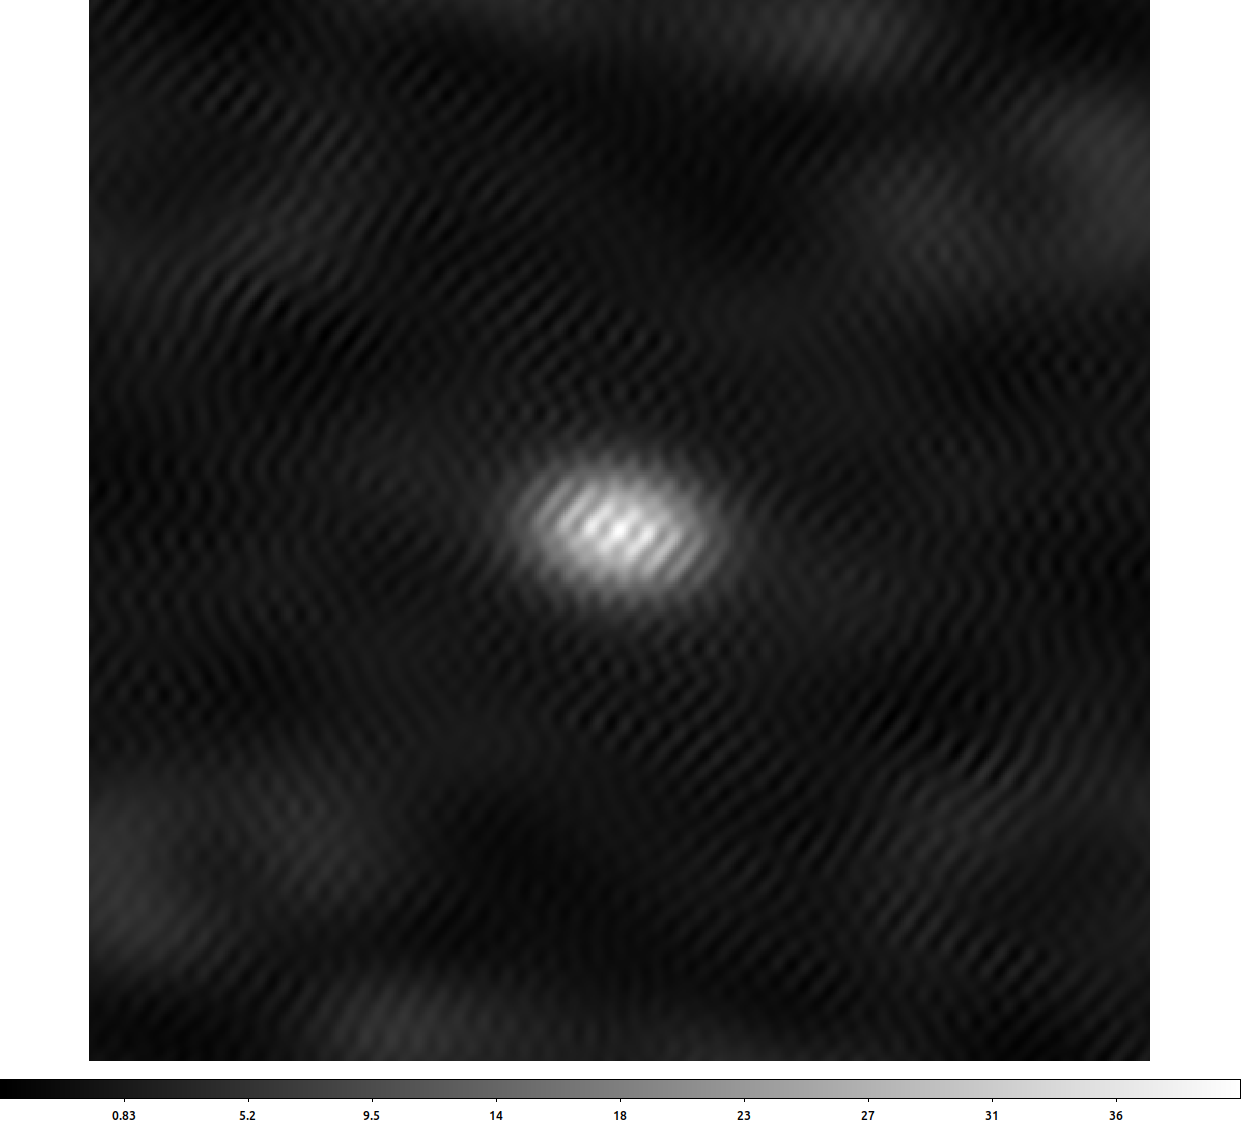
\includegraphics[width=0.45\textwidth]{images/noisy_dataset_dirty.png}}
  \subfloat[Color]{
   \label{fig:noisy_color}
    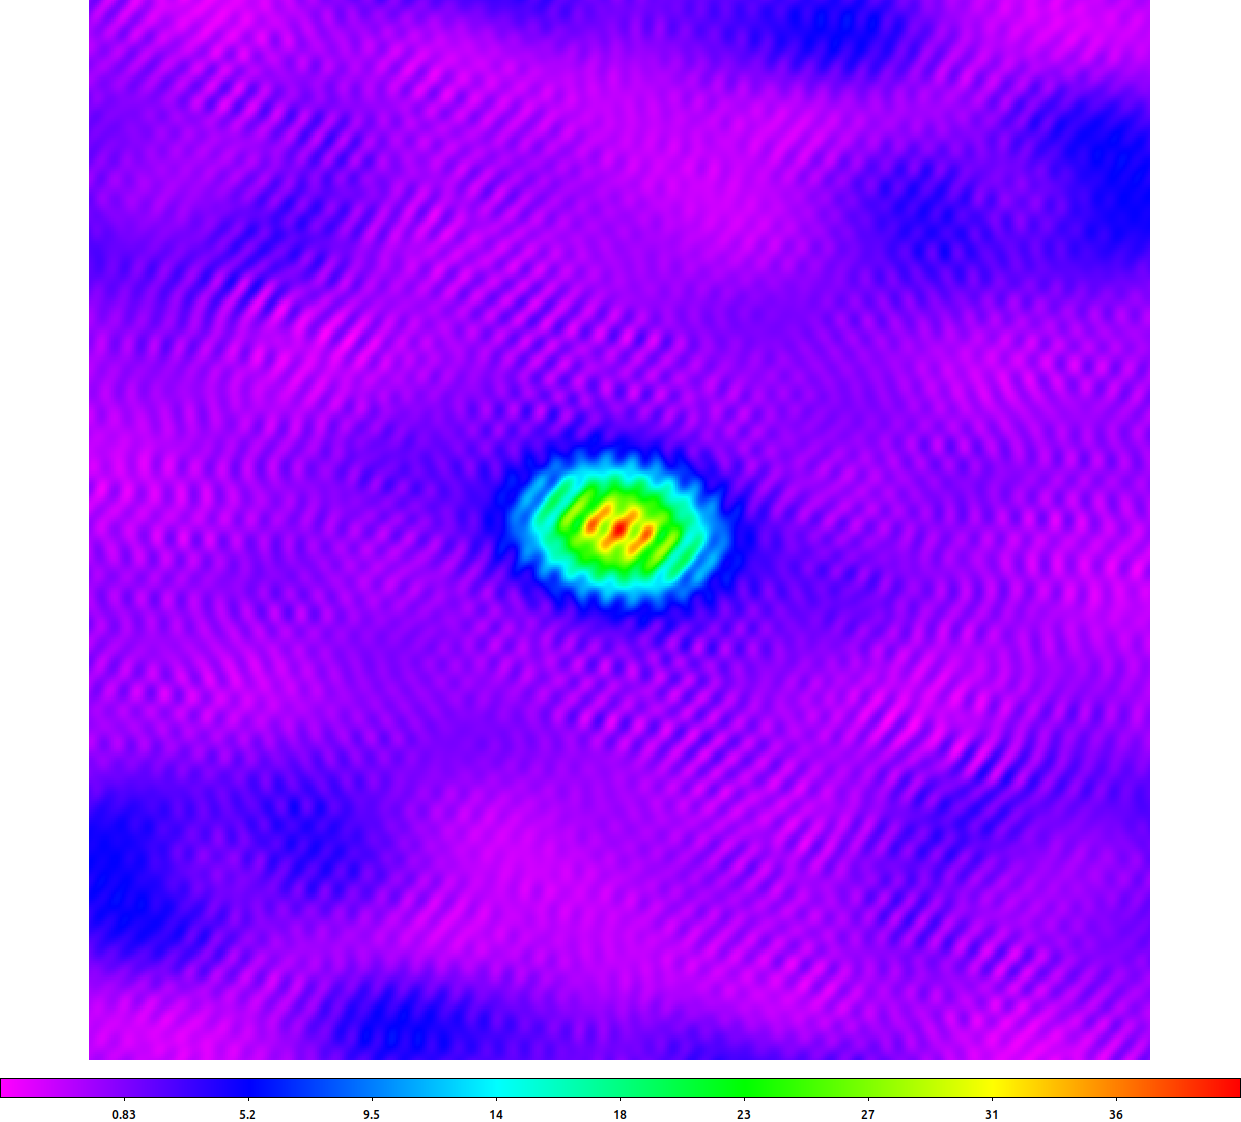
\includegraphics[width=0.45\textwidth]{images/noisy_dataset_dirty_color.png}}
 \caption[Imagen simulado afectada por una fase (\textit{long-baseline})]{Imagen simulado afectada por una fase (\textit{long-baseline}). Fuente: Elaboración propia.}
 \label{fig:noisy_image}
\end{figure}

La síntesis de imágenes es realizada a través de los algoritmos de CLEAN y MEM a través de las herramientas CASA y GPUVMEM. En este momento no se considera la ejecución del algoritmo \textit{Bispectrum} debido a que en esta sección se desea mostrar la eficacia del algoritmo para \textit{self-calibration} desarrollado. 

Para la primera iteración se realiza una calibración de fase considerando un rango de tiempo de 360 segundos. En la figura \ref{fig:phasecal_1iter} se observa el resultado obtenido luego de realizar el método CLEAN al conjunto de datos calibrado donde este obtuvo un valor de PSNR de 218.1818 y un NRMSE de 0.986209. Por otro lado, en la Figura \ref{fig:phasecal_1iter_gpuvmem} se observa el resultado luego de realizar el método MEM sobre el conjunto de datos calibrado, obteniendo así un PSNR de 219.3238 y un NRMSE 0.705504.

\begin{figure}[!ht]
 \centering
  \subfloat[Original]{
   \label{fig:clean_original_clean_1iter}
    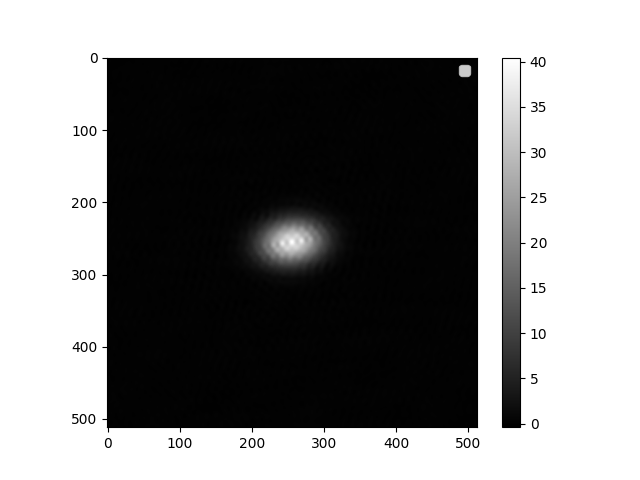
\includegraphics[width=0.5\textwidth]{images/sim_p0_long.png}}
  \subfloat[Color]{
   \label{fig:clean_original_color_1iter}
    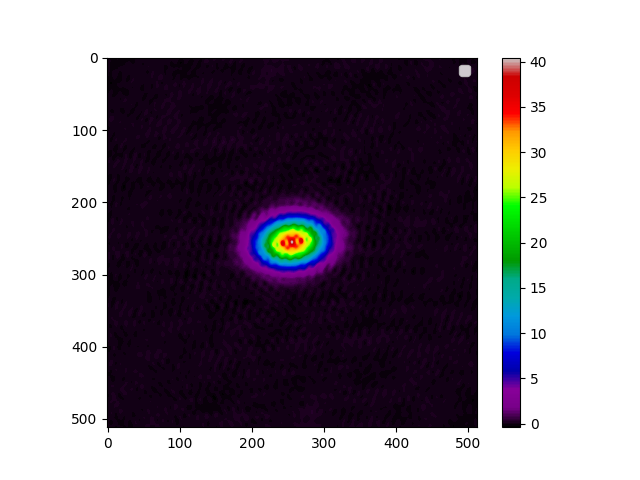
\includegraphics[width=0.5\textwidth]{images/sim_p0_long_color.png}}
    \vspace{0.3cm}
  \subfloat[Residuos Original]{
   \label{fig:clean_residual_clean_1iter}
    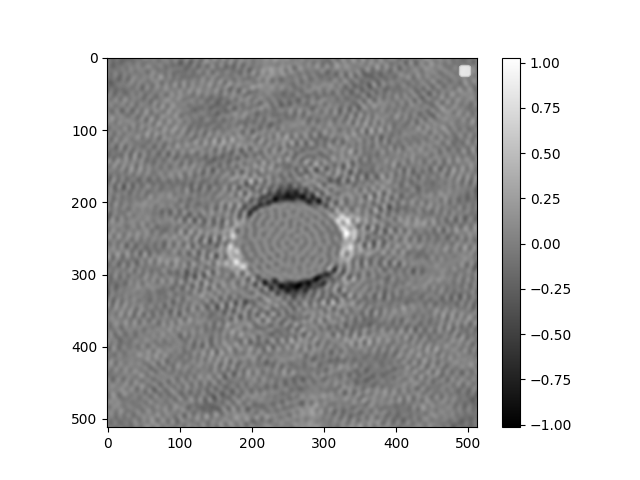
\includegraphics[width=0.5\textwidth]{images/sim_p0_long_residual.png}}
  \subfloat[Residuos Color]{
   \label{fig:clean_resisdual_color_1iter}
    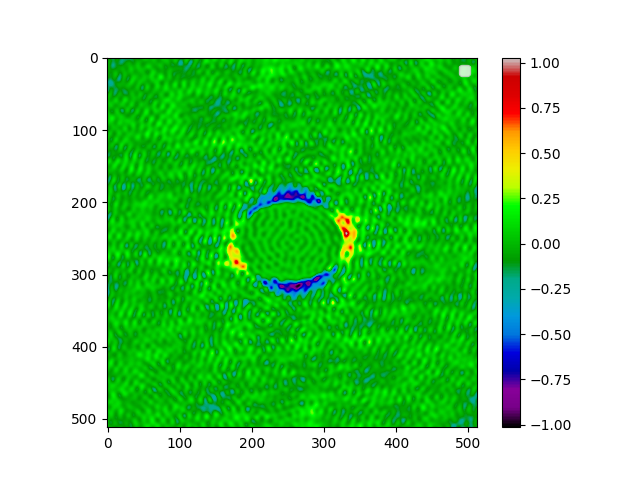
\includegraphics[width=0.5\textwidth]{images/sim_p0_long_color_residual.png}}
 \caption[Primera iteración para conjunto de datos simulado CLEAN (\textit{long-baseline})]{Primera iteración para conjunto de datos simulado CLEAN (\textit{long-baseline}). Fuente: Elaboración propia.}
 \label{fig:phasecal_1iter}
\end{figure}

\begin{figure}[!ht]
 \centering
  \subfloat[Original]{
   \label{fig:gpuvmem_original_1iter}
    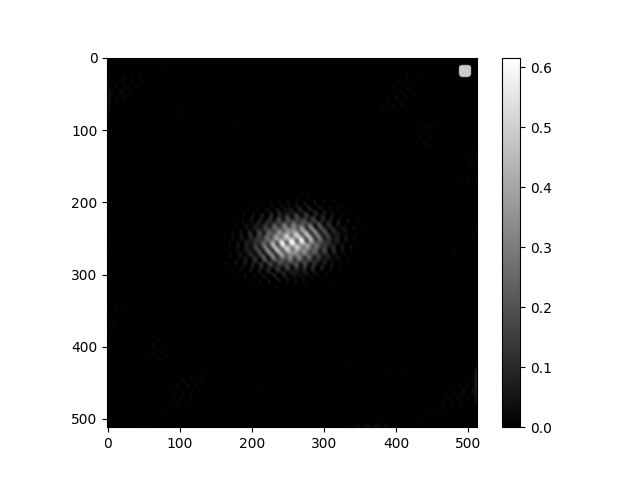
\includegraphics[width=0.5\textwidth]{images/sim_p0_long_gpuvmem.png}}
  \subfloat[Color]{
   \label{fig:gpuvmem_color_1iter}
    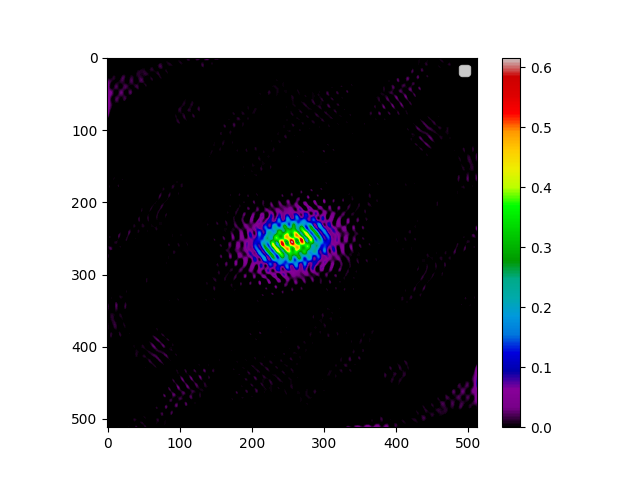
\includegraphics[width=0.5\textwidth]{images/sim_p0_long_gpuvmem_color.png}}
    \vspace{0.3cm}
  \subfloat[Original]{ 
   \label{fig:gpuvmem_residual_original_1iter}
    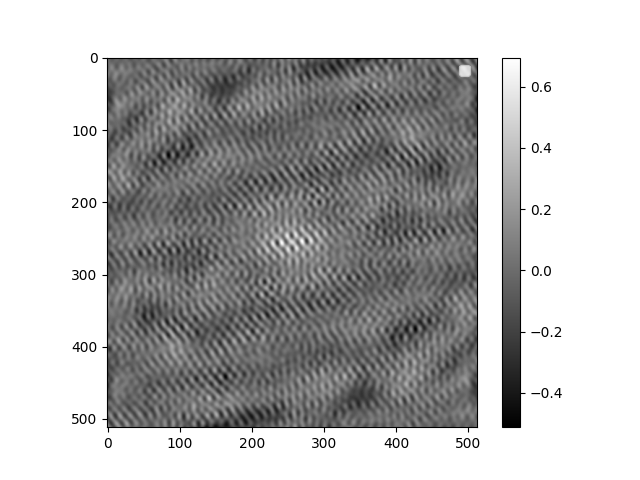
\includegraphics[width=0.5\textwidth]{images/sim_p0_long_gpuvmem_residual.png}}
  \subfloat[Color]{
   \label{fig:gpuvmem_residual_color_1iter}
    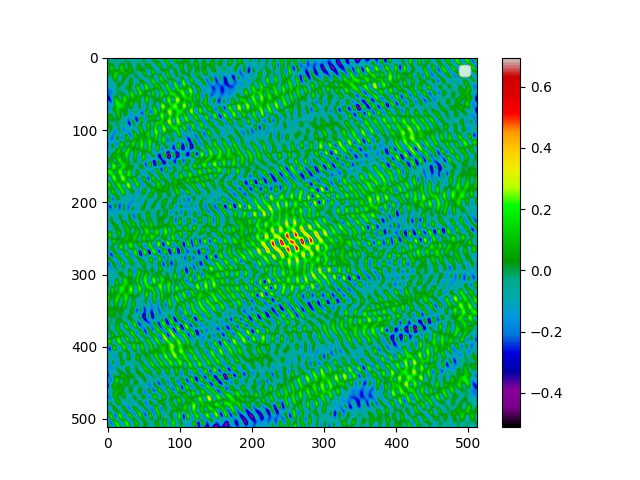
\includegraphics[width=0.5\textwidth]{images/sim_p0_long_gpuvmem_color_residual.png}}
 \caption[Primera iteración para conjunto de datos simulado GPUVMEM (\textit{long-baseline})]{Primera iteración para conjunto de datos simulado GPUVMEM (\textit{long-baseline}). Fuente: Elaboración propia.}
 \label{fig:phasecal_1iter_gpuvmem}
\end{figure}

Una segunda iteración de fase se realiza con un rango de tiempo de 120 segundos considerando la misma antena de referencia. En la Figura \ref{fig:phasecal_2iter} se puede ver el resultado obtenido con el método CLEAN al aplicarse en el conjunto nuevamente calibrado, donde este obtuvo un PSNR de 224.1047 y un NRMSE de 0.986204, en cambio, la Figura \ref{fig:phasecal_2iter_gpuvmem} muestra el resultado con el método MEM donde este obtuvo un PSNR de 218.4566 y un NRMSE de 0.706291. 

\begin{figure}[!ht]
 \centering
  \subfloat[Original]{
   \label{fig:clean_original_clean_2iter}
    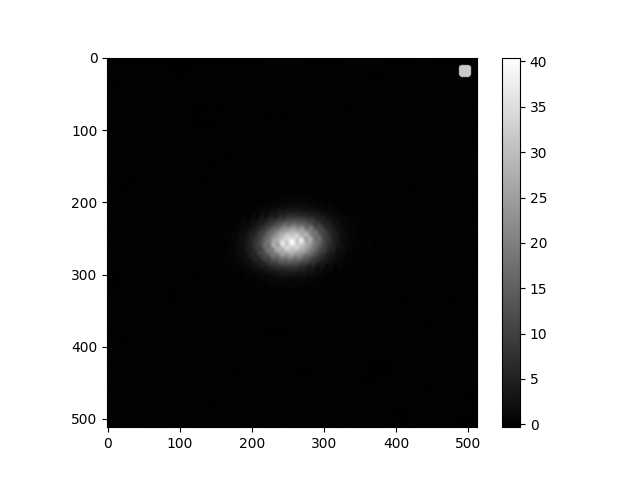
\includegraphics[width=0.5\textwidth]{images/sim_p1_long.png}}
  \subfloat[Color]{
   \label{fig:clean_original_color_2iter}
    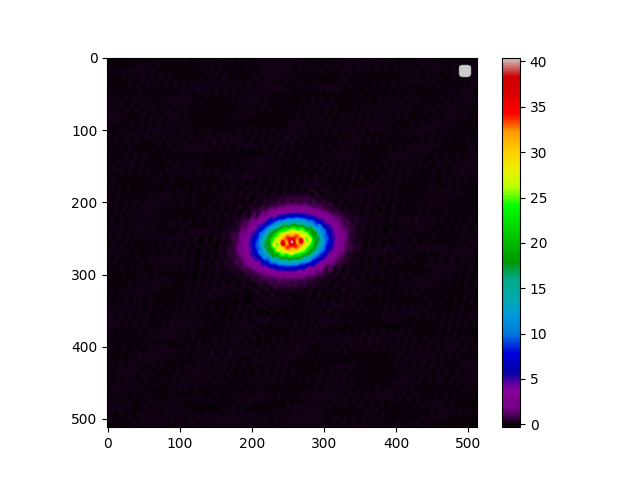
\includegraphics[width=0.5\textwidth]{images/sim_p1_long_color.png}}
    \vspace{0.3cm}
  \subfloat[Residuos Original]{
   \label{fig:clean_residual_clean_2iter}
    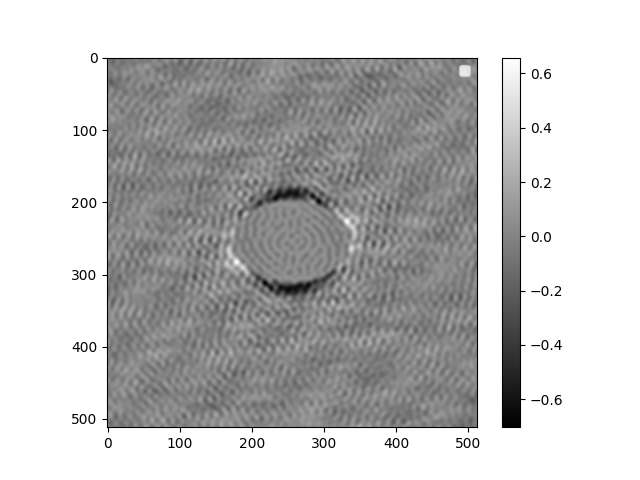
\includegraphics[width=0.5\textwidth]{images/sim_p1_long_residual.png}}
  \subfloat[Residuos Color]{
   \label{fig:clean_residual_color_2iter}
    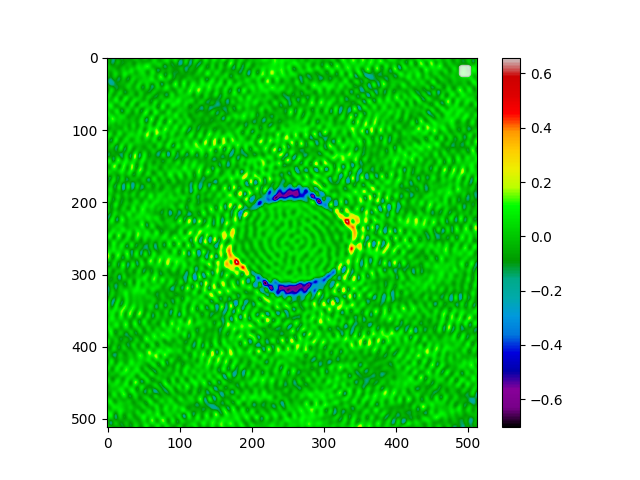
\includegraphics[width=0.5\textwidth]{images/sim_p1_long_color_residual.png}}
 \caption[Segunda iteración para conjunto de datos simulado CLEAN (\textit{long-baseline})]{Segunda iteración para conjunto de datos simulado CLEAN (\textit{long-baseline}). Fuente: Elaboración propia.}
 \label{fig:phasecal_2iter}
\end{figure}

\begin{figure}[!ht]
 \centering
  \subfloat[Original]{
   \label{fig:gpuvmem_original_2iter}
    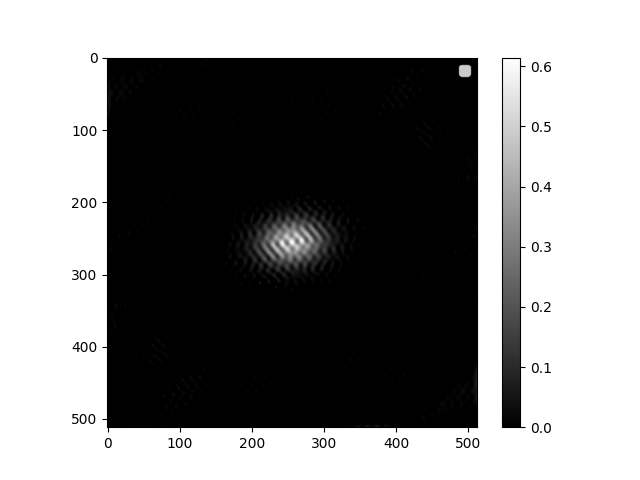
\includegraphics[width=0.5\textwidth]{images/sim_p1_long_gpuvmem.png}}
  \subfloat[Color]{
   \label{fig:gpuvmem_color_2iter}
    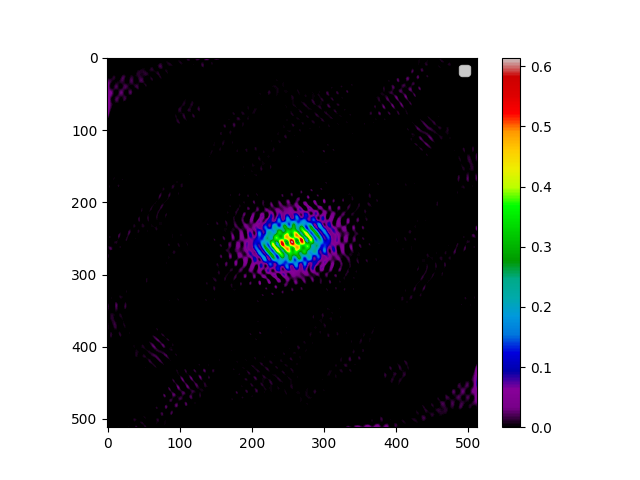
\includegraphics[width=0.5\textwidth]{images/sim_p1_long_gpuvmem_color.png}}
    \vspace{0.3cm}
    \subfloat[Residuo Original]{
   \label{fig:gpuvmem_original_2iter_residual}
    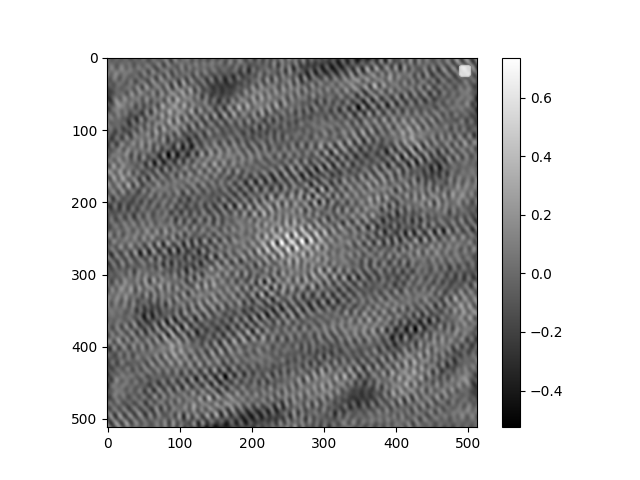
\includegraphics[width=0.5\textwidth]{images/sim_p1_long_gpuvmem_residual.png}}
  \subfloat[Residuo Color]{
   \label{fig:gpuvmem_color_2iter_residual}
    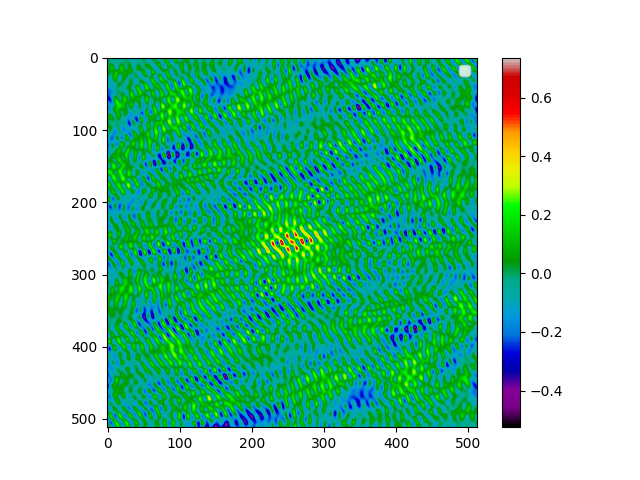
\includegraphics[width=0.5\textwidth]{images/sim_p1_long_gpuvmem_color_residual.png}}
 \caption[Segunda iteración para conjunto de datos simulado GPUVMEM (\textit{long-baseline})]{Segunda iteración para conjunto de datos simulado GPUVMEM (\textit{long-baseline}). Fuente: Elaboración propia.}
 \label{fig:phasecal_2iter_gpuvmem}
\end{figure}

La tercera iteración se realiza el \textit{self-calibration} de fase, considerando un tiempo de 60 segundos con la misma antena de referencia que las antenas anteriores. La Figura \ref{fig:phasecal_3iter} y la Figura \ref{fig:phasecal_3iter_gpuvmem} muestran los valores obtenidos con los métodos de CLEAN y MEM respectivamente, donde la primera obtuvo un PSNR de 217.3753 y un NRMSE de 0.985206, en cambio la otra obtuvo un PSNR de 218.0049  y un NRMSE de 0.706730.  

\begin{figure}[!ht]
 \centering
  \subfloat[Original]{
   \label{fig:clean_original_clean_3iter}
    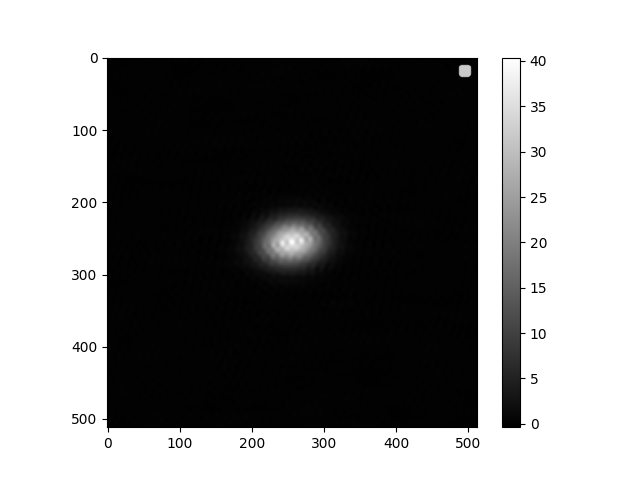
\includegraphics[width=0.5\textwidth]{images/sim_p2_long.png}}
  \subfloat[Color]{
   \label{fig:clean_original_color_3iter}
    \includegraphics[width=0.5\textwidth]{images/sim_p2_long_color.png}}
    \vspace{0.3cm}
  \subfloat[Residuos Original]{
   \label{fig:clean_residual_clean_3iter}
    \includegraphics[width=0.5\textwidth]{images/sim_p2_long_residual.png}}
  \subfloat[Residuos Color]{
   \label{fig:clean_residual_color_3iter}
    \includegraphics[width=0.5\textwidth]{images/sim_p2_long_color_residual.png}}
 \caption[Tercera iteración para conjunto de datos simulado CLEAN (\textit{long-baseline})]{Tercera iteración para conjunto de datos simulado CLEAN (\textit{long-baseline}). Fuente: Elaboración propia.}
 \label{fig:phasecal_3iter}
\end{figure}

\begin{figure}[!ht]
 \centering
  \subfloat[Original]{
   \label{fig:gpuvmem_original_3iter}
    \includegraphics[width=0.5\textwidth]{images/sim_p2_long_gpuvmem.png}}
  \subfloat[Color]{
   \label{fig:gpuvmem_color_3iter}
    \includegraphics[width=0.5\textwidth]{images/sim_p2_long_gpuvmem_color.png}}
    \vspace{0.3cm}
  \subfloat[Residuos Original]{
   \label{fig:gpuvmem_original_3iter_residual}
    \includegraphics[width=0.5\textwidth]{images/sim_p2_long_gpuvmem_residual.png}}
  \subfloat[Residuos Color]{
   \label{fig:gpuvmem_color_3iter_residual}
    \includegraphics[width=0.5\textwidth]{images/sim_p2_long_gpuvmem_color_residual.png}}
 \caption[Tercera iteración para conjunto de datos simulado GPUVMEM (\textit{long-baseline})]{Tercera iteración para conjunto de datos simulado GPUVMEM (\textit{long-baseline}). Fuente: Elaboración propia.}
 \label{fig:phasecal_3iter_gpuvmem}
\end{figure}

Una cuarta iteración de calibración de fase se realiza considerando un rango de tiempo de 30 segundos, manteniendo la antena de referencia. La Figura \ref{fig:phasecal_4iter} muestra las imágenes reconstruidas y sus residuos mediante el método CLEAN, por otro lado en la Figura \ref{fig:phasecal_4iter_gpuvmem} se ve las imágenes reconstruidas y su residuo. Los valores PSNR para la primera imagen es de 222.6623 y su NRMSE es 0.986208, mientras que para la segunda su PSNR es 220.1864 y su NRMSE 0.763954. 


\begin{figure}[!ht]
 \centering
  \subfloat[Original]{
   \label{fig:clean_original_clean_4iter}
    \includegraphics[width=0.5\textwidth]{images/sim_p3_long.png}}
  \subfloat[Color]{
   \label{fig:clean_original_color_4iter}
    \includegraphics[width=0.5\textwidth]{images/sim_p3_long_color.png}}
    \vspace{0.3cm}
  \subfloat[Residuos Original]{
   \label{fig:clean_residual_clean_4iter}
    \includegraphics[width=0.5\textwidth]{images/sim_p3_long_residual.png}}
  \subfloat[Residuos Color]{
   \label{fig:clean_residual_color_4iter}
    \includegraphics[width=0.5\textwidth]{images/sim_p3_long_color_residual.png}}
 \caption[Cuarta iteración para conjunto de datos simulado CLEAN (\textit{long-baseline})]{Cuarta iteración para conjunto de datos simulado CLEAN (\textit{long-baseline}). Fuente: Elaboración propia.}
 \label{fig:phasecal_4iter}
\end{figure}

\begin{figure}[!ht]
 \centering
  \subfloat[Original]{
   \label{fig:gpuvmem_original_4iter}
    \includegraphics[width=0.5\textwidth]{images/sim_p3_long_gpuvmem.png}}
  \subfloat[Color]{
   \label{fig:gpuvmem_color_4iter}
    \includegraphics[width=0.5\textwidth]{images/sim_p3_long_gpuvmem_color.png}}
    \vspace{0.3cm}
  \subfloat[Residuos Original]{
   \label{fig:gpuvmem_original_4iter_residual}
    \includegraphics[width=0.5\textwidth]{images/sim_p3_long_gpuvmem_residual.png}}
  \subfloat[Residuos Color]{
   \label{fig:gpuvmem_color_4iter_residual}
    \includegraphics[width=0.5\textwidth]{images/sim_p3_long_gpuvmem_color_residual.png}}
 \caption[Cuarta iteración para conjunto de datos simulado GPUVMEM (\textit{long-baseline})]{Cuarta iteración para conjunto de datos simulado GPUVMEM (\textit{long-baseline}). Fuente: Elaboración propia.}
 \label{fig:phasecal_4iter_gpuvmem}
\end{figure}

La quinta iteración también considera una calibración de fase pero con un rango de tiempo de 18 segundos, donde se sigue manteniendo la antena de referencia. En la Figura \ref{fig:phasecal_5iter} se observa los resultados obtenidos con el método CLEAN donde su PSNR tiene un valor de 219.3188 y su NRMSE de 0.986208. Por otro lado la Figura \ref{fig:phasecal_5iter_gpuvmem} se observa el resultado obtenido con MEM, donde su PSNR tiene un valor de 225.1549  y su NRMSE es de 0.706844.

\begin{figure}[!ht]
 \centering
  \subfloat[Original]{
   \label{fig:clean_original_clean_5iter}
    \includegraphics[width=0.5\textwidth]{images/sim_p4_long.png}}
  \subfloat[Color]{
   \label{fig:clean_original_color_5iter}
    \includegraphics[width=0.5\textwidth]{images/sim_p4_long_color.png}}
    \vspace{0.3cm}
  \subfloat[Residuos Original]{
   \label{fig:clean_residual_clean_5iter}
    \includegraphics[width=0.5\textwidth]{images/sim_p4_long_residual.png}}
  \subfloat[Residuos Color]{
   \label{fig:clean_residual_color_5iter}
    \includegraphics[width=0.5\textwidth]{images/sim_p4_long_color_residual.png}}
 \caption[Quinta iteración para conjunto de datos simulado CLEAN (\textit{long-baseline})]{Quinta iteración para conjunto de datos simulado CLEAN (\textit{long-baseline}). Fuente: Elaboración propia.}
 \label{fig:phasecal_5iter}
\end{figure}

\begin{figure}[!ht]
 \centering
  \subfloat[Original]{
   \label{fig:gpuvmem_original_5iter}
    \includegraphics[width=0.5\textwidth]{images/sim_p4_long_gpuvmem.png}}
  \subfloat[Color]{
   \label{fig:gpuvmem_color_5iter}
    \includegraphics[width=0.5\textwidth]{images/sim_p4_long_gpuvmem_color.png}}
    \vspace{0.3cm}
  \subfloat[Residuos Original]{
   \label{fig:gpuvmem_original_5iter_residual}
    \includegraphics[width=0.5\textwidth]{images/sim_p4_long_gpuvmem_residual.png}}
  \subfloat[Residuos Color]{
   \label{fig:gpuvmem_color_5iter_residual}
    \includegraphics[width=0.5\textwidth]{images/sim_p4_long_color_residual.png}}
 \caption[Quinta iteración para conjunto de datos simulado GPUVMEM (\textit{long-baseline})]{Quinta iteración para conjunto de datos simulado GPUVMEM (\textit{long-baseline}). Fuente: Elaboración propia.}
 \label{fig:phasecal_5iter_gpuvmem}
\end{figure}

Una sexta y última iteración se realiza pero esta vez tanto en amplitud y fase, considerando un tiempo designado como \texttt{inf}, que quiere decir que se realiza por \textit{scan\_number}. La imagen reconstruida con CLEAN se puede ver en la Figura \ref{fig:phasecal_6ter} que tiene un PSNR de 217.0193 y un NRMSE de 0.986210, por otro lado la imagen reconstruida con MEM se puede observar en la Figura \ref{fig:phasecal_6iter_gpuvmem} done esta tiene un PSNR de 219.5513 y un NRMSE de 0.705273. 

\begin{figure}[!ht]
 \centering
  \subfloat[Original]{
   \label{fig:clean_original_clean_6iter}
    \includegraphics[width=0.5\textwidth]{images/sim_p5_long.png}}
  \subfloat[Color]{
   \label{fig:clean_original_color_6iter}
    \includegraphics[width=0.5\textwidth]{images/sim_p5_long_color.png}}
    \vspace{0.3cm}
  \subfloat[Residuos Original]{
   \label{fig:clean_residual_clean_6iter}
    \includegraphics[width=0.5\textwidth]{images/sim_p5_long_residual.png}}
  \subfloat[Residuos Color]{
   \label{fig:clean_residual_color_6iter}
    \includegraphics[width=0.5\textwidth]{images/sim_p5_long_color_residual.png}}
 \caption[Sexta iteración para conjunto de datos simulado CLEAN (\textit{long-baseline})]{Sexta iteración para conjunto de datos simulado CLEAN (\textit{long-baseline}). Fuente: Elaboración propia.}
 \label{fig:phasecal_6ter}
\end{figure}

\begin{figure}[!ht]
 \centering
  \subfloat[Original]{
   \label{fig:gpuvmem_original_6iter}
    \includegraphics[width=0.5\textwidth]{images/sim_p5_long_gpuvmem.png}}
  \subfloat[Color]{ 
   \label{fig:gpuvmem_color_6iter}
    \includegraphics[width=0.5\textwidth]{images/sim_p5_long_gpuvmem_color.png}}
    \vspace{0.3cm}
  \subfloat[Residuos Original]{
   \label{fig:gpuvmem_original_6iter_residual}
    \includegraphics[width=0.5\textwidth]{images/sim_p5_long_gpuvmem_residual.png}}
  \subfloat[Residuos Color]{
   \label{fig:gpuvmem_color_6iter_residual}
    \includegraphics[width=0.5\textwidth]{images/sim_p5_long_color_residual.png}}
 \caption[Sexta iteración para conjunto de datos simulado GPUVMEM (\textit{long-baseline})]{Sexta iteración para conjunto de datos simulado GPUVMEM (\textit{long-baseline}). Fuente: Elaboración propia.}
 \label{fig:phasecal_6iter_gpuvmem}
\end{figure}


En la tabla \ref{tab:sim_long_selfcal_psnr} se puede observar un resumen de los valores para el PSNR de las iteraciones mostradas anteriormente, mientras que en la tabla \ref{tab:sim_long_selfcal_nrmse} se puede observar una tabla resumen con los valores de NRMSE obtenidos para las distintas iteraciones. 

\begin{table}[!ht]
	\begin{center}
		\caption{Tabla con PSNR para \textit{self-calibration} de datos simulados \textit{long-baseline}.}
		\begin{tabular}{| c | c | c |}
			\hline
			Iteración & CLEAN & MEM\\ \hline
			Primera & 218.1818 & 219.3238\\ \hline
            Segunda & 224.1047 & 218.4566\\ \hline
            Tercera & 217.3753 & 218.0049\\ \hline
            Cuarta & 222.6623 & 220.1864\\ \hline
            Quinta & 219.3188 & 225.1549\\ \hline
            Sexta & 217.0193 & 219.5513\\ \hline
		\end{tabular}
		\label{tab:sim_long_selfcal_psnr}
	\end{center}
	\begin{center}
		Fuente: Elaboración propia.
	\end{center}
\end{table}

\begin{table}[!ht]
	\begin{center}
		\caption{Tabla con NRMSE para \textit{self-calibration} de datos simulados \textit{long-baseline}.}
		\begin{tabular}{| c | c | c |}
			\hline
			Iteración & CLEAN & MEM\\ \hline
			Primera & 0.986209 & 0.705504\\ \hline
            Segunda & 0.986204 & 0.706291\\ \hline
            Tercera & 0.986206 & 0.706730\\ \hline
            Cuarta & 0.986203 & 0.763954\\ \hline
            Quinta & 0.986208 & 0.706844\\ \hline
            Sexta & 0.986210 & 0.705273\\ \hline
		\end{tabular}
		\label{tab:sim_long_selfcal_nrmse}
	\end{center}
	\begin{center}
		Fuente: Elaboración propia.
	\end{center}
\end{table}

\subsubsection{\textit{Short-baseline}}

Al igual que en el caso anterior las visibilidades asociado al conjunto de datos vienen perturbadas por una ganancia aleatoria, donde existe una ganancia para cada antena. De esta manera también se escoge una antena de referencia para perturbar solamente las visibilidades asociadas a está antena, para el cual en este caso la antena seleccionada es la DA63. La imagen de este conjunto de datos perturbado puede ser vista en la Figura \ref{fig:dirty_short_baseline}. 

\begin{figure}[!ht]
 \centering
  \subfloat[Original]{
   \label{fig:dirty_original_short}
    \includegraphics[width=0.5\textwidth]{images/noisy_14ant.png}}
  \subfloat[Color]{
   \label{fig:color_original_short}
    \includegraphics[width=0.5\textwidth]{images/noisy_14ant_color.png}}
 \caption[Imagen simulada afectada por una fase (\textit{short-baseline})]{Imagen simulada afectada por una fase (\textit{short-baseline}) Fuente: Elaboración propia.}
 \label{fig:dirty_short_baseline}
\end{figure}

La primera iteración se realiza el método de \textit{self-calibration} en la fase, en la cual se considera una duración de 0 segundos para el rango de tiempo. La Figura \ref{fig:short_sim_p0} muestra la imagen resultante del método CLEAN y la Figura \ref{fig:short_sim_p0_gpuvmem} muestra el resultado mediante el método de MEM, con sus residuos respectivos. Para la imagen con CLEAN se obtuvo un PSNR de 28.7411 y un NRMSE de 0.988454, en cambio para la obtenida con MEM se obtuvo un PSNR de 53.9672 y un NRMSE de 1.012773. 

\begin{figure}[!ht]
 \centering
  \subfloat[Original]{
   \label{fig:short_p0_original}
    \includegraphics[width=0.5\textwidth]{images/short_p0_original.png}}
  \subfloat[Color]{
   \label{fig:short_p0_color}
    \includegraphics[width=0.5\textwidth]{images/short_p0_color.png}}
\vspace{0.3cm}
    \subfloat[Residuos Original]{
   \label{fig:short_p0_original_residual}
    \includegraphics[width=0.5\textwidth]{images/short_p0_original_residual.png}}
  \subfloat[Residuos Color]{
   \label{fig:short_p0_color_residual}
    \includegraphics[width=0.5\textwidth]{images/short_p0_color_residual.png}}
 \caption[Primera iteración para conjunto de datos simulado CLEAN (\textit{short-baseline})]{Primera iteración para conjunto de datos simulado CLEAN (\textit{short-baseline}) Fuente: Elaboración propia.}
 \label{fig:short_sim_p0}
\end{figure}

\begin{figure}[!ht]
 \centering
  \subfloat[Original]{
   \label{fig:short_p0_original_gpuvmem}
    \includegraphics[width=0.5\textwidth]{images/sim_p0_long_gpuvmem.png}}
  \subfloat[Color]{
   \label{fig:short_p0_color_gpuvmem}
    \includegraphics[width=0.5\textwidth]{images/sim_p0_short_gpuvmem_color.png}}
\vspace{0.3cm}
    \subfloat[Residuos Original]{
   \label{fig:short_p0_original_residual_gpuvmem}
    \includegraphics[width=0.5\textwidth]{images/sim_p0_short_gpuvmem_residual.png}}
  \subfloat[Residuos Color]{
   \label{fig:short_p0_color_residual_gpuvmem}
    \includegraphics[width=0.5\textwidth]{images/sim_p0_short_gpuvmem_residual_color.png}}
 \caption[Primera iteración para conjunto de datos simulado MEM (\textit{short-baseline})]{Primera iteración para conjunto de datos simulado MEM (\textit{short-baseline}) Fuente: Elaboración propia.}
 \label{fig:short_sim_p0_gpuvmem}
\end{figure}

Una segunda iteración es realizada pero esta vez mediante el método de \textit{self-calibration} en la amplitud, considerando una duración de 60 segundos para el rango de tiempo. La imagen resultante mediante el método CLEAN para esta segunda iteración puede ser vista en la Figura \ref{fig:short_sim_p1} donde se obtuvo un PSNR de 28.7418 además de un NRMSE de 0.988429 y mediante el método de MEM puede ser vista en la Figura \ref{fig:short_sim_p1_gpuvmem} donde se obtuvo un PSNRE de 51.1989 y un NRMSE de 1.002735. 

\begin{figure}[!ht]
 \centering
  \subfloat[Original]{
   \label{fig:short_p1_original}
    \includegraphics[width=0.5\textwidth]{images/short_p1_original.png}}
  \subfloat[Color]{
   \label{fig:short_p1_color}
    \includegraphics[width=0.5\textwidth]{images/short_p1_color.png}}
\vspace{0.3cm}
    \subfloat[Residuos Original]{
   \label{fig:short_p1_original_residual}
    \includegraphics[width=0.5\textwidth]{images/short_p1_original_residual.png}}
  \subfloat[Residuos Color]{
   \label{fig:short_p1_color_residual}
    \includegraphics[width=0.5\textwidth]{images/short_p1_color_residual.png}}
 \caption[Segunda iteración para conjunto de datos simulado CLEAN (\textit{short-baseline})]{Segunda iteración para conjunto de datos simulado CLEAN (\textit{short-baseline}) Fuente: Elaboración propia.}
 \label{fig:short_sim_p1}
\end{figure}

\begin{figure}[!ht]
 \centering
  \subfloat[Original]{
   \label{fig:short_p1_original_gpuvmem}
    \includegraphics[width=0.5\textwidth]{images/sim_p1_short_gpuvmem.png}}
  \subfloat[Color]{
   \label{fig:short_p1_color_gpuvmem}
    \includegraphics[width=0.5\textwidth]{images/sim_p1_short_gpuvmem_color.png}}
\vspace{0.3cm}
    \subfloat[Residuos Original]{
   \label{fig:short_p1_original_residual_gpuvmem}
    \includegraphics[width=0.5\textwidth]{images/sim_p1_long_gpuvmem_residual.png}}
  \subfloat[Residuos Color]{
   \label{fig:short_p1_color_residual_gpuvmem}
    \includegraphics[width=0.5\textwidth]{images/sim_p1_short_gpuvmem_residual_color.png}}
 \caption[Segunda iteración para conjunto de datos simulado MEM (\textit{short-baseline})]{Segunda iteración para conjunto de datos simulado MEM (\textit{short-baseline}) Fuente: Elaboración propia.}
 \label{fig:short_sim_p1_gpuvmem}
\end{figure}


\begin{table}[!ht]
	\begin{center}
		\caption{Tabla con PSNR para \textit{self-calibration} de datos simulados \textit{short-baseline}.}
		\begin{tabular}{| c | c | c |}
			\hline
			Iteración & CLEAN & MEM\\ \hline
			Primera & 28.7411 & 53.9672\\ \hline
            Segunda & 28.7418 & 51.1989\\ \hline
		\end{tabular}
		\label{tab:sim_short_selfcal_psnr}
	\end{center}
	\begin{center}
		Fuente: Elaboración propia.
	\end{center}
\end{table}


\begin{table}[!ht]
	\begin{center}
		\caption{Tabla con NRMSE para \textit{self-calibration} de datos simulados \textit{short-baseline}.}
		\begin{tabular}{| c | c | c |}
			\hline
			Iteración & CLEAN & MEM\\ \hline
			Primera & 0.988454 & 1.012773\\ \hline
            Segunda & 0.988429 & 1.002735\\ \hline
		\end{tabular}
		\label{tab:sim_short_selfcal_nrmse}
	\end{center}
	\begin{center}
		Fuente: Elaboración propia.
	\end{center}
\end{table}

\subsection{Bispectrum}

Como se menciona en el capitulo \ref{cap:marco}, el método de \textit{Bispectrum} no se ve afectado por la fase, por lo que una prueba a realizar para verificar que la implementación da un buen resultado es comparar resultados entre un conjunto de datos afectado por una fase aleatoria y otro que no. Si la implementación es correcta, el resultado de \textit{Bispectrum} para ambas daría el mismo resultado.

Es así que la prueba a realizar es ejecutar el código con un conjunto de datos afectados por una fase aleatoria y luego ejecutar con un conjunto de datos que no fue afectado por una fase. Para aplicar esta fase se toma en consideración que aquellas visibilidades con misma antena deben ser afectadas por la misma fase, por lo que se generan visibilidades por antena y no por visibilidad. La ecuación utilizada para aplicar la fase es la siguiente, donde los $\theta_{i}$ y $\theta_{j}$ son ángulos aleatorios asociados a una antena $i$ y $j$ respectivamente. 

\begin{equation}
    V_{ij}' = V_{ij}*e^{2i\pi(\theta_{j} - \theta_{i})}
\end{equation}

Para realizar una prueba sencilla se escogerá una fuente puntual para realizar la prueba, es decir que todas las visibilidades del conjunto de datos asociado será uno. De esta manera, según las pruebas ejecutadas, el resultado del conjunto \textit{Bispectrum} sigue siendo uno, tanto para las visibilidades afectadas como las que no, por lo que se cumple la condición principal del método \textit{Bispectrum}.

\subsection{Chi cuadrado bispectrum}

La función de $\chi^{2}$ se puede verificar que se esté comportando de manera correcta al momento de ver los resultados que se obtienen de la ecuación $\chi^{2}(I - \alpha \nabla I)$, de está manera se va cambiando los parámetros de $\chi^{2}$  al realizar una variación en el valor de $\alpha$. De esto se espera que los valores resultantes vayan disminuyendo hasta un cierto punto, indicando así que la función si está minimizando hasta un valor. 

Para la prueba se construyo un conjunto de datos simulado donde la imagen de este objeto puede ser vista en el Figura FIGURA. Por otro lado, se tomo un total de 150 valores distinto de $\alpha$ lo cuales tienen una distancia determinada entre cada valor, por lo que en la Figura \ref{fig:chi2_comp} se puede ver unos gráficos representando el valor de $\alpha$ versus el valor resultante de $\chi^{2}$. Cabe destacar que se realizaron las pruebas con distintos valores para la distancia entre los valores de $\alpha$.

\begin{figure}
 \centering
  \subfloat[Distancia entre $\alpha$ de 1e-8]{
   \label{fig:1e8}
    \includegraphics[width=0.32\textwidth]{images/chi2_result_8.jpg}}
  \subfloat[Distancia entre $\alpha$ de 1e-9]{
   \label{fig:1e9}
    \includegraphics[width=0.32\textwidth]{images/chi2_result_9.jpg}}
  \subfloat[Distancia entre $\alpha$ de 1e-10]{
   \label{fig:1e10}
    \includegraphics[width=0.32\textwidth]{images/chi2_result_10.jpg}}
 \caption[Comportamiento de $\chi^{2}$.]{Comportamiento de $\chi^{2}$. Fuente: Elaboración propia.}
 \label{fig:chi2_comp}
\end{figure}

El gradiente presentado en el capitulo \ref{sec:bispectrum} (ecuación \ref{eq:derivadaBis}) se puede probar comparando el resultado de esta con la imagen sucia del conjunto de datos y si esta está correcta estas dos imágenes serán similares. Para esto se utiliza igualmente el conjunto de datos simulado presentado en la figura \ref{fig:simulated_image} dando como resultado lo que se muestra en la figura \ref{fig:grad_sim}. Si bien hay diferencias, estos tienen similitudes lo que da a entender que el gradiente del \textit{bispectrum} ofrece una buena aproximación. 

\begin{figure}[!ht]
	\centering
	\captionsetup{justification=centering}
	\includegraphics[scale=0.45]{images/grad_sim.png}
	\caption[Gradiente de conjunto de datos simulado]{Gradiente de conjunto de datos simulado. Fuente: Elaboración propia}
	\label{fig:grad_sim}
\end{figure}

\section{Datos reales}


\subsection{Self-calibration}

Los siguientes experimentos fueron realizados utilizando los conjuntos de datos HD163296 reducidos que fueron creados en la sección \ref{sec:datos_reducidos} por la misma razón explicada en esa sección. Al igual que los datos simulados, los parámetros escogidos para calibrar y el método de CLEAN son sacados del script proporcionado por DSHARP. Al contrario que en el caso anterior, en esta no se realiza una perturbación del conjunto de datos. La imágenes sucias de los conjuntos de datos puede ser vista en la Figura \ref{fig:hd163296_obs3} para \textit{short-baseline} y  Figura \ref{fig:hd163296_obs8} para \textit{long-baseline}.

\subsubsection{\textit{Long-baseline}}

Para una primera iteración se considera una calibración de fase la cual tiene un tiempo de rango de 360 segundos. En la Figura \ref{fig:real_clean_p0} se observa la imagen reconstruida con CLEAN que tiene un PSNR de 67.4770 y un 0.118788. La figura \ref{fig:real_p0_gpuvmem} muestra el resultado obtenido con MEM donde este tiene un PSNR de 19.2603 y un NRMSE de 73.14086.

\begin{figure}[!ht]
 \centering
  \subfloat[Original]{
   \label{fig:real_clean_p0}
    \includegraphics[width=0.45\textwidth]{images/HD163296_p0_long.png}}
  \subfloat[Color]{
   \label{fig:real_clean_p0_color}
    \includegraphics[width=0.45\textwidth]{images/HD163296_p0_long_color.png}}
    \vspace{0.3cm}
  \subfloat[Residuos Original]{
   \label{fig:real_clean_p0_residual}
    \includegraphics[width=0.45\textwidth]{images/HD163296_p0_long_residual.png}}
  \subfloat[Residuos Color]{
   \label{fig:reak_clean_p0_residual_color}
    \includegraphics[width=0.45\textwidth]{images/HD163296_p0_long_color_residual.png}}
 \caption[Primera iteración para conjunto de datos HD163296 CLEAN (\textit{long-baseline})]{Primera iteración para conjunto de datos HD163296 CLEAN (\textit{long-baseline}). Fuente: Elaboración propia.}
 \label{fig:real_p0_clean}
\end{figure}

\begin{figure}[!ht]
 \centering
  \subfloat[Original]{
   \label{fig:real_gpuvmem_p0}
    \includegraphics[width=0.45\textwidth]{images/HD163296_p0_long_gpuvmem.png}}
  \subfloat[Color]{
   \label{fig:real_gpuvmem_p0_color}
    \includegraphics[width=0.45\textwidth]{images/HD163296_p0_long_gpuvmem_color.png}}
    \vspace{0.3cm}
  \subfloat[Original]{
   \label{fig:real_gpuvmem_p0_residual}
    \includegraphics[width=0.45\textwidth]{images/HD163296_p0_long_gpuvmem_residual.png}}
  \subfloat[Color]{
   \label{fig:real_gpuvmem_p0_residual_color}
    \includegraphics[width=0.45\textwidth]{images/HD163296_p0_long_gpuvmem_color_residual.png}}
 \caption[Primera iteración para conjunto de datos simulado GPUVMEM (\textit{long-baseline})]{Primera iteración para conjunto de datos simulado GPUVMEM (\textit{long-baseline}). Fuente: Elaboración propia.}
 \label{fig:real_p0_gpuvmem}
\end{figure}

Una segunda iteración se realiza para calibrar en la fase nuevamente donde se utiliza un tiempo de 120 segundos. La Figura \ref{fig:real_p1_clean} es el resultado obtenido con CLEAN que tiene un PSNR de 67.4688 y un NRMSE de 0.119099, donde por otro lado se tiene la Figura \ref{fig:real_p1_gpuvmem} muestra el resultado con MEM que tiene un PSNR de 19.2607 y un NRMSE de 73.141163.

\begin{figure}[!ht]
 \centering
  \subfloat[Original]{
   \label{fig:real_clean_p1}
    \includegraphics[width=0.45\textwidth]{images/HD163296_p1_long.png}}
  \subfloat[Color]{
   \label{fig:real_clean_p1_color}
    \includegraphics[width=0.45\textwidth]{images/HD163296_p1_long_color.png}}
    \vspace{0.3cm}
  \subfloat[Residuos Original]{
   \label{fig:real_clean_p1_residual}
    \includegraphics[width=0.45\textwidth]{images/HD163296_p1_long_residual.png}}
  \subfloat[Residuos Color]{
   \label{fig:reak_clean_p1_residual_color}
    \includegraphics[width=0.45\textwidth]{images/HD163296_p1_long_color_residual.png}}
 \caption[Segunda iteración para conjunto de datos HD163296 CLEAN (\textit{long-baseline})]{Segunda iteración para conjunto de datos HD163296 CLEAN (\textit{long-baseline}). Fuente: Elaboración propia.}
 \label{fig:real_p1_clean}
\end{figure}

\begin{figure}[!ht]
 \centering
  \subfloat[Original]{
   \label{fig:real_gpuvmem_p1}
    \includegraphics[width=0.45\textwidth]{images/HD163296_p1_long_gpuvmem.png}}
  \subfloat[Color]{
   \label{fig:real_gpuvmem_p1_color}
    \includegraphics[width=0.45\textwidth]{images/HD163296_p1_long_gpuvmem_color.png}}
    \vspace{0.3cm}
  \subfloat[Original]{
   \label{fig:real_gpuvmem_p1_residual}
    \includegraphics[width=0.45\textwidth]{images/HD163296_p1_long_gpuvmem_residual.png}}
  \subfloat[Color]{
   \label{fig:real_gpuvmem_p1_residual_color}
    \includegraphics[width=0.45\textwidth]{images/HD163296_p1_long_gpuvmem_color_residual.png}}
 \caption[Segunda iteración para conjunto de datos simulado GPUVMEM (\textit{long-baseline})]{Segunda iteración para conjunto de datos simulado GPUVMEM (\textit{long-baseline}). Fuente: Elaboración propia.}
 \label{fig:real_p1_gpuvmem}
\end{figure}

La tercera iteración en fase realizada se considera un tiempo de 60 segundos. En la Figura \ref{fig:real_p2_clean} se observa el resultado con CLEAN que obtiene un PSNR de 68.8393 y un NRMSE 0.117767, por otro lado en la Figura \ref{fig:real_p2_gpuvmem} se muestra el resultado obtenido con MEM donde se obtiene un PSNR de 19.2318 y un NRMSE de 73.142270.

\begin{figure}[!ht]
 \centering
  \subfloat[Original]{
   \label{fig:real_clean_p2}
    \includegraphics[width=0.45\textwidth]{images/HD163296_p2_long.png}}
  \subfloat[Color]{
   \label{fig:real_clean_p2_color}
    \includegraphics[width=0.45\textwidth]{images/HD163296_p2_long_color.png}}
    \vspace{0.3cm}
  \subfloat[Residuos Original]{
   \label{fig:real_clean_p2_residual}
    \includegraphics[width=0.45\textwidth]{images/HD163296_p2_long_residual.png}}
  \subfloat[Residuos Color]{
   \label{fig:reak_clean_p2_residual_color}
    \includegraphics[width=0.45\textwidth]{images/HD163296_p2_long_color_residual.png}}
 \caption[Tercera iteración para conjunto de datos HD163296 CLEAN (\textit{long-baseline})]{Tercera iteración para conjunto de datos HD163296 CLEAN (\textit{long-baseline}). Fuente: Elaboración propia.}
 \label{fig:real_p2_clean}
\end{figure}

\begin{figure}[!ht]
 \centering
  \subfloat[Original]{
   \label{fig:real_gpuvmem_p2}
    \includegraphics[width=0.45\textwidth]{images/HD163296_p2_long_gpuvmem.png}}
  \subfloat[Color]{
   \label{fig:real_gpuvmem_p2_color}
    \includegraphics[width=0.45\textwidth]{images/HD163296_p2_long_gpuvmem_color.png}}
    \vspace{0.3cm}
  \subfloat[Original]{
   \label{fig:real_gpuvmem_p2_residual}
    \includegraphics[width=0.45\textwidth]{images/HD163296_p2_long_gpuvmem_residual.png}}
  \subfloat[Color]{
   \label{fig:real_gpuvmem_p2_residual_color}
    \includegraphics[width=0.45\textwidth]{images/HD163296_p2_long_gpuvmem_color_residual.png}}
 \caption[Tercera iteración para conjunto de datos simulado GPUVMEM (\textit{long-baseline})]{Tercera iteración para conjunto de datos simulado GPUVMEM (\textit{long-baseline}). Fuente: Elaboración propia.}
 \label{fig:real_p2_gpuvmem}
\end{figure}

Una cuarta iteración se realiza en la fase con un rango de tiempo de 30 segundos. En la Figura \ref{fig:real_p3_clean} se ve el resultado obtenido con CLEAN con un PSNR de 67.5953 y un NRMSE 0.1186669, en cambio en la Figura \ref{fig:real_p3_gpuvmem} es el resultado obtenido con MEM, donde este tiene un PSNR de 19.2318 y un NRMSE de 73.169250.

\begin{figure}[!ht]
 \centering
  \subfloat[Original]{
   \label{fig:real_clean_p3}
    \includegraphics[width=0.45\textwidth]{images/HD163296_p3_long.png}}
  \subfloat[Color]{
   \label{fig:real_clean_p3_color}
    \includegraphics[width=0.45\textwidth]{images/HD163296_p3_long_color.png}}
    \vspace{0.3cm}
  \subfloat[Residuos Original]{
   \label{fig:real_clean_p3_residual}
    \includegraphics[width=0.45\textwidth]{images/HD163296_p3_long_residual.png}}
  \subfloat[Residuos Color]{
   \label{fig:reak_clean_p3_residual_color}
    \includegraphics[width=0.45\textwidth]{images/HD163296_p3_long_color_residual.png}}
 \caption[Cuarta iteración para conjunto de datos HD163296 CLEAN (\textit{long-baseline})]{Segunda iteración para conjunto de datos HD163296 CLEAN (\textit{long-baseline}). Fuente: Elaboración propia.}
 \label{fig:real_p3_clean}
\end{figure}

\begin{figure}[!ht]
 \centering
  \subfloat[Original]{
   \label{fig:real_gpuvmem_p3}
    \includegraphics[width=0.45\textwidth]{images/HD163296_p3_long_gpuvmem.png}}
  \subfloat[Color]{
   \label{fig:real_gpuvmem_p3_color}
    \includegraphics[width=0.45\textwidth]{images/HD163296_p3_long_gpuvmem_color.png}}
    \vspace{0.3cm}
  \subfloat[Original]{
   \label{fig:real_gpuvmem_p3_residual}
    \includegraphics[width=0.45\textwidth]{images/HD163296_p3_long_gpuvmem_residual.png}}
  \subfloat[Color]{
   \label{fig:real_gpuvmem_p3_residual_color}
    \includegraphics[width=0.45\textwidth]{images/HD163296_p3_long_gpuvmem_color_residual.png}}
 \caption[Cuarta iteración para conjunto de datos simulado GPUVMEM (\textit{long-baseline})]{Cuarta iteración para conjunto de datos simulado GPUVMEM (\textit{long-baseline}). Fuente: Elaboración propia.}
 \label{fig:real_p3_gpuvmem}
\end{figure}

La quinta iteración en fase se realiza considerando un tiempo de 18 segundos. En la Figura \ref{fig:real_p4_clean} se observa el resultado con CLEAN que obtiene un PSNR de 68.4272 y un NRMSE de 0.118262, en cambio el resultado obtenido con MEM se puede observar en la Figura \ref{fig:real_p4_gpuvmem} que tiene un PSNR de 19.2637 y un NRMSE de 73.148380.

\begin{figure}[!ht]
 \centering
  \subfloat[Original]{
   \label{fig:real_clean_p4}
    \includegraphics[width=0.45\textwidth]{images/HD163296_p4_long.png}}
  \subfloat[Color]{
   \label{fig:real_clean_p4_color}
    \includegraphics[width=0.45\textwidth]{images/HD163296_p4_long_color.png}}
    \vspace{0.3cm}
  \subfloat[Residuos Original]{
   \label{fig:real_clean_p4_residual}
    \includegraphics[width=0.45\textwidth]{images/HD163296_p4_long_residual.png}}
  \subfloat[Residuos Color]{
   \label{fig:reak_clean_p4_residual_color}
    \includegraphics[width=0.45\textwidth]{images/HD163296_p4_long_color_residual.png}}
 \caption[Quinta iteración para conjunto de datos HD163296 CLEAN (\textit{long-baseline})]{Quinta iteración para conjunto de datos HD163296 CLEAN (\textit{long-baseline}). Fuente: Elaboración propia.}
 \label{fig:real_p4_clean}
\end{figure}

\begin{figure}[!ht]
 \centering
  \subfloat[Original]{
   \label{fig:real_gpuvmem_p4}
    \includegraphics[width=0.45\textwidth]{images/HD163296_p4_long_gpuvmem.png}}
  \subfloat[Color]{
   \label{fig:real_gpuvmem_p4_color}
    \includegraphics[width=0.45\textwidth]{images/HD163296_p4_long_gpuvmem_color.png}}
    \vspace{0.3cm}
  \subfloat[Original]{
   \label{fig:real_gpuvmem_p4_residual}
    \includegraphics[width=0.45\textwidth]{images/HD163296_p4_long_gpuvmem_residual.png}}
  \subfloat[Color]{
   \label{fig:real_gpuvmem_p4_residual_color}
    \includegraphics[width=0.45\textwidth]{images/HD163296_p4_long_gpuvmem_color_residual.png}}
 \caption[Quinta iteración para conjunto de datos simulado GPUVMEM (\textit{long-baseline})]{Quinta iteración para conjunto de datos simulado GPUVMEM (\textit{long-baseline}). Fuente: Elaboración propia.}
 \label{fig:real_p4_gpuvmem}
\end{figure}

Finalmente una sexta iteración es realizada en fase y amplitud considerando un tiempo \texttt{inf}, es decir la calibración se realiza por \texttt{scan\_number}. El resultado obtenido con CLEAN se puede observar en la Figura \ref{fig:real_p5_clean} donde se obtiene un PSNR de 68.8455 y un NRMSE de 0.120623, por otro lado el resultado obtenido con MEM se muestra en la Figura \ref{fig:real_p5_gpuvmem} que tiene un PSNR de 68.8455 y un NRMS de 19.2886.

\begin{figure}[!ht]
 \centering
  \subfloat[Original]{
   \label{fig:real_clean_p5}
    \includegraphics[width=0.45\textwidth]{images/HD163296_p5_long.png}}
  \subfloat[Color]{
   \label{fig:real_clean_p5_color}
    \includegraphics[width=0.45\textwidth]{images/HD163296_p5_long_color.png}}
    \vspace{0.3cm}
  \subfloat[Residuos Original]{
   \label{fig:real_clean_p5_residual}
    \includegraphics[width=0.45\textwidth]{images/HD163296_p5_long_residual.png}}
  \subfloat[Residuos Color]{
   \label{fig:reak_clean_p5_residual_color}
    \includegraphics[width=0.45\textwidth]{images/HD163296_p5_long_color_residual.png}}
 \caption[Sexta iteración para conjunto de datos HD163296 CLEAN (\textit{long-baseline})]{Sexta iteración para conjunto de datos HD163296 CLEAN (\textit{long-baseline}). Fuente: Elaboración propia.}
 \label{fig:real_p5_clean}
\end{figure}


\begin{figure}[!ht]
 \centering
  \subfloat[Original]{
   \label{fig:real_gpuvmem_p5}
    \includegraphics[width=0.45\textwidth]{images/HD163296_p5_long_gpuvmem.png}}
  \subfloat[Color]{
   \label{fig:real_gpuvmem_p5_color}
    \includegraphics[width=0.45\textwidth]{images/HD163296_p5_long_gpuvmem_color.png}}
    \vspace{0.3cm}
  \subfloat[Original]{
   \label{fig:real_gpuvmem_p5_residual}
    \includegraphics[width=0.45\textwidth]{images/HD163296_p5_long_gpuvmem_residual.png}}
  \subfloat[Color]{
   \label{fig:real_gpuvmem_p5_residual_color}
    \includegraphics[width=0.45\textwidth]{images/HD163296_p5_long_gpuvmem_color_residual.png}}
 \caption[Sexta iteración para conjunto de datos simulado GPUVMEM (\textit{long-baseline})]{Sexta iteración para conjunto de datos simulado GPUVMEM (\textit{long-baseline}). Fuente: Elaboración propia.}
 \label{fig:real_p5_gpuvmem}
\end{figure}

En la Tabla \ref{tab:real_long_selfcal_psnr} y en la Tabla \ref{tab:real_long_selfcal_nrmse} se ve un resumen de los resultados obtenidos de las métricas PSNR y NRMSE correspondientemente.

\begin{table}[!ht]
	\begin{center}
		\caption{Tabla con PSNR para \textit{self-calibration} de datos HD163296 \textit{long-baseline}.}
		\begin{tabular}{| c | c | c |}
			\hline
			Iteración & CLEAN & MEM\\ \hline
			Primera & 67.4770 & 19.2603\\ \hline
            Segunda & 67.4688 & 19.2607\\ \hline
            Tercera & 68.8393 & 19.2596\\ \hline
            Cuarta & 67.5953 & 19.2318\\ \hline
            Quinta & 68.4272 & 19.2637\\ \hline
            Sexta & 68.8455 & 19.2886\\ \hline
		\end{tabular}
		\label{tab:real_long_selfcal_psnr}
	\end{center}
	\begin{center}
		Fuente: Elaboración propia.
	\end{center}
\end{table}

\begin{table}[!ht]
	\begin{center}
		\caption{Tabla con NRMSE para \textit{self-calibration} de datos HD163296 \textit{long-baseline}.}
		\begin{tabular}{| c | c | c |}
			\hline
			Iteración & CLEAN & MEM\\ \hline
			Primera & 0.118788 & 73.140686\\ \hline
            Segunda & 0.119099 & 73.141163\\ \hline
            Tercera & 0.117767 & 73.152270\\ \hline
            Cuarta & 0.118669 & 73.169250\\ \hline
            Quinta & 0.118262 & 73.148380\\ \hline
            Sexta & 0.120623 & 73.138954\\ \hline
		\end{tabular}
		\label{tab:real_long_selfcal_nrmse}
	\end{center}
	\begin{center}
		Fuente: Elaboración propia.
	\end{center}
\end{table}


\subsubsection{\textit{Short-baseline}}

 Una primera iteración en la fase es considerada con un rango de tiempo de 0 segundos. En la Figura \ref{fig:real_short_p0_clean} se puede ver la imagen reconstruida con CLEAN y sus residuos, donde para esta se obtuvo un PSNR de 158.9637 y un NRMSE de 0.0097. La Figura \ref{fig:real_short_p0_mem} muestra la imagen reconstruida con MEM junto a sus residuos, donde se obtuvo un PSNR de 599.8952 y un NRMSE de 84.7032. 

\begin{figure}[!ht]
 \centering
  \subfloat[Original]{
   \label{fig:real_short_clean_p0}
    \includegraphics[width=0.45\textwidth]{images/real_p0_short.png}}
  \subfloat[Color]{
   \label{fig:real_short_clean_p0_color}
    \includegraphics[width=0.45\textwidth]{images/real_p0_short_color.png}}
    \vspace{0.3cm}
  \subfloat[Residuos Original]{
   \label{fig:real_short_clean_p0_residual}
    \includegraphics[width=0.45\textwidth]{images/real_p0_short_residual.png}}
  \subfloat[Residuos Color]{
   \label{fig:real_short_clean_p0_residual_color}
    \includegraphics[width=0.45\textwidth]{images/real_p0_short_color_residual.png}}
 \caption[Primera iteración para conjunto de datos HD163296 CLEAN (\textit{short-baseline})]{Primera iteración para conjunto de datos HD163296 CLEAN (\textit{short-baseline}). Fuente: Elaboración propia.}
 \label{fig:real_short_p0_clean}
\end{figure}

\begin{figure}[!ht]
 \centering
  \subfloat[Original]{
   \label{fig:real_short_mem_p0}
    \includegraphics[width=0.45\textwidth]{images/real_p0_short_gpuvmem.png}}
  \subfloat[Color]{
   \label{fig:real_short_mem_p0_color}
    \includegraphics[width=0.45\textwidth]{images/real_p0_short_gpuvmem_color.png}}
    \vspace{0.3cm}
  \subfloat[Residuos Original]{
   \label{fig:real_short_mem_p0_residual}
    \includegraphics[width=0.45\textwidth]{images/real_p0_short_gpuvmem_residual.png}}
  \subfloat[Residuos Color]{
   \label{fig:real_short_mem_p0_residual_color}
    \includegraphics[width=0.45\textwidth]{images/real_p0_short_gpuvmem_color_residual.png}}
 \caption[Primera iteración para conjunto de datos HD163296 MEM (\textit{short-baseline})]{Primera iteración para conjunto de datos HD163296 MEM (\textit{short-baseline}). Fuente: Elaboración propia.}
 \label{fig:real_short_p0_mem}
\end{figure}

Una segunda iteración se realiza una calibración de fase y amplitud considerando un tiempo de 60 segundos. En la Figura \ref{fig:real_short_p1_clean} se observa el resultado la reconstrucción con el método CLEAN que obtiene un PSNR de 152.5449 y un NRMSE de 0.0026, en cambio, en la Figura \ref{fig:real_short_p1_mem} se observa reconstruida con el método MEM que tiene un PSNR de 627.0048 y un NRMSE de 84.5635. 

\begin{figure}[!ht]
 \centering
  \subfloat[Original]{
   \label{fig:real_short_clean_p1}
    \includegraphics[width=0.45\textwidth]{images/real_p1_short.png}}
  \subfloat[Color]{
   \label{fig:real_short_clean_p1_color}
    \includegraphics[width=0.45\textwidth]{images/real_p1_short_color.png}}
    \vspace{0.3cm}
  \subfloat[Residuos Original]{
   \label{fig:real_short_clean_p1_residual}
    \includegraphics[width=0.45\textwidth]{images/real_p1_short_residual.png}}
  \subfloat[Residuos Color]{
   \label{fig:real_short_clean_p1_residual_color}
    \includegraphics[width=0.45\textwidth]{images/real_p1_short_color_residual.png}}
 \caption[Segunda iteración para conjunto de datos HD163296 CLEAN (\textit{short-baseline})]{Segunda iteración para conjunto de datos HD163296 CLEAN (\textit{short-baseline}). Fuente: Elaboración propia.}
 \label{fig:real_short_p1_clean}
\end{figure}

\begin{figure}[!ht]
 \centering
  \subfloat[Original]{
   \label{fig:real_short_mem_p1}
    \includegraphics[width=0.45\textwidth]{images/real_p1_short_gpuvmem.png}}
  \subfloat[Color]{
   \label{fig:real_short_mem_p1_color}
    \includegraphics[width=0.45\textwidth]{images/real_p1_short_gpuvmem_color.png}}
    \vspace{0.3cm}
  \subfloat[Residuos Original]{
   \label{fig:real_short_mem_p1_residual}
    \includegraphics[width=0.45\textwidth]{images/real_p1_short_gpuvmem_residual.png}}
  \subfloat[Residuos Color]{
   \label{fig:real_short_mem_p1_residual_color}
    \includegraphics[width=0.45\textwidth]{images/real_p1_short_gpuvmem_color_residual.png}}
 \caption[Segunda iteración para conjunto de datos HD163296 MEM (\textit{short-baseline})]{Segunda iteración para conjunto de datos HD163296 MEM (\textit{short-baseline}). Fuente: Elaboración propia.}
 \label{fig:real_short_p1_mem}
\end{figure}

En la tabla \ref{tab:real_short_selfcal_psnr} se ve un resumen de los resultados obtenidos de la métrica PSNR y en la tabla \ref{tab:real_short_selfcal_nrmse} se observa un resumen de los resultados obtenidos para la métrica NRMSE. 

\begin{table}[!ht]
	\begin{center}
		\caption{Tabla con PSNR para \textit{self-calibration} de HD163296 \textit{short-baseline}.}
		\begin{tabular}{| c | c | c |}
			\hline
			Iteración & CLEAN & MEM\\ \hline
			Primera & 148.9637 & 599.8952\\ \hline
            Segunda & 152.5449 & 627.0048\\ \hline
		\end{tabular}
		\label{tab:real_short_selfcal_psnr}
	\end{center}
	\begin{center}
		Fuente: Elaboración propia.
	\end{center}
\end{table}


\begin{table}[!ht]
	\begin{center}
		\caption{Tabla con NRMSE para \textit{self-calibration} de HD163296 \textit{short-baseline}.}
		\begin{tabular}{| c | c | c |}
			\hline
			Iteración & CLEAN & MEM\\ \hline
			Primera & 0.0097 & 84.7032\\ \hline
            Segunda & 0.0026 & 84.5635\\ \hline
		\end{tabular}
		\label{tab:real_short_selfcal_nrmse}
	\end{center}
	\begin{center}
		Fuente: Elaboración propia.
	\end{center}
\end{table}

\begin{comment}

\section{\textit{Self-calibration}}

Las pruebas realizadas con este métodos se utilizaron algunos de los conjuntos de datos proporcionados por DSharp (CITAR), donde estos fueron calibrados en fase, amplitud y ambas juntas. El proceso para obtener la imágenes se realiza mediante la generación de una imagen modelo mediante GPUVMEM y luego se aplica el método \textit{self-calibration}. 

\subsection{Fase}

El primer set de datos utilizado es el llamado GWLup en su versión continua. Para la primera iteración se considera como antena de referencia DV18 y un rango de tiempo de 30 segundos. Una comparación entre la imagen sin \textit{self-calibration} y aquella obtenida luego de una iteración de \textit{self-calibration} puede ser observada en la Figura \ref{fig:phase1}.


\begin{figure}[!ht]
	\centering
	\captionsetup{justification=centering}
	\includegraphics[scale=0.15]{images/original_1iter_gw.png}
	\caption[Primera iteración de GWLup con \textit{self-calibration} de fase]{Imagen original (izquierda) y resultado primera iteración de \textit{self-calibration} para GWLup (derecha). Fuente: Elaboración propia}
	\label{fig:phase1}
\end{figure}

%Al analizar el resultado de la primera iteración se puede ver que existe una mejora aunque difícil de percibir de manera rápida, sin embargo existen detalles mejor definidos como es el caso de los discos exteriores que se ven mas marcados que en su versión sin calibrar. Aún así, al calcular la métrica de PSNR se puede ver que este aumenta con respecto al original, pasando desde 84.1969 a 90.2997 indicando que el ruido disminuyo en la imagen resultante. 

La siguiente iteración se realizo tomando como entrada el set de datos generado en la iteración anterior, sin embargo, el rango de tiempo utilizado para esta iteración es de 18 segundos y se mantiene la antena de referencia. El resultado de esta iteración se puede ver en la Figura \ref{fig:phase2}.  

\begin{figure}[!ht]
	\centering
	\captionsetup{justification=centering}
	\includegraphics[scale=0.15]{images/1iter_2iter_gw.png}
	\caption[Segunda iteración de GWLup con \textit{self-calibration} de fase]{Primera iteración (izquierda) y resultado segunda iteración de \textit{self-calibration} para GWLup (derecha). Fuente: Elaboración propia}
	\label{fig:phase2}
\end{figure}

Una ultima iteración es hecha con el parámetro de tiempo inf, donde se toma el set de datos producido en la iteración anterior y se sigue manteniendo la misma antena de referencia. De esto se obtiene como resultado lo visto en la Figura \ref{fig:phase3}.

\begin{figure}[!ht]
	\centering
	\captionsetup{justification=centering}
	\includegraphics[scale=0.15]{images/1iter_2iter_gw.png}
	\caption[Tercera iteración de GWLup con \textit{self-calibration} de fase]{Segunda iteración (izquierda) y resultado tercera iteración de \textit{self-calibration} para GWLup (derecha). Fuente: Elaboración propia}
	\label{fig:phase3}
\end{figure}

Para obtener una mejor referencia al momento de comparar y analizar imágenes, se muestra en la siguiente tabla resumen el valor correspondiente para la métrica PSNR en cada una de las iteraciones, donde la iteración 0 corresponde a la imagen original sin \textit{self-calibration}. Así también en la figura \ref{fig:phaseAll} se presenta el resumen de las imagenes resultantes de las iteraciones. 


\begin{table}[!ht]
	\begin{center}
		\caption{Tabla con PSNR para \textit{self-calibration} de fase.}
		\begin{tabular}{| c | c | c | c |}
			\hline
			Iteración & Antena & Tiempo [s] & PSNR\\ \hline
			0 & -- & -- & 235.7107\\ \hline
            1 & DV18 & 30 & 272.4133\\ \hline
            2 & DV18 & 18 & 244.1781\\ \hline
            3 & DV18 & inf & 227.9313\\ \hline
		\end{tabular}
		\label{tab:fase}
	\end{center}
	\begin{center}
		Fuente: Elaboración propia.
	\end{center}
\end{table}

\begin{figure}[!ht]
	\centering
	\captionsetup{justification=centering}
	\includegraphics[scale=0.15]{images/all_gw.png}
	\caption[Proceso de \textit{self-calibraiton} para GWLup con \textit{self-calibration} de fase]{Imagen original (izquierda superior), primera iteración (derecha superior), segunda iteración (izquierda inferior) y tercera iteración (derecha inferior)}
	\label{fig:phaseAll}
\end{figure}


Sin embargo, en el experimento anterior se realizan iteraciones con tiempos pequeños por lo que también se realiza un experimento con rangos de tiempo mas grandes. La primera iteración tiene un rango de tiempo de 900 segundos y como antena de referencia la DV18. El resultado se puede ver en la figura \ref{fig:phase1900}.

\begin{figure}[!ht]
	\centering
	\captionsetup{justification=centering}
	\includegraphics[scale=0.15]{images/origina_1iter900.png}
	\caption[Primera iteración de GWLup con 900 segundos]{Imagen original (izquierda) y resultado primera iteración de \textit{self-calibration} para GWLup (derecha) con 900 segundos. Fuente: Elaboración propia}
	\label{fig:phase1900}
\end{figure}

Una segunda iteración es realizada utilizando un rango de tiempo de 360 segundos 

\begin{table}[!ht]
	\begin{center}
		\caption{Tabla con PSNR para \textit{self-calibration} de fase con mayor rango de tiempo.}
		\begin{tabular}{| c | c | c | c |}
			\hline
			Iteración & Antena & Tiempo [s] & PSNR\\ \hline
			0 & -- & -- & 235.7107\\ \hline
            1 & DV18 & 900 & 265.3531\\ \hline
            2 & DV18 & 360 & 239.0052\\ \hline
            3 & DV18 & 180 & 249.8769\\ \hline
		\end{tabular}
		\label{tab:faseLarge}
	\end{center}
	\begin{center}
		Fuente: Elaboración propia.
	\end{center}
\end{table}


\subsection{Amplitud}

Para estas pruebas también se considera la utilización del conjunto de datos GWLup. La primera iteración se considera a la antena DV18 como referencia y un rango de tiempo de 30 segundos. Cabe destacar que para este experimento se utilizó el conjunto de datos no calibrado como entrada para la primera iteración para así analizar solamente el comportamiento de \textit{self-calibration} de amplitud. El resultado de esta iteración se ve en la Figura \ref{fig:amp1}.

\begin{figure}[!ht]
	\centering
	\captionsetup{justification=centering}
	\includegraphics[scale=0.15]{images/original_1iteramp.png}
	\caption[Primera iteración de GWLup con \textit{self-calibration} de amplitud]{Imagen original (izquierda) y resultado primera iteración de \textit{self-calibration} para GWLup (derecha) de amplitud. Fuente: Elaboración propia}
	\label{fig:amp1}
\end{figure}

Una segunda iteración es realizada manteniendo la antena de referencia pero con un rango de tiempo de unos 18 segundos. Este resultado se ve en la Figura \ref{fig:amp2}.

\begin{figure}[!ht]
	\centering
	\captionsetup{justification=centering}
	\includegraphics[scale=0.15]{images/1iter_2iter_amp_gw.png}
	\caption[Segunda iteración de GWLup con \textit{self-calibration} de amplitud]{Primera iteración (izquierda) y resultado segunda iteración de \textit{self-calibration} para GWLup (derecha). Fuente: Elaboración propia}
	\label{fig:amp2}
\end{figure}

Finalmente una tercera iteración es realizada, donde se vuelve a mantener la antena de referencia y se utiliza un rango de tiempo con valor inf. Este resultado se puede ver representado en la Figura \ref{fig:amp3}.

\begin{figure}[!ht]
	\centering
	\captionsetup{justification=centering}
	\includegraphics[scale=0.15]{images/2iter_3iter_amp_gw.png}
	\caption[Tercera iteración de GWLup con \textit{self-calibration} de amplitud]{Segunda iteración (izquierda) y resultado tercera iteración de \textit{self-calibration} para GWLup (derecha). Fuente: Elaboración propia}
	\label{fig:amp3}
\end{figure}

Al igual que el caso de la fase en algunas imágenes es difícil encontrar una diferencia pero por lo mismo se toman métricas para poder ver si hay alguna mejora o no. En la tabla \ref{tab:amp} se muestra los valores de PSNR obtenidos en cada iteración junto al rango de tiempo y antena utilizadas. Además en la Figura \ref{fig:allamp} se presenta un resumen de las imágenes obtenidas en las iteraciones. 

\begin{table}[!ht]
	\begin{center}
		\caption{Tabla con PSNR para \textit{self-calibration} de amplitud.}
		\begin{tabular}{| c | c | c | c |}
			\hline
			Iteración & Antena & Tiempo [s] & PSNR\\ \hline
			0 & -- & -- & 235.7107\\ \hline
            1 & DV18 & 30 & 237.88065\\ \hline
            2 & DV18 & 18 & 196.33336 \\ \hline
            3 & DV18 & inf & 250.84782\\ \hline
		\end{tabular}
		\label{tab:amp}
	\end{center}
	\begin{center}
		Fuente: Elaboración propia.
	\end{center}
\end{table}

\begin{figure}[!ht]
	\centering
	\captionsetup{justification=centering}
	\includegraphics[scale=0.15]{images/all_amp_gw.png}
	\caption[Proceso de \textit{self-calibration} de amplitud para GWLup]{Imagen original (izquierda superior), primera iteración (derecha superior), segunda iteración (izquierda inferior) y tercera iteración (derecha inferior)}
	\label{fig:allamp}
\end{figure}

\subsection{Fase y Amplitud}

Una combinación entre fase y amplitud también es probada, para este caso se realiza dos iteraciones de fase y una de amplitud, donde se toma el conjunto de datos resultante de la segunda iteración de fase con rangos de tiempos cortos (Figura \ref{fig:phase2}). En cuanto a la iteración en amplitud, se sigue manteniendo la antena de referencia DV18 y se utiliza un tiempo inf. El resultado se presenta en la Figura \ref{fig:phaseAmpGW}.


\begin{figure}[!ht]
	\centering
	\captionsetup{justification=centering}
	\includegraphics[scale=0.15]{images/ph_amp_gw.png}
	\caption[Proceso de \textit{self-calibraiton} de fase y amplitud para GWLup]{Segunda iteración (izquierda) y resultado segunda tercera de \textit{self-calibration} para GWLup (derecha). Fuente: Elaboración propia}
	\label{fig:phaseAmpGW}
\end{figure}


\begin{table}[!ht]
	\begin{center}
		\caption{Tabla con PSNR para \textit{self-calibration} de fase y amplitud.}
		\begin{tabular}{| c | c | c | c | c |}
			\hline
			Iteración & Antena & Tiempo [s] & PSNR & Método\\ \hline
			0 & -- & -- & 235.7107 & --\\ \hline
            1 & DV18 & 30 & 272.4133 & fase\\ \hline
            2 & DV18 & 18 & 244.1781 & fase\\ \hline
            3 & DV18 & inf & 248.8000 & amplitud\\ \hline
		\end{tabular}
		\label{tab:faseAmp}
	\end{center}
	\begin{center}
		Fuente: Elaboración propia.
	\end{center}
\end{table}

\end{comment}





\chapter{Discusión}
\label{cap:discusion}

El método de \textit{self-calibration} implementado, según los experimentos realizados en el capítulo \ref{cap:resultados}, permite su utilización tanto en conjunto de datos simulados como conjunto de datos reales. Sin embargo, considerando las métricas obtenidas y las imágenes mostradas se puede ver que este método implementado logra una calibración pero que no logra ser mayor pero a la vez no empeora en gran medida los datos para que el método de reconstrucción entregue un mal resultado. 

En el caso de los conjunto de datos simulados para \textit{long-baseline} se realiza la comparación de las imágenes obtenidas con los métodos de CLEAN y MEM, donde si bien en algunas iteraciones las imágenes resultantes no presentan un gran cambio visual, las métricas asociadas a estas dan un mejor indicio de la calidad de la imagen resultante. En la Figura \ref{fig:PSNR_plot} se puede ver el comportamiento de los valores de PSNR para el método de CLEAN y MEM, donde se puede ver que estos alcanzaron el mejor valor en distintas iteraciones, siendo la segunda imagen para el caso de \textit{self-calibration} con CLEAN y la quinta para el caso de \textit{self-calibration} con MEM. Esto quiere decir, según esta métrica, que en estas imagenes se logró disminuir en mayor medida el ruido de la imagen y/o aumentar el valor máximo de la imagen.   

\begin{figure}[!ht]
	\centering
	\captionsetup{justification=centering}
	\includegraphics[scale=0.4]{images/PSNR_plot.png}
	\caption[Gráfico de PSNR para conjunto de datos simulado (\textit{long\_baseline})]{Gráfico de PSNR para conjunto de datos simulado (\textit{long-baseline}). Fuente: Elaboración propia}
	\label{fig:PSNR_plot}
\end{figure}

El comportamiento de la métrica NRMSE se puede observar en la Figura \ref{fig:NRMSE_long_sim}, donde se puede ver que según esta métrica las mejores imágenes se consiguen en la iteración 4 tanto para CLEAN y MEM. Si bien hay una discrepancia entre esta métrica y la anterior, hay que tener en cuenta que estas no están enfocadas en lo mismo, ya que si bien la anterior indicaba que la segunda y quinta iteración para CLEAN y MEM tienen la mejor relación señal/ruido, el NRMSE indica que la cuarta iteración para ambos métodos tienen una mayor similitud píxel a píxel con la imagen modelo.

\begin{figure}[!ht]
 \centering
  \subfloat[CLEAN]{
   \label{fig:CLEAN_NRMSE}
    \includegraphics[width=0.45\textwidth]{images/NRMSE_CLEAN.png}}
  \subfloat[MEM]{
   \label{fig:MEM_NRMSE}
    \includegraphics[width=0.48\textwidth]{images/NRMSE_MEM.png}}
 \caption[Gráfico para NRMSE para conjunto de datos simulados con método CLEAN y MEM (\textit{long-baseline})]{Gráfico para NRMSE para conjunto de datos simulados con método CLEAN y MEM (\textit{long-baseline}) Fuente: Elaboración propia.}
 \label{fig:NRMSE_long_sim}
\end{figure}

Si bien se realizaron diversas iteraciones para el conjunto de datos simulado para \textit{long-baseline} no necesariamente se deben realizar todas para obtener la mejor calidad de imagen, incluso se puede ver que la iteración final no da la mejor calidad de imagen. De esta manera, en la practica, se hubiera llegado hasta la segunda, cuarta o quinta iteración según el criterio del experto ya que fueron las que obtuvieron una mejor calidad de imagen. 

El conjunto de datos simulados en \textit{short-baseline}, al igual que el anterior, se realizó una comparación con las métricas de PSNR y MEM, donde se puede ver en la Figura \ref{fig:PSNR_short_sim} y Figura \ref{fig:NRMSE_short_sim} respectivamente. A diferencia de \textit{long-baseline} las métricas concuerdan por lo que la imagen final obtenida en la segunda iteración es la que tiene la mejor relación señal/ruido y a la vez tiene mayor similitud píxel a píxel con su imagen modelo. De esta manera el método de \textit{self-calibration} implementado es factible para aplicarse en \textit{short-baseline} junto a métodos como CLEAN y MEM. 

\begin{figure}[!ht]
 \centering
  \subfloat[CLEAN]{
   \label{fig:CLEAN_PSNR_short}
    \includegraphics[width=0.45\textwidth]{images/PSNR_short_CLEAN.png}}
  \subfloat[MEM]{
   \label{fig:MEM_PSNR_short}
    \includegraphics[width=0.45\textwidth]{images/PSNR_short_MEM.png}}
 \caption[Gráfico para PSNR para conjunto de datos simulados con método CLEAN y MEM (\textit{short-baseline})]{Gráfico para PSNR para conjunto de datos simulados con método CLEAN y MEM (\textit{short-baseline}) Fuente: Elaboración propia.}
 \label{fig:PSNR_short_sim}
\end{figure}

\begin{figure}[!ht]
 \centering
  \subfloat[CLEAN]{
   \label{fig:CLEAN_NRMSE_short}
    \includegraphics[width=0.45\textwidth]{images/NRMSE_short_CLEAN.png}}
  \subfloat[MEM]{
   \label{fig:MEM_NRMSE_short}
    \includegraphics[width=0.45\textwidth]{images/NRMSE_short_CLEAN.png}}
 \caption[Gráfico para NRMSE para conjunto de datos simulados con método CLEAN y MEM (\textit{short-baseline})]{Gráfico para NRMSE para conjunto de datos simulados con método CLEAN y MEM (\textit{short-baseline}) Fuente: Elaboración propia.}
 \label{fig:NRMSE_short_sim}
\end{figure}

De esta manera, el método de \textit{self-calibration} realizado permite mejorar las visibilidades para el método de reconstrucción de imágenes a utilizar para un conjunto de datos simulado. Sin embargo, hay que tener en consideración que según los resultados obtenidos las diferencias de métricas (PSNR y NRMSE) tienden a ser a nivel de decimales y en ocasiones de unidades, por lo que a nivel visual puede no observarse una gran diferencia pero si el método es capaz de generar nuevas visibilidades sin empeorarlas lo suficiente para que la imagen resultante no sea reconocible. 

Si bien el método realizado es suficiente para el conjunto de datos simulados, también se realizan pruebas para un conjunto de datos real, por lo cual se realizaron experimentos con el conjunto HD163296 como se muestra en el capítulo \ref{cap:resultados}. Para el caso de \textit{long-baseline} se puede observar el comportamiento de la métrica PSNR para CLEAN y MEM en la Figura \ref{fig:PSNR_long_real}, donde se puede observar que para ambos casos la mejor iteración es la última aunque para el caso de CLEAN la tercera iteración es un caso aceptable ya que se acerca al valor de la última iteración. 

\begin{figure}[!ht]
 \centering
  \subfloat[CLEAN]{
   \label{fig:CLEAN_PSNR_long_real}
    \includegraphics[width=0.45\textwidth]{images/PSNR_long_CLEAN.png}}
  \subfloat[MEM]{
   \label{fig:MEM_PSNR_long_real}
    \includegraphics[width=0.45\textwidth]{images/PSNR_long_MEM.png}}
 \caption[Gráfico para PSNR para conjunto de datos HD163296 con método CLEAN y MEM (\textit{long-baseline})]{Gráfico para PSNR para conjunto de datos HD163296 con método CLEAN y MEM (\textit{long-baseline}) Fuente: Elaboración propia.}
 \label{fig:PSNR_long_real}
\end{figure}

En cuanto al NRMSE se puede observar su comportamiento para el conjunto de datos HD163296 en la Figura \ref{fig:NRMSE_long_real}. A través de esta se puede observar que para CLEAN la imagen que tiene un mayor grado de similitud con la modelo es la resultante de la tercera iteración, en cambio, para MEM es la resultante de la sexta iteración. Aunque algo a destacar es que los valores de NRMSE para MEM están muy alejados de 0 por lo que estas se encuentran en gran medida distanciadas de la imagen modelo, esto se puede observar ya que en las esquinas de la imagen (como por ejemplo en la figura \ref{fig:real_gpuvmem_p5_color}) se añade señal que no es parte de la imagen original.

\begin{figure}[!ht]
 \centering
  \subfloat[CLEAN]{
   \label{fig:CLEAN_NRMSE_long_real}
    \includegraphics[width=0.45\textwidth]{images/NRMSE_long_CLEAN.png}}
  \subfloat[MEM]{
   \label{fig:MEM_NRMSE_long_real}
    \includegraphics[width=0.45\textwidth]{images/NRMSE_long_MEM.png}}
 \caption[Gráfico para NRMSE para conjunto de datos HD163296 con método CLEAN y MEM (\textit{long-baseline})]{Gráfico para NRMSE para conjunto de datos HD163296 con método CLEAN y MEM (\textit{long-baseline}) Fuente: Elaboración propia.}
 \label{fig:NRMSE_long_real}
\end{figure}

En el caso de \textit{short-baseline} se tiene que los valores para el PSNR, tanto \textit{self-calibration} con el método CLEAN y MEM, se obtiene la Figura \ref{fig:PSNR_short_real}. Se puede observar que tanto para CLEAN y MEM, la mejor imagen se da en la segunda iteración debido a que esta tiene la mejor relación señal/ruido. Además, en la Figura \ref{fig:NRMSE_short_real} se puede observar que también la imagen resultante de la segunda iteración es la que tiene una mayor similitud con la imagen modelo. 

\begin{figure}[!ht]
 \centering
  \subfloat[CLEAN]{
   \label{fig:CLEAN_PSNR_short_real}
    \includegraphics[width=0.45\textwidth]{images/PSNR_real_short_CLEAN.png}}
  \subfloat[MEM]{
   \label{fig:MEM_PSNR_short_real}
    \includegraphics[width=0.45\textwidth]{images/PSNR_real_short_MEM.png}}
 \caption[Gráfico para PSNR para conjunto de datos HD163296 con método CLEAN y MEM (\textit{short-baseline})]{Gráfico para PSNR para conjunto de datos HD163296 con método CLEAN y MEM (\textit{short-baseline}) Fuente: Elaboración propia.}
 \label{fig:PSNR_short_real}
\end{figure}

\begin{figure}[!ht]
 \centering
  \subfloat[CLEAN]{
   \label{fig:CLEAN_NRMSE_short_real}
    \includegraphics[width=0.45\textwidth]{images/NRMSE_real_short_CLEAN.png}}
  \subfloat[MEM]{
   \label{fig:MEM_NRMSE_short_real}
    \includegraphics[width=0.45\textwidth]{images/NRMSE_real_short_MEM.png}}
 \caption[Gráfico para NRMSE para conjunto de datos HD163296 con método CLEAN y MEM (\textit{short-baseline})]{Gráfico para NRMSE para conjunto de datos HD163296 con método CLEAN y MEM (\textit{short-baseline}) Fuente: Elaboración propia.}
 \label{fig:NRMSE_short_real}
\end{figure}

El método de \textit{self-calibration} implementado muestra que puede trabajarse junto a otros métodos como \textit{CLEAN} y \textit{MEM} para conjunto de datos reales. Sin embargo, el método de \textit{self-calibration}, al igual que en los conjuntos simulados, en algunas iteraciones no logra un cambio visual en gran medida pero tampoco perjudica la imagen resultante final, si no que viendo las métricas planteadas se puede ver que \textit{self-calibration} es capaz de afectar el resultado en un par de decimales ya que gran parte de la calidad de la imagen resultante va en el método de reconstrucción. 

%Bispectrum
El \textit{bispectrum} desarrollado muestra que este es capaz de calcular, a través de la formula presentada en la sección \ref{subsec:bispectrum} del capitulo \ref{cap:marco}, las nuevas visibilidades \textit{bispectrum} que no son afectadas por el ruido de fase. Esto es demostrado al perturbar una fuente puntual y someterla a este método, obteniendo así las visibilidades iniciales sin perturbar. Por otro lado, el $\chi^{2}$ de esté método es capaz de retornar una imagen similar a la imagen sucia del conjunto de datos, lo que da un buen indicio para implementar un optimizador capaz de generar la mejor imagen según este método. 

Sin embargo, para verificar la implementación de un optimizador, es necesario saber si el $\chi^{2}$ es capaz de minimizar el valor de la función objetivo por lo que un optimizador para este método es factible. De esta manera la prueba realizada en el capitulo \ref{cap:resultados}, donde se escogen distintos valores de $\alpha$ para la ecuación $\chi^{2}(I - \alpha \nabla I)$, se observa en la figura \ref{fig:chi2_comp} el comportamiento del $\chi^{2}$ que va disminuyendo dependiendo del valor de $\alpha$. Sin embargo, esto se ve con claridad cuando los valores tienen una distancia entre ellos muy pequeña como es el caso de la figura \ref{fig:1e9} y \ref{fig:1e10} donde se puede ver una una relación inversa entre el valor de $\chi^{2}$ y de los $\alpha$. Aunque esto no ocurre para el caso cuando la distancia va aumentando, que es el caso de la figura \ref{fig:1e8} donde al final se puede ver que el valor de $\chi^{2}$ va en aumento, esto se puede deber a que con valores mas grande para la distancia entre $\alpha$ se está realizando un paso mas grande para buscar el mínimo y por ende se sale de la zona óptima de la función. 


\chapter{Conclusiones}
\label{cap:conclusiones}

El método de \textit{self-calibration} implementado es capaz de trabajar tanto con conjunto de datos simulados y reales, de tal manera de afectar el resultado final sin tener que empeorar en gran medida la imagen resultante. Sin embargo, este método implementado no logra la eficiencia que se obtiene de otros métodos de implementación de \textit{self-calibration} como el de CASA, lo que se puede deber que el método implementado carece de algunas funcionalidades que el método de CASA tiene. Esto lleva a que se obtenga un mejor resultado del \textit{self-calibration} de CASA pero aún así el método implementado para este trabajo es un buen hincapié para trabajos futuros, ya que este permite ser mejorado y así obtener una mejor implementación. 

Para el método de \textit{Bispectrum} implementado se logra crear un método que es capaz de almacenar las visibilidades originales y a la vez las visibilidades \textit{bispectrum} junto a los datos esenciales asociados a ella como lo es las antenas, los pesos y \textit{uvw}. Además la implementación de esté método no tarde demasiado en el calculo de las visibilidades \textit{bispectrum} debido a el uso de la antena de referencia, sin embargo, los métodos que utilizan los datos \textit{bispectrum} pueden sufrir de demoras o problemas de memoria debido al tamaño de los datos, conllenvando a errores en los resultados o problemas en la ejecución del código. 

En el caso de la optimización se puede ver que el $\chi^{2}$ es capaz de minimizar pero debido a que los datos son de tamaño muy grande o el calculo del gradiente se tarda demasiado, por lo mismo en futuras implementaciones o mejoras se debería tener en consideración estas falencias de tal manera de optimizar el tiempo de ejecución de este método. Un ejemplo de mejora sería la utilización de la tecnología GPU, ya que en diversas implementaciones u otros estudios se puede observar que se tiene una gran diferencia en rendimiento a diferencia de la implementación en CPU.  

Considerando los objetivos planteados inicialmente para este trabajo se considera que el análisis de la estructura de los datos y pre-procesamiento de estos fue cumplido ya que fue una parte fundamental para la implementación de los métodos de \textit{self-calibration} y \textit{Bispectrum} en el framework \textit{Pyralysis}. Además, en este último método se logra el objetivo de analizar la aplicación a través de optimización o división, debido a que se decanta por este último ya que en el transcurso del desarrollo el método de optimización presentó dificultades que no daban un resultado satisfactorio. 

Ambos métodos de \textit{self-calibration} y \textit{Bispectrum} fueron implementados satisfactoriamente a través de la herramienta Dask, lo que permite un mejor rendimiento y almacenamiento al momento de trabajar con grandes cantidades de datos. Esto permite además que ambos métodos y las funcionalidades necesarias para estos fueran implementadas satisfactoriamente en el framework \textit{Pyralysis} permitiendo su libre uso y mejora. 

{\setstretch{1.0}						% Interlineado en las páginas finales
% ### Optativo: Glosario ###
%\clearpage
%\addcontentsline{toc}{chapter}{Glosario}
%\glosario{

CMS: Un Sistema de gestión de contenidos (Content Management System en inglés, abreviado CMS) es un programa que permite crear una estructura de soporte (framework) para la creación y administración de contenidos, principalmente en páginas web, por parte de los participantes. Consiste en una interfaz que controla una o varias bases de datos donde se aloja el contenido del sitio. El sistema permite manejar de manera independiente el contenido y el diseño. Así, es posible manejar el contenido y darle en cualquier momento un diseño distinto al sitio sin tener que darle formato al contenido de nuevo, además de permitir la fácil y controlada publicación en el sitio a varios editores.

Copyleft: Es una forma de licencia y puede ser usado para modificar el derecho de autor de obras o trabajos, tales como software de computadoras, documentos, música, y obras de arte. Bajo tales licencias pueden protegerse una gran diversidad de obras, tales como programas informáticos, arte, cultura y ciencia, es decir prácticamente casi cualquier tipo de producción creativa.

Creative Commons: Es una organización no gubernamental sin ánimo de lucro que desarrolla planes para ayudar a reducir las barreras legales de la creatividad, por medio de nueva legislación y nuevas tecnologías. Fue fundada por Lawrence Lessig, profesor de derecho en la Universidad de Stanford y especialista en ciberderecho, que la presidió hasta marzo de 2008.

Distribución GNU/Linux: Versión de GNU/Linux que agrupa una serie de programas, que es organizada y mantenida adelante por algún grupo, empresa o institución.

Drupal: Es un programa de código abierto, con licencia GNU/GPL, escrito en PHP, desarrollado y mantenido por una activa comunidad de usuarios. Destaca por la cálidad de su código y de las páginas generadas, el respeto de los estándares de la web, y un énfasis especial en la usabilidad y consistencia de todo el sistema.

RSS: Es el acrónimo de Really Simple Syndication, una familia de formatos utilizada para publicar frecuentemente contenidos actualizados, como entradas de blogs o titulares de noticias. Un documento RSS puede contener un resumen de su contenido de un sitio web asociado o su texto completo.

}

% ### Bibliografía de la tesis ###
\clearpage
\addcontentsline{toc}{chapter}{Referencias bibliogr\'aficas} % Comando para agregar el índice a la Tabla de
\bibliographystyle{apa-good}
\bibliography{bibliografia}

% ### Optativo: Anexos de la tesis ###
\clearpage
\anexo
\addcontentsline{toc}{chapter}{Anexos}

\chapter{Derivación ecuación \textit{Bispectrum}}
\label{finales:anexo1}

La visibilidad no calibrada puede ser representada mediante la ecuación \Ref{equation:vis_corr}

\begin{equation}
    \tilde{V}_{ij} = g_{i}g_{j}^{*}V_{ij} = |g_{i}g_{j}^{*}V_{ij}|e^{i|\theta_{i} - \theta_{j} + \phi_{ij}|}
    \label{equation:vis_corr}
\end{equation}

donde $\theta_{i} = arg\ g_{i}$ y $\phi_{ij} = arg V_{ij}$. Por lo que $\tilde{\phi_{ij}}$ sería definido según la ecuación \Ref{equation:phi_anex} \citep{Chael_2018}.

\begin{equation}
    \tilde{\phi_{ij}} = arg \tilde{V}_{ij} = \theta_{i} - \theta_{j} + \phi_{ij}
    \label{equation:phi_anex}
\end{equation}

Lo anterior para ser llevado al contexto de \textit{Bispectrum} se debe tener en consideración un conjunto de antenas $i,j,k$, que aplicando la ecuación \Ref{equation:phi_anex} se obtiene lo siguiente para cada par de antenas. 

\begin{equation}
  \label{eq:all_phi}
  \begin{aligned}
    \tilde{\phi_{ij}} = arg \tilde{V}_{ij} = \theta_{i} - \theta_{j} + \phi_{ij}\\        
    \tilde{\phi_{jk}} = arg \tilde{V}_{jk} = \theta_{j} - \theta_{k} + \phi_{jk}\\
    \tilde{\phi_{ki}} = arg \tilde{V}_{ki} = \theta_{k} - \theta_{i} + \phi_{ki}
  \end{aligned}
\end{equation}

Si se suman las relaciones expresadas en \Ref{eq:all_phi} se obtiene lo siguiente.

\begin{equation}
  \label{eq:phi_clear}
  \begin{split}
    \tilde{\phi_{ij}}+\tilde{\phi_{jk}}+\tilde{\phi_{ki}} &=  \theta_{i} - \theta_{j} + \phi_{ij} + \theta_{j} - \theta_{k} + \phi_{jk} + \theta_{k} - \theta_{i} + \phi_{ki} \\
    & = \phi_{ij} + \phi_{jk} + + \phi_{ki} + (\theta_{i} - \theta_{i}) + (\theta_{j} - \theta_{j}) + (\theta_{k} - \theta_{k})\\
    &= \phi_{ij} + \phi_{jk} + + \phi_{ki}
  \end{split}
\end{equation}

En la ecuación \Ref{eq:phi_clear} se pudo eliminar los ángulos que afectaban a la visibilidad observada, dando así a entender que las visibilidades en \textit{Bispectrum} no se ven afectadas por el factor de fase. 

\chapter{Script de Self-calibration en CASA}
\label{finales:anexo2}

A continuación se presenta un script de calibración presentado en \cite{CASA_self_cal}. Cabe destacar que cada comando presentado en el script debe ser ingresado en el software CASA. 

\begin{lstlisting} [language=Python, caption={Self-calibration en CASA},captionpos=b]
# Primer ciclo de self-calibration

os.system('rm -rf first_image.*')
tclean(vis='sis14_twhya_calibrated_flagged.ms',
       imagename='first_image',
       field='5',
       spw='',
       specmode='mfs',
       deconvolver='hogbom',
       nterms=1,
       gridder='standard',
       imsize=[250,250],
       cell=['0.1arcsec'],
       weighting='natural',
       threshold='0mJy',
       niter=5000,
       interactive=True,
       savemodel='modelcolumn')

os.system("rm -rf phase.cal")
gaincal(vis="sis14_twhya_calibrated_flagged.ms",
        caltable="phase.cal",
        field="5",
        solint="inf",
        calmode="p",
        refant="DV22",
        gaintype="G")

## Graficos de tiempo vs PSNR y tiempo vs fase
plotms(vis='phase.cal', xaxis='time', yaxis='SNR')
plotms(vis='phase.cal', xaxis='time', yaxis='phase')

## Grafico de fases
plotms(vis="phase.cal", 
       xaxis="time", 
       yaxis="phase", 
       gridrows=3, 
       gridcols=3, 
       iteraxis="antenna", 
       plotrange=[0,0,-30,30], 
       coloraxis='corr',
       titlefont=7, 
       xaxisfont=7, 
       yaxisfont=7, 
       plotfile="sis14_selfcal_phase_scan.png", 
       showgui = True)

applycal(vis="sis14_twhya_calibrated_flagged.ms",
         field="5",
         gaintable=["phase.cal"],
         interp="linear")

os.system("rm -rf sis14_twhya_selfcal.ms sis14_twhya_selfcal.ms.flagversions")
split(vis="sis14_twhya_calibrated_flagged.ms",
      outputvis="sis14_twhya_selfcal.ms",
      datacolumn="corrected")

# Segundo ciclo de self-calibration

os.system('rm -rf second_image.*')
tclean(vis='sis14_twhya_selfcal.ms',
       imagename='second_image',
       field='5',
       spw='',
       specmode='mfs',
       deconvolver='hogbom',
       nterms=1,
       gridder='standard',
       imsize=[250,250],
       cell=['0.1arcsec'],
       weighting='natural',
       threshold='0mJy',
       interactive=True,
       niter=5000,
       savemodel='modelcolumn')

os.system("rm -rf phase_2.cal")
gaincal(vis="sis14_twhya_selfcal.ms",
        caltable="phase_2.cal",
        field="5",
        solint="170s",
        calmode="p",
        refant="DV22",
        gaintype="G")

## Grafico de fases luego de segunda iteracion 
plotms(vis="phase_2.cal", 
       xaxis="time", 
       yaxis="phase", 
       gridrows=3, 
       gridcols=3, 
       iteraxis="antenna", 
       plotrange=[0,0,-30,30], 
       coloraxis='corr',
       titlefont=7, 
       xaxisfont=7, 
       yaxisfont=7, 
       plotfile="sis14_selfcal_phase_scan_2.png",  
       showgui = True)

applycal(vis="sis14_twhya_selfcal.ms",
         field="5",
         gaintable=["phase_2.cal"],
         interp="linear")
         
os.system("rm -rf sis14_twhya_selfcal_2.ms sis14_twhya_selfcal_2.ms.flagversions")
split(vis="sis14_twhya_selfcal.ms",
      outputvis="sis14_twhya_selfcal_2.ms",
      datacolumn="corrected")

# Tercer ciclo de self-calibration

os.system('rm -rf third_image.*')
tclean(vis='sis14_twhya_selfcal_2.ms',
       imagename='third_image',
       field='5',
       spw='',
       specmode='mfs',
       deconvolver='hogbom',
       nterms=1,
       gridder='standard',
       imsize=[250,250],
       cell=['0.1arcsec'],
       weighting='natural',
       threshold='0mJy',
       interactive=True,
       niter=5000,
       savemodel='modelcolumn')

os.system("rm -rf amp.cal")
gaincal(vis="sis14_twhya_selfcal_2.ms",
        caltable="phase_3.cal",
        field="5",
        solint="30s",
        calmode="p",
        refant="DV22",
        gaintype="T")

## Grafico de fases luego de tercera iteracion 
plotms(vis="phase_3.cal", 
       xaxis="time", 
       yaxis="phase", 
       gridrows=3, 
       gridcols=3, 
       iteraxis="antenna", 
       plotrange=[0,0,-30,30], 
       coloraxis='corr',
       titlefont=7, 
       xaxisfont=7, 
       yaxisfont=7, 
       plotfile="sis14_selfcal_phase_scan_3.png",  
       showgui = True)

applycal(vis="sis14_twhya_selfcal_2.ms",
         field="5",
         gaintable=["phase_3.cal"],
         interp="linear")

os.system("rm -rf sis14_twhya_selfcal_3.ms sis14_twhya_selfcal_3.ms.flagversions")
split(vis="sis14_twhya_selfcal_2.ms",
      outputvis="sis14_twhya_selfcal_3.ms",
      datacolumn="corrected")

# Cuarto ciclo de self-calibration

os.system('rm -rf fourth_image.*')
tclean(vis='sis14_twhya_selfcal_3.ms',
       imagename='fourth_image',
       field='5',
       spw='',
       specmode='mfs',
       deconvolver='hogbom',
       nterms=1,
       gridder='standard',
       imsize=[250,250],
       cell=['0.1arcsec'],
       weighting='natural',
       threshold='0mJy',
       interactive=True,
       niter=5000)

os.system("rm -rf amp.cal")
gaincal(vis='sis14_twhya_selfcal_3.ms',
        caltable="amp.cal",
        field="5",
        solint="inf",
        calmode="ap",
        refant="DV22",
        gaintype="G",
        solnorm=True)

## Grafico de fases luego de cuarta iteracion 
plotms(vis="amp.cal", 
       xaxis="time", 
       yaxis="amp", 
       gridrows=3, 
       gridcols=3, 
       iteraxis="antenna", 
       plotrange=[0,0,0,0],
       coloraxis='corr',
       titlefont=7, 
       xaxisfont=7, 
       yaxisfont=7, 
       plotfile="sis14_selfcal_amp_scan.png",  
       showgui = True)

applycal(vis='sis14_twhya_selfcal_3.ms',
         field="5",
         gaintable=["amp.cal"],
         interp="linear")

os.system('rm -rf fifth_image.*')
tclean(vis='sis14_twhya_selfcal_4.ms',
       imagename='fifth_image',
       field='5',
       spw='',
       specmode='mfs',
       deconvolver='hogbom',
       nterms=1,
       gridder='standard',
       imsize=[250,250],
       cell=['0.1arcsec'],
       weighting='natural',
       threshold='0mJy',
       interactive=True,
       niter=5000,
       savemodel='modelcolumn')
\end{lstlisting}

% ### Anexos ###

% ### Optativo: Apéndices de la tesis ###
\clearpage
\apendice
\addcontentsline{toc}{chapter}{Apéndices}

% ### Apéndices ###
\chapter{Gradiente Chi-cuadrado Bispectrum}
\label{finales:apendice1}
El $\chi^2$ para el Bispectrum está dado por la ecuación \ref{eq:chi-bispectrum}. Donde $I$ hace referencia a la imagen, $V_{Bj}$ y $V'_{Bj}$ a las visibilidades bispectrum observadas y modelo respectivamente, $\sigma^{2}_{Bj}$ la desviación estándar bispectrum (ecuación \ref{eq:sigma} del capitulo \ref{sec:bispectrum}) y $N_{B}$ a la cantidad de observaciones bispectrum independientes. 

\begin{equation}
    \chi^{2}_{bispec}(I) = \frac{1}{2N_{B}} \sum_{j} \frac{| V_{Bj}  - V'_{Bj}|^2}{\sigma^{2}_{Bj}}
    \label{eq:chi-bispectrum}
\end{equation}

Para obtener el gradiente de esta se deriva con respecto a la Imagen quedando la ecuación \ref{eq:grad_step1}. Para esta se sabe que $V_{Bj}$, $\sigma^{2}_{Bj}$ y $N_{B}$ son constantes, pero $V'_{B}$ es dependiente de la imagen, además de aplicar la propiedad de mostrada en la ecuación \ref{eq:prop_mod} donde es una función $f$ cualquiera.

\begin{equation}
\label{eq:prop_mod}
    \frac{\partial{|f|^2}}{\partial{I}} = \frac{\partial{f}}{\partial{I}} f^* + f \frac{\partial{f^*}}{\partial{I}}
\end{equation}


\begin{equation}
    \label{eq:grad_step1}
    \begin{split}
        \frac{\partial{\chi^{2}_{bis}}}{\partial_{I_{k}}} &= \frac{1}{2N_{B}} \sum_{j} \frac{1}{\sigma^{2}_{Bj}} \frac{\partial{|V_{Bj} - V'_{Bj}|^2}}{\partial I_{k}} \\&=
        \sum_{j} \frac{1}{\sigma^{2}_{Bj}} \bigg( -\frac{\partial{V'_{Bj}}}{\partial{I_{k}}} (V_{Bj} - V'_{Bj})^{*} - (V_{Bj} - V'_{Bj}) \bigg(-\frac{\partial{V^{'*}_{Bj}}}{\partial{I_{k}}}\bigg)  \bigg)
    \end{split}
\end{equation}

Para resolver la derivada mostrada en la ecuación \ref{eq:grad_step1} se debe tener en cuenta que $V'_{Bj} = V'_{1j}V'_{2j}V'_{3j}$. Teniendo esto en cuenta se obtiene lo mostrado en la ecuación \ref{eq:grad_step2}.

\begin{equation}
    \label{eq:grad_step2}
    \begin{split}
        \frac{\partial{V'_{Bj}}}{\partial{I_{k}}} &= \frac{\partial(V'_{1j}V'_{2j}V'_{3j})}{\partial(I_{k})} \\
        &= \bigg( \frac{\partial{V'_{1j}}}{\partial{I_{k}}}\bigg) V'_{2j} V'_{3j} + V'_{1j} \bigg( \frac{\partial{V'_{2j}}}{\partial{I_{k}}}\bigg) V'_{3j} + V'_{1j} V'_{2j} \bigg( \frac{\partial{V'_{3j}}}{\partial{I_{k}}}\bigg)
    \end{split}
\end{equation}

Esta se puede simplificar multiplicando por un uno conveniente de la forma $\frac{V_{1j}V_{2j}V_{3j}}{V_{1j}V_{2j}V_{3j}}$, obteniendo así la ecuación \ref{eq:grad_step3}.

 \begin{equation}
    \label{eq:grad_step3}
    \begin{split}
        \frac{\partial{V'_{Bj}}}{\partial{I_{k}}} &= \bigg( \frac{\partial{V'_{1j}}}{\partial{I_{k}}}\bigg) \frac{V'_{Bj}}{V'_{1j}} + \bigg( \frac{\partial{V'_{2j}}}{\partial{I_{k}}}\bigg) \frac{V'_{Bj}}{V'_{2j}} + \bigg( \frac{\partial{V'_{3j}}}{\partial{I_{k}}}\bigg) \frac{V'_{Bj}}{V'_{3j}} \\ 
        &= \bigg(\bigg( \frac{\partial{V'_{1j}}}{\partial{I_{k}}}\bigg) \frac{1}{V'_{1j}} + \bigg( \frac{\partial{V'_{2j}}}{\partial{I_{k}}}\bigg) \frac{1}{V'_{2j}} + \bigg( \frac{\partial{V'_{3j}}}{\partial{I_{k}}}\bigg) \frac{1}{V'_{3j}} \bigg)V'_{Bj}
    \end{split}
\end{equation}

La derivada faltante en la ecuación \ref{eq:grad_step3} se puede obtener considerando que la visibilidad modelo se puede definir como lo mostrado en la ecuación \ref{eq:vis} y que su derivada está dada por la ecuación \ref{eq:dev_vis}. Cabe destacar que el valor de $a$ es de 1, 2 o 3. 

\begin{equation}
    \label{eq:vis}
    V'_{aj} \approx \sum_{k} I_{k} e^{-2\pi i (u_{aj}x_{k} + v_{aj}y_{k})}
\end{equation}

\begin{equation}
    \label{eq:dev_vis}
    \frac{\partial{V'_{aj}}}{\partial{I_{k}}} \approx e^{-2\pi i (u_{aj}x_{k} + v_{aj}y_{k})}
\end{equation}

De está forma la ecuación \ref{eq:grad_step3} quedaría de la forma.

\begin{equation}
    \label{eq:grad_step4}
    \frac{\partial{V'_{Bj}}}{\partial{I_{k}}} = V'_{Bj} \bigg( \frac{e^{-2\pi i (u_{1j}x_{k} + v_{1j}y_{k})}}{V'_{1j}} + \frac{e^{-2\pi i (u_{2j}x_{k} + v_{2j}y_{k})}}{V'_{2j}} + \frac{e^{-2\pi i (u_{3j}x_{k} + v_{3j}y_{k})}}{V'_{3j}}\bigg)
\end{equation}

Finalmente, si se considera que $\frac{\partial{V'_{Bj}}}{\partial{I_{k}}} = \bigg(\frac{\partial{V'_{Bj}}}{\partial{I_{k}}}\bigg)^* $ y que $T^*_{ij} + T_{ij} = Re(T_{ij})$ siendo $T_{ij}$ un número complejo, se podría reescribir la ecuación \ref{eq:grad_step1} teniendo en cuenta que para este caso $T_{ij} = (V_{Bj} - V'_{Bj}) \frac{\partial{V^{'*}_{Bj}}}{\partial{I_{k}}}$. De esta forma, en la ecuación \ref{eq:grad_step5}, se obtiene el valor para el gradiente del chi2 en Bispectrum.

\begin{equation}
    \label{eq:grad_step5}
    \begin{split}
        \frac{\partial{\chi^{2}_{bis}}}{\partial_{I_{k}}} &= \frac{-1}{N_{B}} \sum_{j} \frac{1}{\sigma^{2}_{Bj}} Re\bigg((V_{Bj} - V'_{Bj}) \bigg( \frac{\partial{V'_{Bj}}}{\partial{I_{k}}} \bigg)^{*} \bigg) \\
        &= \frac{-1}{N_{B}} \sum_{j} \frac{1}{\sigma^{2}_{Bj}} Re\bigg((V_{Bj} - V'_{Bj}) V^{'*}_{Bj} \bigg( \frac{e^{2\pi i (u_{1j}x_{k} + v_{1j}y_{k})}}{V^{'*}_{1j}} + \frac{e^{2\pi i (u_{2j}x_{k} + v_{2j}y_{k})}}{V^{'*}_{2j}} + \frac{e^{2\pi i (u_{3j}x_{k} + v_{3j}y_{k})}}{V'^{'*}_{3j}}\bigg) \bigg) 
    \end{split}
\end{equation}

\chapter{Implementación patrón de diseño Decorator en Python}
\label{finales:apendice2}

El siguiente código de ejemplo es una implementación del patrón de diseño \textit{Decorator}, especificamente en el lenguaje de programación Python. Este código se basa en la figura \ref{fig:gamma2002patrones}.

g\begin{lstlisting} [language=Python, caption={Patrón de diseño decorator},captionpos=b]
# Componente base
class Component:
    def operation(self):
        pass

# Componente concreto
class ConcreteComponent(Component):
    def operation(self):
        print("Hola Mundo")

# Decorador base
class Decorator(Component):
    def __init__(self, component):
        self.component = component

    def operation(self):
        self.component.operation()

# Decorador concreto
class ConcreteDecorator(Decorator):
    def operation(self):
        super().operation()
        self.additional_operation()

    def additional_operation(self):
        print("Otro Hola mundo")

# Uso
component = ConcreteComponent()
decorated_component = ConcreteDecorator(component)
decorated_component.operation()
\end{lstlisting}

\chapter{Diagrama de clases para implementación}
\label{finales:apendice3}

\begin{figure}[!ht]
	\centering
	\captionsetup{justification=centering}
	\includegraphics[scale=0.4]{images/Pyralysis-All.png}
	\caption[Diagrama de clases para implementación en Pyralysis]{Diagrama de clases para implementación en Pyralysis. Fuente: Elaboración propia}
	\label{fig:pyralysis_all}
\end{figure}
\chapter{Script para generación de datos reducido.}
\label{finales:apendice4}

\begin{lstlisting} [language=Python, caption={Script para generación de datos reducido.},captionpos=b]
import casacore.tables as pt
import numpy as np

ms_as_table = pt.table('<path_to_ms>')

observation_ids = ms_as_table.getcol("OBSERVATION_ID")
count_observations = np.unique(observation_ids, return_counts=True)
min_position = 8
name_ms = '<name_ms>'
output = name_ms + '_short_obs_' + str(min_position) + '.ms'

for i, count in enumerate(count_observations[0]):
    print('Observation id: ' + str(count) + " Amount: " + str(count_observations[1][i]))

result = pt.taql('SELECT * FROM $ms_as_table WHERE OBSERVATION_ID==$min_position giving $output as plain;')
print('MS successfully created')
\end{lstlisting}
\chapter{Comandos para creación de MS simulado}
\label{finales:apendice5}

Los comandos mostrados a continuación deben ser introducidos en el framework CASA, donde los parámetros definidos no necesariamente deben llamarse de la misma manera, ya que los mostrados en el código de ejemplo fueron los utilizados para la creación del conjunto de datos. 

\begin{lstlisting} [language=Python, caption={Script para generación de datos reducido.},captionpos=b]
#Creacion de imagen en formato Image
importfits(fitsimage='sim_HD163296_obs_8.fits', imagename='sim_HD163296_obs_8.image')

#Ingreso de columna modelo en conjunto de datos reducido. 
ft(vis='HD163296_short_obs_8.ms/', model='sim_HD163296_obs_8.image')

#Creacion de nuevo conjunto de datos. 
mstransform(vis='HD163296_short_obs_8.ms/', outputvis='sim_HD163296_obs_8.ms', datacolumn='model')

\end{lstlisting}
} % end \setstretch{1.0}

\end{document}
% end